\doublespacing
\chapter{ESTUDIO EMPÍRICO}
\spacing{1.5}

\lettrine[lines=4, slope=0.2em, findent=0.2em, nindent=0.6em]{E}
l presente capítulo tiene como finalidad la explicación del método realizado, donde se recopilaron datos de pacientes del Hospital Herminda Martín de Chillán y se realizó la implementación del método escogido.\\


\doublespacing
\section{Enfoque de la investigación}
\spacing{1.5}
La investigación cuenta con un enfoque cuantitativo por los resultados que se quieren llegar a obtener, donde primará el análisis matemático de los datos presentes en la base de datos y entre los algoritmos a comparar. El tipo de investigación será de carácter experimental, ya que medirá tendencias en los resultados arrojados por los algoritmos.\\
\par La población estará conformada por todas las personas cuyos datos aparecen registrados en la base de datos a trabajar. En este caso específico, se trata de pacientes post ACV Isquémico del Hospital Herminda Martin de Chillán. La muestra serán los pacientes post ACV Isquémico registrados en la base de datos y que cumplan con algunos criterios médicos para su análisis.\\


\doublespacing
\section{Metodología}
\spacing{1.5}
El diseño metodológico dará una guía con los pasos a seguir para la obtención de la finalidad del proyecto. Se tendrá en cuenta el tipo, el enfoque, la población y la muestra para iniciar el trabajo.\\
\par En este trabajo se tomará como referencia la propuesta del libro \emph{Machine Leaning in Action} \cite{Harrington2012}, en particular el procedimiento de la sección \emph{“Steps in developing a machine learning application”} que establece 6 pasos para la implementación de una aplicación que utiliza técnicas de ML. \\
\begin{enumerate}
	\item \textbf{Colección de los datos de entrada:} El primer paso para implementar una aplicación que trabaje utilizando técnicas de ML es coleccionar los datos que serán analizados. 
	\item \textbf{Preparación de datos de entrada:} Una vez que se obtienen los datos, es necesario asegurarse que estén en el formato correcto para ser procesados por el algoritmo de ML seleccionado. El formato que usaremos en este estudio es la lista de Python. El beneficio de tener este formato estándar es que puede mezclar, combinar algoritmos y fuentes de datos.
\par Este paso involucra, si fuera necesario, formatear los datos para adaptarlos a la necesidad de cada algoritmo.

	\item \textbf{Analizar los datos de entrada:} En este paso se debe observar los datos para reconocer algún patrón 	o si hay algo obvio, como algunos puntos de datos que son muy diferentes del resto del conjunto. Los pasos 1 y 2 deben realmente funcionar y no contener un montón de datos vacíos. 

	\item \textbf{Entrenamiento del algoritmo:} Aquí es donde tiene lugar el aprendizaje automático. Este paso y el siguiente paso es donde se encuentran los algoritmos "básicos". Se alimenta el algoritmo con los datos limpios de los primeros dos pasos y se extrae el conocimiento y la información dependiendo de la funcionalidad del algoritmo. El conocimiento se almacenará en un formato simple de utilización para el algoritmo, en los siguientes pasos se utilizará este conocimiento.

	\item \textbf{Testeo del algoritmo (Prueba del algoritmo):} La información aprendida por el algoritmo es testeada, es decir, se mide el nivel de acierto que tiene el algoritmo. Utilizando los datos de entrenamiento podremos establecer el grado de eficacia de la implementación de la técnica seleccionada. Si los resultados no son los esperados es probable que haya que volver a etapas previas para intentar identificar el error, que tal vez se encuentre en los datos de entrada o en el algoritmo en sí. Una vez realizados los cambios, hará falta volver a pasar por todos los pasos anteriores una vez más.
\item \textbf{Uso del algoritmo:} Una vez se han consumado todos los pasos previos, no queda más que usar el algoritmo, esta etapa implica tener que volver a ejecutar los pasos 1, 2, 3 y 5.\\
\end{enumerate}

\par A continuación, en la Figura \ref{fig:mapaDeTiempo} se muestra un mapa de secuencia con los pasos a seguir para obtener los resultados esperados:

\begin{figure}[H]
	\centering
	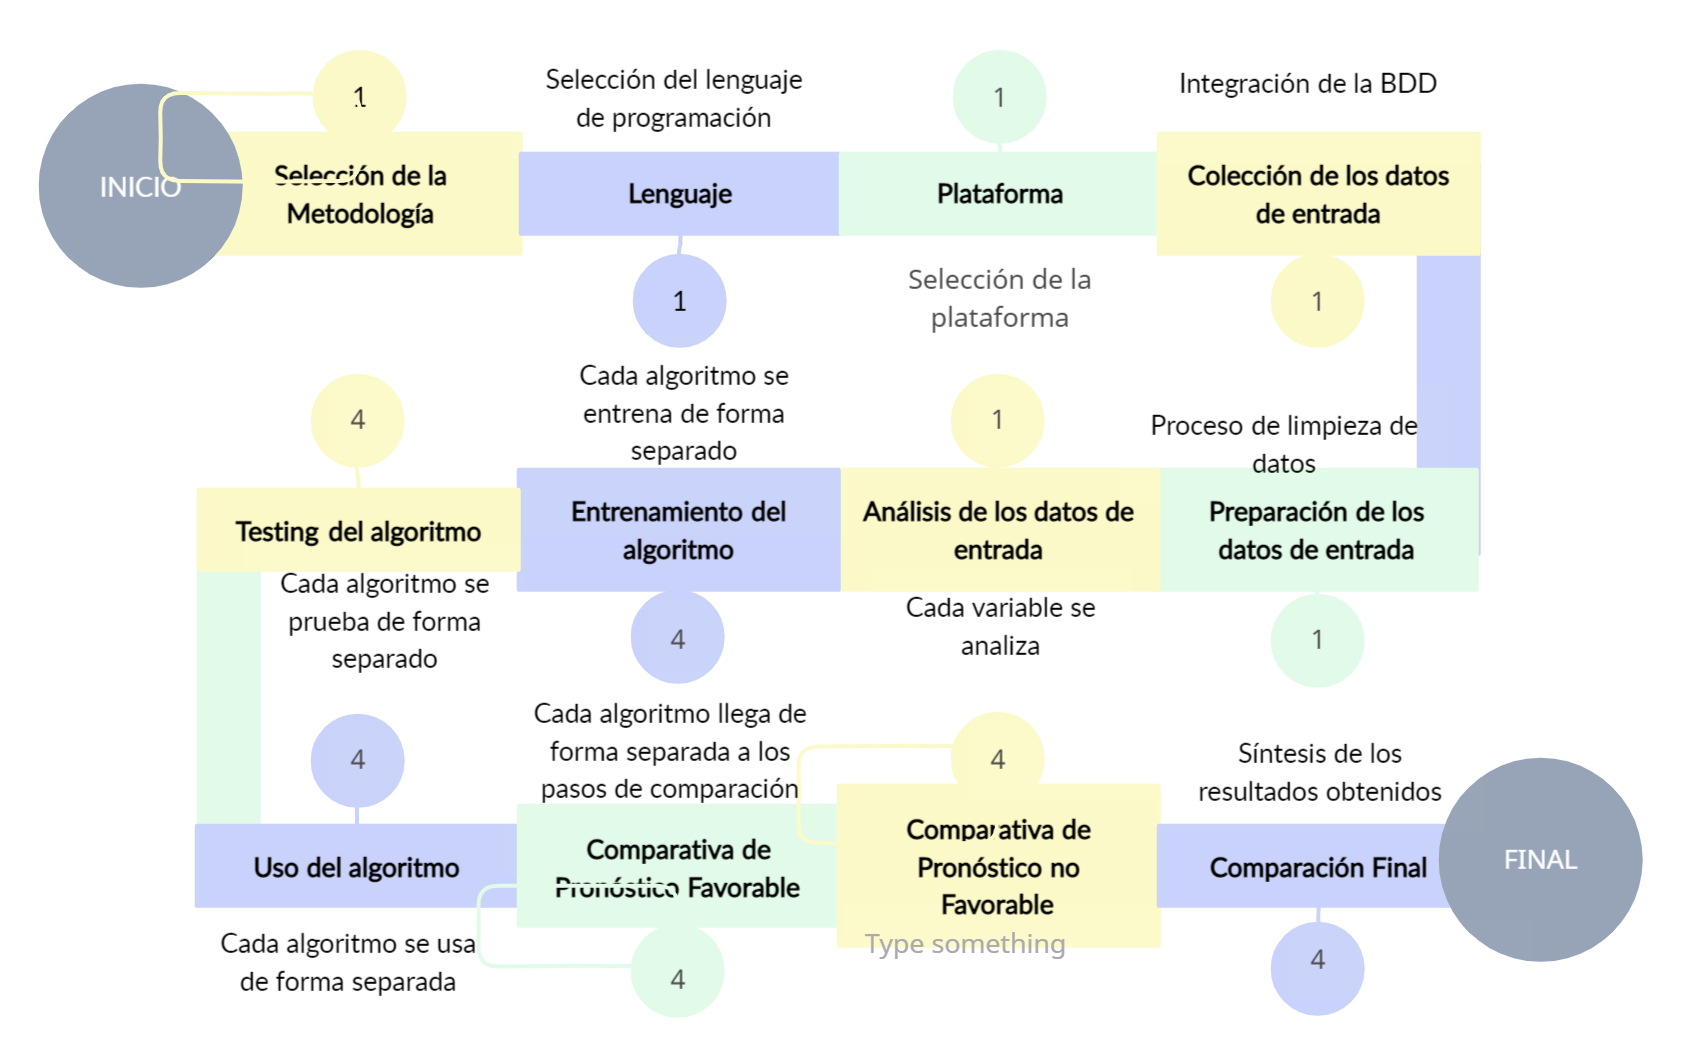
\includegraphics[scale=0.65]{img/mapaDetiempo.png} 
	\caption{Mapa de secuencia metodológica}
	\label{fig:mapaDeTiempo}
\end{figure}


\doublespacing
\subsection{Lenguaje de programación y plataforma}
\spacing{1.5}
Los lenguajes de programación más usados para el ML son Java, R o Python. Para este proyecto se escogió Python por cuatro motivos: 

\begin{enumerate}
	\item Librerías potentes: Python tiene una amplia gama de librerías y frameworks específicos para IA, como TensorFlow, PyTorch, scikit-learn, entre otros, que facilitan la creación y entrenamiento de modelos de IA.
	\item Fácil de aprender: La sintaxis clara y legible de Python hace que sea fácil de aprender y usar para los desarrolladores, lo que significa que se pueden desarrollar modelos de IA de manera más eficiente.
	\item Comunidad activa: La comunidad de Python es activa y colaborativa, lo que significa que hay una gran cantidad de recursos y soluciones disponibles en línea para ayudar a los desarrolladores a resolver cualquier problema que puedan tener.
	\item Interoperabilidad: Python se integra fácilmente con otros lenguajes y tecnologías, lo que significa que se pueden utilizar conjuntamente con otros sistemas y herramientas en proyectos de IA.\\
\end{enumerate}

\par Siguiendo con este razonamiento, para trabajar con el lenguaje Python se puedieron ocupar framework como Tensor Flow, Theano, Amazon Machine Learning, entre otros; al final se optó por la plataforma llamada Jupyter Notebook, popular en la Ciencia de Datos e IA debido a estas ventajas:

\begin{enumerate}
	\item Interfaz interactiva: Jupyter permite a los usuarios ejecutar código en un entorno interactivo y ver los resultados en tiempo real, lo que facilita la exploración y experimentación con datos y modelos de IA.
	\item Documentación integrada: Jupyter permite a los usuarios crear documentos que combinan código, texto, gráficos y otros tipos de contenido multimedia, lo que lo convierte en una excelente opción para la creación de informes y presentaciones de resultados.
	\item Compartir y colaborar: Jupyter permite a los usuarios compartir y colaborar fácilmente en proyectos de IA mediante la creación de notebooks en línea y la posibilidad de trabajar en tiempo real con otros usuarios.
	\item Amplia compatibilidad: Jupyter es compatible con una amplia gama de lenguajes de programación, incluyendo Python, R, Julia, entre otros, lo que significa que los usuarios pueden elegir el lenguaje que mejor se adapte a sus necesidades.\\
\end{enumerate}



     \hypertarget{apliacaciuxf3n-del-muxe9todo}{%
\section{Aplicación}\label{apliacaciuxf3n-del-muxe9todo}}

Para empezar, debemos implementar los pasos sugeridos en la sección 4.2 en el mismo orden que se nos presenta. Los pasos 1, 2 y 3 son comunes para todos los algoritmos, por ende, solo se mostrará una vez en la presente investigación. Al finalizar esta sección se verán los pasos 4, 5 y 6 en cada Algoritmo presentado.

    \hypertarget{colecciuxf3n-de-datos-de-entrada}{%
\section{Colección de datos de
entrada}\label{colecciuxf3n-de-datos-de-entrada}}

El primer paso en el método es la Colección de datos de entrada, en este proceso capturaremos los datos provenientes de la BDD del Hospital Herminda Martín de Chillán y luego diseñaremos un nuevo instrumento.

    \begin{tcolorbox}[breakable, size=fbox, boxrule=1pt, pad at break*=1mm,colback=cellbackground, colframe=cellborder]
\prompt{In}{incolor}{1}{\boxspacing}
\begin{Verbatim}[commandchars=\\\{\}]
\PY{c+c1}{\PYZsh{} Libreria para la manipulación de los datos}
\PY{k+kn}{import} \PY{n+nn}{pandas} \PY{k}{as} \PY{n+nn}{pd}
\PY{k+kn}{import} \PY{n+nn}{numpy} \PY{k}{as} \PY{n+nn}{np}

\PY{c+c1}{\PYZsh{} Leer el dataframe}
\PY{n}{dataframe} \PY{o}{=} \PY{n}{pd}\PY{o}{.}\PY{n}{read\PYZus{}excel}\PY{p}{(}\PY{l+s+s1}{\PYZsq{}}\PY{l+s+s1}{../bdd/bdd\PYZus{}final.xlsx}\PY{l+s+s1}{\PYZsq{}}\PY{p}{)}
\PY{n+nb}{print}\PY{p}{(}\PY{n}{dataframe}\PY{p}{)}
\end{Verbatim}
\end{tcolorbox}

\begin{table}[H]
\centering
\setlength{\tabcolsep}{5pt}
\resizebox{1.0\textwidth}{!}{
	\begin{tabular}{|l|l|l|l|c|l|l|l|l|}
\hline
\multicolumn{1}{|c|}{\textbf{CLAVE}} & \multicolumn{1}{c|}{\textbf{COMUNA}} & \multicolumn{1}{c|}{\textbf{TELEFONOS}} & \multicolumn{1}{c|}{\textbf{EDAD}} & \textbf{...} & \textbf{IL-6   corregida} & \multicolumn{1}{c|}{\textbf{log IL-6}} & \multicolumn{1}{c|}{\textbf{IL-6/VEGF}} & \multicolumn{1}{c|}{\textbf{IL-6/PlGF}} \\ \hline \hline
1 & san carlos &  & 53 & \textbf{...} & 0,156952708 & -0,804 & -0,454839548 & -0,825732298 \\ \hline
2 & coihueco & 41723921-74822219 & 54 & \textbf{...} & 0,012817828 & -1,892 & -0,882899371 & -1,081411325 \\ \hline
3 & chillan & 71818219-50323843 & 78 & \textbf{...} & 0,436365262 & -0,360 & -0,230735564 & -0,296817468 \\ \hline
\multicolumn{1}{|c|}{\textbf{\begin{tabular}[c]{@{}c@{}}.\\ .\\ .\end{tabular}}} & \multicolumn{1}{c|}{\textbf{\begin{tabular}[c]{@{}c@{}}.\\ .\\ .\end{tabular}}} & \multicolumn{1}{c|}{\textbf{\begin{tabular}[c]{@{}c@{}}.\\ .\\ .\end{tabular}}} & \multicolumn{1}{c|}{\textbf{\begin{tabular}[c]{@{}c@{}}.\\ .\\ .\end{tabular}}} & \textbf{...} & \multicolumn{1}{c|}{\textbf{\begin{tabular}[c]{@{}c@{}}.\\ .\\ .\end{tabular}}} & \multicolumn{1}{c|}{\textbf{\begin{tabular}[c]{@{}c@{}}.\\ .\\ .\end{tabular}}} & \multicolumn{1}{c|}{\textbf{\begin{tabular}[c]{@{}c@{}}.\\ .\\ .\end{tabular}}} & \multicolumn{1}{c|}{\textbf{\begin{tabular}[c]{@{}c@{}}.\\ .\\ .\end{tabular}}} \\ \hline
75 & pinto & 82525308 & 79 & \textbf{...} & 0,842328176 & -0,075 & -0,047317636 & -0,08950326 \\ \hline
76 & chillan & 50711724-87107760 & 54 & \textbf{...} & 1,273106319 & 0,105 & 0,054145766 & 0,137865611 \\ \hline
TENS & chillan & 85226191-96473857 & 69 & \textbf{...} & 0,795830574 & -0,099 & \#¡NUM! & \#¡NUM! \\ \hline
\end{tabular}%
}
\caption{Base de datos de pacientes post ACV Isquémico del Hospital Herminda Martin}
\label{tab:bdd}
\end{table}

    \begin{tcolorbox}[breakable, size=fbox, boxrule=1pt, pad at break*=1mm,colback=cellbackground, colframe=cellborder]
\prompt{In}{incolor}{2}{\boxspacing}
\begin{Verbatim}[commandchars=\\\{\}]
\PY{c+c1}{\PYZsh{} Mostramos las variables que posee la base de datos}
\PY{n}{columns\PYZus{}names} \PY{o}{=} \PY{n}{dataframe}\PY{o}{.}\PY{n}{columns}\PY{o}{.}\PY{n}{values}
\PY{n+nb}{print}\PY{p}{(}\PY{n}{columns\PYZus{}names}\PY{p}{)}
\end{Verbatim}
\end{tcolorbox}

    \begin{Verbatim}[commandchars=\\\{\}]
['CLAVE' 'COMUNA' 'TELEFONOS ' 'FICHA CLINICA' 'CTA CTE' 'EDAD' 'PESO'
 'TALLA' 'HTA' 'DIABETES' 'OTRAS PATOLOGIAS' 'FUMA' 'FC' 'PAS' 'PAD'
 'GLUCOSA' 'Hb A/C  \%' 'COL. TOTAL' 'TRIGLICERIDOS' 'LDL' 'HDL' 'HCTO'
 'HB' 'VCM' 'HCM' 'VHS' 'PLAQUETAS' 'INR' 'CONTEO G.B.' 'P.C.R'
 'Nitrogeno Ureico' 'Uremia' 'Creatinina' 'TTPA' 'TP' 'NA' 'K' 'CL'
 'Fosfatasa Alcalina' 'Gamma glutamil' 'Transaminasa piruvica'
 'Trans oxal' 'AREA DE LESION ' 'No  ESTENOSIS INTRACRANEAL'
 'No  ESTENOSIS EXTRACRANEAL' '\%  ESTENOSIS INTRACRANEAL'
 '\%  ESTENOSIS EXTRACRANEAL' 'GLASGOW AL INICO ACV' 'NIHSS INICO ACV'
 'RANKIN INICIO ACV' 'NIHSS alta ACV' 'RANKIN alta ACV' 'NIHSS 6M'
 'RANKIN 6M' 'diag Elopez' 'DIAG. NEUROLOGICO' 'Diag2' 'Diag3'
 'FECHA TOMA MUESTRA' 'Estado paciente' 'Fecha defuncion'
 'CAUSA  DEFUNCION ' 'MOTIVO DE DESCARTE ' 'TROMBOLISIS' 'eduardo'
 'sirve ' 'escala' 'exosomes 1' 'exosomes 2' 'VEGF ab1' 'VEGF ab2'
 'VEGF prome' 'plgf mg prot' 'plgf mg prot.1' 'plgf promedio' 'logVEGF'
 'logPlGF' 'logPCR' 'PCR/VEGF ratio' 'PCR/PLGF ratio' 'IL-6 (pg/ml)'
 'IL-6 corregida' 'log IL-6' 'IL-6/VEGF' 'IL-6/PlGF']
    \end{Verbatim}

    Mostramos la cantidad de pacientes y variables(columnas) que posee la
BDD:

    \begin{tcolorbox}[breakable, size=fbox, boxrule=1pt, pad at break*=1mm,colback=cellbackground, colframe=cellborder]
\prompt{In}{incolor}{3}{\boxspacing}
\begin{Verbatim}[commandchars=\\\{\}]
\PY{n+nb}{print}\PY{p}{(}\PY{l+s+s1}{\PYZsq{}}\PY{l+s+s1}{Existen }\PY{l+s+si}{\PYZob{}\PYZcb{}}\PY{l+s+s1}{ pacientes con }\PY{l+s+si}{\PYZob{}\PYZcb{}}\PY{l+s+s1}{ variables.}\PY{l+s+s1}{\PYZsq{}}\PY{o}{.}\PY{n}{format}\PY{p}{(}\PY{o}{*}\PY{n}{dataframe}\PY{o}{.}\PY{n}{shape}\PY{p}{)}\PY{p}{)}
\PY{n+nb}{print}\PY{p}{(}\PY{l+s+s2}{\PYZdq{}}\PY{l+s+s2}{Existen}\PY{l+s+s2}{\PYZdq{}}\PY{p}{,} \PY{n}{dataframe}\PY{o}{.}\PY{n}{size}\PY{p}{,} \PY{l+s+s2}{\PYZdq{}}\PY{l+s+s2}{elementos}\PY{l+s+s2}{\PYZdq{}}\PY{p}{)}
\end{Verbatim}
\end{tcolorbox}

    \begin{Verbatim}[commandchars=\\\{\}]
Existen 75 pacientes con 85 variables.
Existen 6375 elementos
    \end{Verbatim}

    Se observa que la BDD posee muchas variables y pocos pacientes registrados en las tuplas. Esto hará que sea más difícil la predicción para los algoritmos, así que necesitamos un nuevo instrumento.

    \hypertarget{diseuxf1o-del-instrumento}{%
\subsection{Diseño del instrumento}\label{diseuxf1o-del-instrumento}}

Desde el punto de vista científico, para que un estudio salga lo más certero posible necesitamos variables significativas para la investigación y con la menor pérdida de datos posible. En la BDD todas las variables presentan importancia, algunas son imprescindibles para la investigación, otras con pocos datos completados o simplemente las variables sujetas a interpretación médica (humana). Debido a lo anterior se seleccionaron las variables por dos motivos, el primero fue porque eran las que estaban más completas en la BDD y el segundo porque se determinó que eran más significativas para la investigación por estudios realizados al ACV y dataset presentes en internet. A continuación, se mostrarán las variables escogidas y una pequeña descripción de ellas.

    \begin{quote}
\textbf{HTA}: \texttt{"si"\ o\ "no",\ HIPERTENSIÓN}
\end{quote}

\begin{quote}
\textbf{DIABETES}: \texttt{"si"\ o\ "no"}
\end{quote}

\begin{quote}
\textbf{EDAD}: \texttt{Edad\ del\ paciente}
\end{quote}

\begin{quote}
\textbf{GLUCOSA}: \texttt{Nivel\ de\ azúcar\ en\ la\ sangre}
\end{quote}

\begin{quote}
\textbf{COL. TOTAL}: \texttt{Cantidad\ de\ Colesterol\ en\ la\ sangre}
\end{quote}

\begin{quote}
\textbf{TRIGLICERIDOS}:
\texttt{Cantidad\ de\ triglicéridos\ en\ la\ sangre}
\end{quote}

\begin{quote}
\textbf{INR}:
\texttt{Índice\ internacional\ normalizado\ (INR,\ por\ sus\ siglas\ en\ inglés)\ es\ un\ tipo\ de\ cálculo\ que\ se\ basa\ en\ los\ resultados\ de\ las\ pruebas\ de\ tiempo\ de\ protrombina}
\end{quote}

\begin{quote}
\textbf{CONTEO G.B.}:
\texttt{Conteo\ de\ glóbulos\ blancos\ en\ la\ sangre}
\end{quote}

\begin{quote}
\textbf{GLASGOW AL INICO ACV}:
\texttt{Escala\ de\ 15\ puntos\ médica\ que\ es\ para\ medir\ el\ estado\ de\ conciencia.\ Esta\ pertence\ a\ la\ Inicial}
\end{quote}

\begin{quote}
\textbf{NIHSS INICO ACV}:
\texttt{Escala\ de\ 42\ puntos\ más\ empleada\ para\ la\ valoración\ de\ funciones\ neurológicas\ básicas\ en\ la\ fase\ aguda\ del\ ictus\ isquémico,\ tanto\ al\ inicio\ como\ durante\ su\ evolución.\ Esta\ pertence\ a\ la\ Inicial}
\end{quote}

\begin{quote}
\textbf{NIHSS alta ACV}:
\texttt{Pertenece\ cuando\ es\ dado\ de\ alta\ el\ paciente}
\end{quote}

    La Hipertensión Arterial y la Diabetes son factores de riesgo altos en cualquier enfermedad no trasmisible, por esto son de las primeras seleccionadas, que además contaremos con las escalas de Glasgow y NIHSS que son escalas internacionales para la evaluación del ACV Isquémico.

    \hypertarget{preparaciuxf3n-de-los-datos-de-entrada}{%
\section{Preparación de los datos de
entrada}\label{preparaciuxf3n-de-los-datos-de-entrada}}

El segundo paso descrito en la metodología  es un paso crítico y uno de los más extensos en el desarrollo de proyectos de ML. Aqui se llevará a cabo una limpieza de datos, como la eliminicaión de registros o rescatar datos nulos; selección de caracteristicas que sean relevantes para la investigación; transformación de caracteristicas, que serán para escalar datos para que se adecuen al modelo de ML.

    \hypertarget{eliminaciuxf3n-las-filas-de-los-pacientes-que-se-expulsaron-de-la-bdd}{%
\subsection{Eliminación valores nulos}\label{eliminaciuxf3n-las-filas-de-los-pacientes-que-se-expulsaron-de-la-bdd}}

Como se indicó anteriormente, se dispone de 75 tuplas con 85 columnas, con un total de 6375 elementos, que se planean disminuir por indicación del médico que facilitó la base de datos. La indicación fue que había pacientes que fueron retirados del programa y estaban marcados con un ``out'' en la variable de ``diag Elopez''.

    \begin{tcolorbox}[breakable, size=fbox, boxrule=1pt, pad at break*=1mm,colback=cellbackground, colframe=cellborder]
\prompt{In}{incolor}{4}{\boxspacing}
\begin{Verbatim}[commandchars=\\\{\}]
\PY{n}{dataframe}\PY{o}{.}\PY{n}{drop}\PY{p}{(}\PY{n}{dataframe}\PY{p}{[}\PY{p}{(}\PY{n}{dataframe}\PY{p}{[}\PY{l+s+s1}{\PYZsq{}}\PY{l+s+s1}{diag Elopez}\PY{l+s+s1}{\PYZsq{}}\PY{p}{]} \PY{o}{==} \PY{l+s+s1}{\PYZsq{}}\PY{l+s+s1}{out}\PY{l+s+s1}{\PYZsq{}}\PY{p}{)}\PY{p}{]}\PY{o}{.}\PY{n}{index}\PY{p}{,} \PY{n}{inplace}\PY{o}{=}\PY{k+kc}{True}\PY{p}{)}

\PY{c+c1}{\PYZsh{} mostramos 10 columnas}
\PY{n}{pd}\PY{o}{.}\PY{n}{options}\PY{o}{.}\PY{n}{display}\PY{o}{.}\PY{n}{max\PYZus{}columns} \PY{o}{=} \PY{l+m+mi}{10}

\PY{c+c1}{\PYZsh{} Mostramos las primeras 7 tuplas}
\PY{n}{dataframe}\PY{o}{.}\PY{n}{head}\PY{p}{(}\PY{l+m+mi}{7}\PY{p}{)}
\end{Verbatim}
\end{tcolorbox}

\begin{table}[H]
\centering
\setlength{\tabcolsep}{5pt}
\resizebox{1.0\textwidth}{!}{
	\begin{tabular}{|l|l|l|l|c|l|l|l|l|}
\hline
\multicolumn{1}{|c|}{\textbf{CLAVE}} & \multicolumn{1}{c|}{\textbf{COMUNA}} & \multicolumn{1}{c|}{\textbf{TELEFONOS}} & \multicolumn{1}{c|}{\textbf{EDAD}} & \textbf{...} & \textbf{IL-6   corregida} & \multicolumn{1}{c|}{\textbf{log IL-6}} & \multicolumn{1}{c|}{\textbf{IL-6/VEGF}} & \multicolumn{1}{c|}{\textbf{IL-6/PlGF}} \\ \hline \hline
1 & san carlos &  & 53 & \textbf{...} & 0,156952708 & -0,804 & -0,454839548 & -0,825732298 \\ \hline
2 & coihueco & 41723921-74822219 & 54 & \textbf{...} & 0,012817828 & -1,892 & -0,882899371 & -1,081411325 \\ \hline
3 & chillan & 71818219-50323843 & 78 & \textbf{...} & 0,436365262 & -0,360 & -0,230735564 & -0,296817468 \\ \hline
\multicolumn{1}{|c|}{\textbf{\begin{tabular}[c]{@{}c@{}}.\\ .\\ .\end{tabular}}} & \multicolumn{1}{c|}{\textbf{\begin{tabular}[c]{@{}c@{}}.\\ .\\ .\end{tabular}}} & \multicolumn{1}{c|}{\textbf{\begin{tabular}[c]{@{}c@{}}.\\ .\\ .\end{tabular}}} & \multicolumn{1}{c|}{\textbf{\begin{tabular}[c]{@{}c@{}}.\\ .\\ .\end{tabular}}} & \textbf{...} & \multicolumn{1}{c|}{\textbf{\begin{tabular}[c]{@{}c@{}}.\\ .\\ .\end{tabular}}} & \multicolumn{1}{c|}{\textbf{\begin{tabular}[c]{@{}c@{}}.\\ .\\ .\end{tabular}}} & \multicolumn{1}{c|}{\textbf{\begin{tabular}[c]{@{}c@{}}.\\ .\\ .\end{tabular}}} & \multicolumn{1}{c|}{\textbf{\begin{tabular}[c]{@{}c@{}}.\\ .\\ .\end{tabular}}} \\ \hline
75 & pinto & 82525308 & 79 & \textbf{...} & 0,842328176 & -0,075 & -0,047317636 & -0,08950326 \\ \hline
76 & chillan & 50711724-87107760 & 54 & \textbf{...} & 1,273106319 & 0,105 & 0,054145766 & 0,137865611 \\ \hline
TENS & chillan & 85226191-96473857 & 69 & \textbf{...} & 0,795830574 & -0,099 & \#¡NUM! & \#¡NUM! \\ \hline
\end{tabular}%
}
\caption{Eliminación de pacientes que no aportan en la investigación}
\label{tab:bdd}
\end{table}
        
    \begin{tcolorbox}[breakable, size=fbox, boxrule=1pt, pad at break*=1mm,colback=cellbackground, colframe=cellborder]
\prompt{In}{incolor}{5}{\boxspacing}
\begin{Verbatim}[commandchars=\\\{\}]
\PY{n+nb}{print}\PY{p}{(}\PY{l+s+s1}{\PYZsq{}}\PY{l+s+s1}{Existen }\PY{l+s+si}{\PYZob{}\PYZcb{}}\PY{l+s+s1}{ pacientes con }\PY{l+s+si}{\PYZob{}\PYZcb{}}\PY{l+s+s1}{ variables.}\PY{l+s+s1}{\PYZsq{}}\PY{o}{.}\PY{n}{format}\PY{p}{(}\PY{o}{*}\PY{n}{dataframe}\PY{o}{.}\PY{n}{shape}\PY{p}{)}\PY{p}{)}
\PY{n+nb}{print}\PY{p}{(}\PY{l+s+s2}{\PYZdq{}}\PY{l+s+s2}{Existen}\PY{l+s+s2}{\PYZdq{}}\PY{p}{,} \PY{n}{dataframe}\PY{o}{.}\PY{n}{size}\PY{p}{,} \PY{l+s+s2}{\PYZdq{}}\PY{l+s+s2}{elementos}\PY{l+s+s2}{\PYZdq{}}\PY{p}{)}
\end{Verbatim}
\end{tcolorbox}

    \begin{Verbatim}[commandchars=\\\{\}]
Existen 46 pacientes con 85 variables.
Existen 3910 elementos
    \end{Verbatim}

    \hypertarget{variables-significativas-para-la-investigaciuxf3n}{%
\subsection{Variables significativas para la
investigación}\label{variables-significativas-para-la-investigaciuxf3n}}

Ahora asignamos las variables significativas, para esto se extrae la información del marco de trabajo, identificando las variables categóricas para un arreglo completamente nuevo y así empezar a trabajar sobre el nuevo archivo.

    \begin{tcolorbox}[breakable, size=fbox, boxrule=1pt, pad at break*=1mm,colback=cellbackground, colframe=cellborder]
\prompt{In}{incolor}{6}{\boxspacing}
\begin{Verbatim}[commandchars=\\\{\}]
\PY{c+c1}{\PYZsh{} Tomaremos las variables más significativas para la investigación}
\PY{n}{columnasMuestra} \PY{o}{=} \PY{p}{[}\PY{l+s+s1}{\PYZsq{}}\PY{l+s+s1}{HTA}\PY{l+s+s1}{\PYZsq{}}\PY{p}{,} \PY{l+s+s1}{\PYZsq{}}\PY{l+s+s1}{DIABETES}\PY{l+s+s1}{\PYZsq{}}\PY{p}{,} \PY{l+s+s1}{\PYZsq{}}\PY{l+s+s1}{EDAD}\PY{l+s+s1}{\PYZsq{}}\PY{p}{,} \PY{l+s+s1}{\PYZsq{}}\PY{l+s+s1}{GLUCOSA}\PY{l+s+s1}{\PYZsq{}}\PY{p}{,} \PY{l+s+s1}{\PYZsq{}}\PY{l+s+s1}{COL. TOTAL}\PY{l+s+s1}{\PYZsq{}}\PY{p}{,} \PY{l+s+s1}{\PYZsq{}}\PY{l+s+s1}{TRIGLICERIDOS}\PY{l+s+s1}{\PYZsq{}}\PY{p}{,} \PY{l+s+s1}{\PYZsq{}}\PY{l+s+s1}{INR}\PY{l+s+s1}{\PYZsq{}}\PY{p}{,} \PY{l+s+s1}{\PYZsq{}}\PY{l+s+s1}{CONTEO G.B.}\PY{l+s+s1}{\PYZsq{}}\PY{p}{,} \PY{l+s+s1}{\PYZsq{}}\PY{l+s+s1}{GLASGOW AL INICO ACV}\PY{l+s+s1}{\PYZsq{}}\PY{p}{,} \PY{l+s+s1}{\PYZsq{}}\PY{l+s+s1}{NIHSS INICO ACV}\PY{l+s+s1}{\PYZsq{}}\PY{p}{,} \PY{l+s+s1}{\PYZsq{}}\PY{l+s+s1}{NIHSS alta ACV}\PY{l+s+s1}{\PYZsq{}}\PY{p}{]}
\PY{n}{dataset} \PY{o}{=} \PY{n}{dataframe}\PY{p}{[}\PY{p}{[}\PY{o}{*}\PY{n}{columnasMuestra}\PY{p}{]}\PY{p}{]}

\PY{c+c1}{\PYZsh{} Muestramos las columnas que se ajusten a la cantidad de espacio}
\PY{n}{pd}\PY{o}{.}\PY{n}{options}\PY{o}{.}\PY{n}{display}\PY{o}{.}\PY{n}{max\PYZus{}columns} \PY{o}{=} \PY{l+m+mi}{0}

\PY{n}{dataset}\PY{o}{.}\PY{n}{head}\PY{p}{(}\PY{l+m+mi}{5}\PY{p}{)}
\end{Verbatim}
\end{tcolorbox}

\begin{table}[H]
\centering
\setlength{\tabcolsep}{5pt}
\resizebox{1.0\textwidth}{!}{
\begin{tabular}{|l|l|l|l|l|l|l|l|l|l|l|}
\hline
\multicolumn{1}{|c|}{\textbf{HTA}} & \multicolumn{1}{c|}{\textbf{DIABETES}} & \multicolumn{1}{c|}{\textbf{EDAD}} & \multicolumn{1}{c|}{\textbf{GLUCOSA}} & \multicolumn{1}{c|}{\textbf{COL. TOTAL}} & \multicolumn{1}{c|}{\textbf{TRIGLICERIDOS}} & \multicolumn{1}{c|}{\textbf{INR}} & \multicolumn{1}{c|}{\textbf{CONTEO G.B.}} & \multicolumn{1}{c|}{\textbf{GLASGOW AL INICO   ACV}} & \multicolumn{1}{c|}{\textbf{NIHSS INICO ACV}} & \multicolumn{1}{c|}{\textbf{NIHSS alta ACV}} \\ \hline \hline
 &  & 53 & 137,09 & 268 & 130 & 1,08 & 41,9 & 11 & 14 & 42 \\ \hline
si & si & 54 &  & 187 & 130 &  & 8,3 & 15 & 6 & 0 \\ \hline
si & si & 78 & 359,42 & 159 & 97 & 0,89 & 8,5 & 15 & 5 & 2 \\ \hline
\multicolumn{1}{|c|}{\textbf{\begin{tabular}[c]{@{}c@{}}.\\ .\\ .\end{tabular}}} & \multicolumn{1}{c|}{\textbf{\begin{tabular}[c]{@{}c@{}}.\\ .\\ .\end{tabular}}} & \multicolumn{1}{c|}{\textbf{\begin{tabular}[c]{@{}c@{}}.\\ .\\ .\end{tabular}}} & \multicolumn{1}{c|}{\textbf{\begin{tabular}[c]{@{}c@{}}.\\ .\\ .\end{tabular}}} & \multicolumn{1}{c|}{\textbf{\begin{tabular}[c]{@{}c@{}}.\\ .\\ .\end{tabular}}} & \multicolumn{1}{c|}{\textbf{\begin{tabular}[c]{@{}c@{}}.\\ .\\ .\end{tabular}}} & \multicolumn{1}{c|}{\textbf{\begin{tabular}[c]{@{}c@{}}.\\ .\\ .\end{tabular}}} & \multicolumn{1}{c|}{\textbf{\begin{tabular}[c]{@{}c@{}}.\\ .\\ .\end{tabular}}} & \multicolumn{1}{c|}{\textbf{\begin{tabular}[c]{@{}c@{}}.\\ .\\ .\end{tabular}}} & \multicolumn{1}{c|}{\textbf{\begin{tabular}[c]{@{}c@{}}.\\ .\\ .\end{tabular}}} & \multicolumn{1}{c|}{\textbf{\begin{tabular}[c]{@{}c@{}}.\\ .\\ .\end{tabular}}} \\ \hline
si & si & 79 & 116,99 & 109 & 118 &  & 9,9 &  & 2 & 2 \\ \hline
si & si & 54 & 211,58 &  &  & 0,99 & 6,5 & 15 & 1 & 1 \\ \hline
si & si & 69 & 217,21 & 202 & 232 & 1,03 & 10,4 & 0 &  &  \\ \hline
\end{tabular}%
}
\caption{Dataset de variables para la investigación}
\label{tab:dataset}
\end{table}
        
    Mostramos la cantidad de pacientes y variables/columnas que posee la BDD después de la selección de variables significativas para la investigación:

    \begin{tcolorbox}[breakable, size=fbox, boxrule=1pt, pad at break*=1mm,colback=cellbackground, colframe=cellborder]
\prompt{In}{incolor}{7}{\boxspacing}
\begin{Verbatim}[commandchars=\\\{\}]
\PY{n+nb}{print}\PY{p}{(}\PY{l+s+s1}{\PYZsq{}}\PY{l+s+s1}{Existen }\PY{l+s+si}{\PYZob{}\PYZcb{}}\PY{l+s+s1}{ pacientes con }\PY{l+s+si}{\PYZob{}\PYZcb{}}\PY{l+s+s1}{ variables.}\PY{l+s+s1}{\PYZsq{}}\PY{o}{.}\PY{n}{format}\PY{p}{(}\PY{o}{*}\PY{n}{dataset}\PY{o}{.}\PY{n}{shape}\PY{p}{)}\PY{p}{)}
\PY{n+nb}{print}\PY{p}{(}\PY{l+s+s2}{\PYZdq{}}\PY{l+s+s2}{Existen}\PY{l+s+s2}{\PYZdq{}}\PY{p}{,} \PY{n}{dataset}\PY{o}{.}\PY{n}{size}\PY{p}{,} \PY{l+s+s2}{\PYZdq{}}\PY{l+s+s2}{elementos}\PY{l+s+s2}{\PYZdq{}}\PY{p}{)}
\end{Verbatim}
\end{tcolorbox}

    \begin{Verbatim}[commandchars=\\\{\}]
Existen 46 pacientes con 11 variables.
Existen 506 elementos
    \end{Verbatim}

    \hypertarget{descripciuxf3n-general-de-los-datos}{%
\subsection{Descripción general de los
datos}\label{descripciuxf3n-general-de-los-datos}}

En la descripción de los datos, se muestran parámetros, pérdida de datos (Missing Data), forma y su descripción estadística.

    \begin{tcolorbox}[breakable, size=fbox, boxrule=1pt, pad at break*=1mm,colback=cellbackground, colframe=cellborder]
\prompt{In}{incolor}{8}{\boxspacing}
\begin{Verbatim}[commandchars=\\\{\}]
\PY{c+c1}{\PYZsh{} Check Dataset:}
\PY{k}{def} \PY{n+nf}{check\PYZus{}data}\PY{p}{(}\PY{n}{dataset}\PY{p}{,}\PY{n}{head}\PY{o}{=}\PY{l+m+mi}{5}\PY{p}{)}\PY{p}{:}
    \PY{n+nb}{print}\PY{p}{(}\PY{l+m+mi}{20}\PY{o}{*}\PY{l+s+s2}{\PYZdq{}}\PY{l+s+s2}{\PYZhy{}}\PY{l+s+s2}{\PYZdq{}} \PY{o}{+} \PY{l+s+s2}{\PYZdq{}}\PY{l+s+s2}{Información}\PY{l+s+s2}{\PYZdq{}}\PY{o}{.}\PY{n}{center}\PY{p}{(}\PY{l+m+mi}{20}\PY{p}{)} \PY{o}{+} \PY{l+m+mi}{20}\PY{o}{*}\PY{l+s+s2}{\PYZdq{}}\PY{l+s+s2}{\PYZhy{}}\PY{l+s+s2}{\PYZdq{}}\PY{p}{)}
    \PY{n+nb}{print}\PY{p}{(}\PY{n}{dataset}\PY{o}{.}\PY{n}{info}\PY{p}{(}\PY{p}{)}\PY{p}{)}
    \PY{n+nb}{print}\PY{p}{(}\PY{l+m+mi}{20}\PY{o}{*}\PY{l+s+s2}{\PYZdq{}}\PY{l+s+s2}{\PYZhy{}}\PY{l+s+s2}{\PYZdq{}} \PY{o}{+} \PY{l+s+s2}{\PYZdq{}}\PY{l+s+s2}{Forma de datos}\PY{l+s+s2}{\PYZdq{}}\PY{o}{.}\PY{n}{center}\PY{p}{(}\PY{l+m+mi}{20}\PY{p}{)} \PY{o}{+} \PY{l+m+mi}{20}\PY{o}{*}\PY{l+s+s2}{\PYZdq{}}\PY{l+s+s2}{\PYZhy{}}\PY{l+s+s2}{\PYZdq{}}\PY{p}{)}
    \PY{n+nb}{print}\PY{p}{(}\PY{n}{dataset}\PY{o}{.}\PY{n}{shape}\PY{p}{)}
    \PY{n+nb}{print}\PY{p}{(}\PY{l+s+s2}{\PYZdq{}}\PY{l+s+se}{\PYZbs{}n}\PY{l+s+s2}{\PYZdq{}} \PY{o}{+} \PY{l+m+mi}{20}\PY{o}{*}\PY{l+s+s2}{\PYZdq{}}\PY{l+s+s2}{\PYZhy{}}\PY{l+s+s2}{\PYZdq{}} \PY{o}{+} \PY{l+s+s2}{\PYZdq{}}\PY{l+s+s2}{Los primeros 5 datos}\PY{l+s+s2}{\PYZdq{}}\PY{o}{.}\PY{n}{center}\PY{p}{(}\PY{l+m+mi}{20}\PY{p}{)} \PY{o}{+} \PY{l+m+mi}{20}\PY{o}{*}\PY{l+s+s2}{\PYZdq{}}\PY{l+s+s2}{\PYZhy{}}\PY{l+s+s2}{\PYZdq{}}\PY{p}{)}
    \PY{n+nb}{print}\PY{p}{(}\PY{n}{dataset}\PY{o}{.}\PY{n}{head}\PY{p}{(}\PY{p}{)}\PY{p}{)}
    \PY{n+nb}{print}\PY{p}{(}\PY{l+s+s2}{\PYZdq{}}\PY{l+s+se}{\PYZbs{}n}\PY{l+s+s2}{\PYZdq{}} \PY{o}{+} \PY{l+m+mi}{20} \PY{o}{*} \PY{l+s+s2}{\PYZdq{}}\PY{l+s+s2}{\PYZhy{}}\PY{l+s+s2}{\PYZdq{}} \PY{o}{+} \PY{l+s+s2}{\PYZdq{}}\PY{l+s+s2}{Los últimos 5 datos}\PY{l+s+s2}{\PYZdq{}}\PY{o}{.}\PY{n}{center}\PY{p}{(}\PY{l+m+mi}{20}\PY{p}{)} \PY{o}{+} \PY{l+m+mi}{20} \PY{o}{*} \PY{l+s+s2}{\PYZdq{}}\PY{l+s+s2}{\PYZhy{}}\PY{l+s+s2}{\PYZdq{}}\PY{p}{)}
    \PY{n+nb}{print}\PY{p}{(}\PY{n}{dataset}\PY{o}{.}\PY{n}{tail}\PY{p}{(}\PY{p}{)}\PY{p}{)}
    \PY{n+nb}{print}\PY{p}{(}\PY{l+s+s2}{\PYZdq{}}\PY{l+s+se}{\PYZbs{}n}\PY{l+s+s2}{\PYZdq{}} \PY{o}{+} \PY{l+m+mi}{20} \PY{o}{*} \PY{l+s+s2}{\PYZdq{}}\PY{l+s+s2}{\PYZhy{}}\PY{l+s+s2}{\PYZdq{}} \PY{o}{+} \PY{l+s+s2}{\PYZdq{}}\PY{l+s+s2}{Missing Data}\PY{l+s+s2}{\PYZdq{}}\PY{o}{.}\PY{n}{center}\PY{p}{(}\PY{l+m+mi}{20}\PY{p}{)} \PY{o}{+} \PY{l+m+mi}{20} \PY{o}{*} \PY{l+s+s2}{\PYZdq{}}\PY{l+s+s2}{\PYZhy{}}\PY{l+s+s2}{\PYZdq{}}\PY{p}{)}
    \PY{n+nb}{print}\PY{p}{(}\PY{n}{dataset}\PY{o}{.}\PY{n}{isnull}\PY{p}{(}\PY{p}{)}\PY{o}{.}\PY{n}{sum}\PY{p}{(}\PY{p}{)}\PY{p}{)}
    \PY{n+nb}{print}\PY{p}{(}\PY{l+s+s2}{\PYZdq{}}\PY{l+s+se}{\PYZbs{}n}\PY{l+s+s2}{\PYZdq{}} \PY{o}{+} \PY{l+m+mi}{20} \PY{o}{*} \PY{l+s+s2}{\PYZdq{}}\PY{l+s+s2}{\PYZhy{}}\PY{l+s+s2}{\PYZdq{}} \PY{o}{+} \PY{l+s+s2}{\PYZdq{}}\PY{l+s+s2}{Describir los datos}\PY{l+s+s2}{\PYZdq{}}\PY{o}{.}\PY{n}{center}\PY{p}{(}\PY{l+m+mi}{20}\PY{p}{)} \PY{o}{+} \PY{l+m+mi}{20} \PY{o}{*} \PY{l+s+s2}{\PYZdq{}}\PY{l+s+s2}{\PYZhy{}}\PY{l+s+s2}{\PYZdq{}}\PY{p}{)}
    \PY{n+nb}{print}\PY{p}{(}\PY{n}{dataset}\PY{o}{.}\PY{n}{describe}\PY{p}{(}\PY{p}{)}\PY{o}{.}\PY{n}{T}\PY{p}{)}
\PY{n}{check\PYZus{}data}\PY{p}{(}\PY{n}{dataset}\PY{p}{)}
\end{Verbatim}
\end{tcolorbox}

    \begin{Verbatim}[commandchars=\\\{\}]
--------------------    Información     --------------------
<class 'pandas.core.frame.DataFrame'>
Int64Index: 46 entries, 0 to 74
Data columns (total 11 columns):
 \#   Column                Non-Null Count  Dtype
---  ------                --------------  -----
 0   HTA                   42 non-null     object
 1   DIABETES              34 non-null     object
 2   EDAD                  44 non-null     float64
 3   GLUCOSA               38 non-null     float64
 4   COL. TOTAL            40 non-null     float64
 5   TRIGLICERIDOS         40 non-null     float64
 6   INR                   37 non-null     float64
 7   CONTEO G.B.           46 non-null     float64
 8   GLASGOW AL INICO ACV  29 non-null     float64
 9   NIHSS INICO ACV       39 non-null     float64
 10  NIHSS alta ACV        32 non-null     float64
dtypes: float64(9), object(2)
memory usage: 4.3+ KB
None
--------------------   Forma de datos   --------------------
(46, 11)

--------------------Los primeros 5 datos--------------------
   HTA DIABETES  {\ldots}  NIHSS INICO ACV  NIHSS alta ACV
0  NaN      NaN  {\ldots}             14.0            42.0
1   si       si  {\ldots}              6.0             0.0
2   si       si  {\ldots}              5.0             2.0
3   si       si  {\ldots}              1.0             0.0
4   si       si  {\ldots}              3.0             2.0

[5 rows x 11 columns]

--------------------Los últimos 5 datos --------------------
   HTA DIABETES  {\ldots}  NIHSS INICO ACV  NIHSS alta ACV
68  si       no  {\ldots}              NaN             NaN
69  no       no  {\ldots}              2.0             0.0
72  si       si  {\ldots}              2.0             2.0
73  si       si  {\ldots}              1.0             1.0
74  si       si  {\ldots}              NaN             NaN

[5 rows x 11 columns]

--------------------    Missing Data    --------------------
HTA                      4
DIABETES                12
EDAD                     2
GLUCOSA                  8
COL. TOTAL               6
TRIGLICERIDOS            6
INR                      9
CONTEO G.B.              0
GLASGOW AL INICO ACV    17
NIHSS INICO ACV          7
NIHSS alta ACV          14
dtype: int64

--------------------Describir los datos --------------------
                      count        mean  {\ldots}       75\%     max
EDAD                   44.0   71.522727  {\ldots}   80.5000   90.00
GLUCOSA                38.0  135.529211  {\ldots}  162.5925  359.42
COL. TOTAL             40.0  162.750000  {\ldots}  188.5000  342.00
TRIGLICERIDOS          40.0  123.450000  {\ldots}  142.0000  232.00
INR                    37.0    1.197568  {\ldots}    1.2000    3.08
CONTEO G.B.            46.0   10.119783  {\ldots}   10.3750   41.90
GLASGOW AL INICO ACV   29.0   13.482759  {\ldots}   15.0000   15.00
NIHSS INICO ACV        39.0    5.564103  {\ldots}    6.5000   21.00
NIHSS alta ACV         32.0    5.687500  {\ldots}    4.0000   42.00

[9 rows x 8 columns]
    \end{Verbatim}

    La descripción de los datos nos ayuda a evaluar los casos particulares de las variables que serán tratadas en los siguientes títulos.

    \hypertarget{missing-data}{%
\subsection{Missing data}\label{missing-data}}

Los datos que faltan ocurren cuando no se almacena ningún valor en la variable de observación. Aunque el Missing data es una ocurrencia muy común, estos pueden tener una presión significativa en los resultados de la aplicación del instrumento. Para corregir este problema, existen variadas técnicas estadísticas, siendo una de ellas la mediana y el redondeo como lo muestra \cite{Bar2017} en algunas variables que utilizaremos para llenar las celdas faltantes. Tomaremos la información que mostramos anteriormente.

    \begin{tcolorbox}[breakable, size=fbox, boxrule=1pt, pad at break*=1mm,colback=cellbackground, colframe=cellborder]
\prompt{In}{incolor}{9}{\boxspacing}
\begin{Verbatim}[commandchars=\\\{\}]
\PY{n}{dataset}\PY{o}{.}\PY{n}{isnull}\PY{p}{(}\PY{p}{)}\PY{o}{.}\PY{n}{sum}\PY{p}{(}\PY{p}{)}
\end{Verbatim}
\end{tcolorbox}

\begin{table}[H]
\centering
\setlength{\tabcolsep}{5pt}
\resizebox{0.5\textwidth}{!}{
	\begin{tabular}{|r|r|}
\hline
\multicolumn{1}{|l|}{\textbf{}} & \multicolumn{1}{c|}{\textbf{MISSING DATA}} \\ \hline \hline
\textbf{HTA } & 4 \\ \hline
\textbf{DIABETES } & 12 \\ \hline
\textbf{EDAD } & 2 \\ \hline
\textbf{GLUCOSA } & 8 \\ \hline
\textbf{COL. TOTAL } & 6 \\ \hline
\textbf{TRIGLICERIDOS } & 6 \\ \hline
\textbf{INR } & 9 \\ \hline
\textbf{CONTEO G.B. } & 0 \\ \hline
\textbf{ GLASGOW AL INICO ACV } & 17 \\ \hline
\textbf{NIHSS INICO ACV } & 7 \\ \hline
\textbf{NIHSS alta ACV } & 14 \\ \hline
\end{tabular}%
}
\caption{Missing data de variables}
\label{tab:missing data}
\end{table}
        
    Como se demuestra en la tabla \ref{tab:missing data}, casi todas las variables hay missing data, así que el algoritmo para trabajar será el siguiente:

    \begin{tcolorbox}[breakable, size=fbox, boxrule=1pt, pad at break*=1mm,colback=cellbackground, colframe=cellborder]
\prompt{In}{incolor}{10}{\boxspacing}
\begin{Verbatim}[commandchars=\\\{\}]
\PY{n}{valores\PYZus{}por\PYZus{}defecto} \PY{o}{=} \PY{p}{\PYZob{}}
                       \PY{l+s+s1}{\PYZsq{}}\PY{l+s+s1}{HTA}\PY{l+s+s1}{\PYZsq{}}\PY{p}{:} \PY{l+s+s2}{\PYZdq{}}\PY{l+s+s2}{DESCONOCIDO}\PY{l+s+s2}{\PYZdq{}}\PY{p}{,}
                       \PY{l+s+s1}{\PYZsq{}}\PY{l+s+s1}{DIABETES}\PY{l+s+s1}{\PYZsq{}} \PY{p}{:} \PY{l+s+s2}{\PYZdq{}}\PY{l+s+s2}{DESCONOCIDO}\PY{l+s+s2}{\PYZdq{}}\PY{p}{,}
                       \PY{l+s+s1}{\PYZsq{}}\PY{l+s+s1}{EDAD}\PY{l+s+s1}{\PYZsq{}}\PY{p}{:}\PY{n}{dataset}\PY{p}{[}\PY{l+s+s2}{\PYZdq{}}\PY{l+s+s2}{EDAD}\PY{l+s+s2}{\PYZdq{}}\PY{p}{]}\PY{o}{.}\PY{n}{median}\PY{p}{(}\PY{p}{)}\PY{o}{.}\PY{n}{round}\PY{p}{(}\PY{p}{)}\PY{p}{,}
                       \PY{l+s+s1}{\PYZsq{}}\PY{l+s+s1}{GLUCOSA}\PY{l+s+s1}{\PYZsq{}}\PY{p}{:}\PY{n}{dataset}\PY{p}{[}\PY{l+s+s2}{\PYZdq{}}\PY{l+s+s2}{GLUCOSA}\PY{l+s+s2}{\PYZdq{}}\PY{p}{]}\PY{o}{.}\PY{n}{median}\PY{p}{(}\PY{p}{)}\PY{p}{,}
                       \PY{l+s+s1}{\PYZsq{}}\PY{l+s+s1}{COL. TOTAL}\PY{l+s+s1}{\PYZsq{}}\PY{p}{:}\PY{n}{dataset}\PY{p}{[}\PY{l+s+s2}{\PYZdq{}}\PY{l+s+s2}{COL. TOTAL}\PY{l+s+s2}{\PYZdq{}}\PY{p}{]}\PY{o}{.}\PY{n}{median}\PY{p}{(}\PY{p}{)}\PY{p}{,} 
                       \PY{l+s+s1}{\PYZsq{}}\PY{l+s+s1}{TRIGLICERIDOS}\PY{l+s+s1}{\PYZsq{}}\PY{p}{:}\PY{n}{dataset}\PY{p}{[}\PY{l+s+s2}{\PYZdq{}}\PY{l+s+s2}{TRIGLICERIDOS}\PY{l+s+s2}{\PYZdq{}}\PY{p}{]}\PY{o}{.}\PY{n}{median}\PY{p}{(}\PY{p}{)}\PY{p}{,}
                       \PY{l+s+s1}{\PYZsq{}}\PY{l+s+s1}{INR}\PY{l+s+s1}{\PYZsq{}}\PY{p}{:}\PY{n}{dataset}\PY{p}{[}\PY{l+s+s2}{\PYZdq{}}\PY{l+s+s2}{INR}\PY{l+s+s2}{\PYZdq{}}\PY{p}{]}\PY{o}{.}\PY{n}{median}\PY{p}{(}\PY{p}{)}\PY{p}{,}
                       \PY{l+s+s1}{\PYZsq{}}\PY{l+s+s1}{GLASGOW AL INICO ACV}\PY{l+s+s1}{\PYZsq{}}\PY{p}{:}\PY{n}{dataset}\PY{p}{[}\PY{l+s+s2}{\PYZdq{}}\PY{l+s+s2}{GLASGOW AL INICO ACV}\PY{l+s+s2}{\PYZdq{}}\PY{p}{]}\PY{o}{.}\PY{n}{median}\PY{p}{(}\PY{p}{)}\PY{o}{.}\PY{n}{round}\PY{p}{(}\PY{p}{)}\PY{p}{,}
                       \PY{l+s+s1}{\PYZsq{}}\PY{l+s+s1}{NIHSS INICO ACV}\PY{l+s+s1}{\PYZsq{}}\PY{p}{:}\PY{n}{dataset}\PY{p}{[}\PY{l+s+s2}{\PYZdq{}}\PY{l+s+s2}{NIHSS INICO ACV}\PY{l+s+s2}{\PYZdq{}}\PY{p}{]}\PY{o}{.}\PY{n}{median}\PY{p}{(}\PY{p}{)}\PY{o}{.}\PY{n}{round}\PY{p}{(}\PY{p}{)}\PY{p}{,} 
                       \PY{l+s+s1}{\PYZsq{}}\PY{l+s+s1}{NIHSS alta ACV}\PY{l+s+s1}{\PYZsq{}}\PY{p}{:}\PY{n}{dataset}\PY{p}{[}\PY{l+s+s2}{\PYZdq{}}\PY{l+s+s2}{NIHSS alta ACV}\PY{l+s+s2}{\PYZdq{}}\PY{p}{]}\PY{o}{.}\PY{n}{median}\PY{p}{(}\PY{p}{)}\PY{o}{.}\PY{n}{round}\PY{p}{(}\PY{p}{)}\PY{p}{,} 
                      \PY{p}{\PYZcb{}}
\PY{c+c1}{\PYZsh{} Missing Data}
\PY{n}{dataset} \PY{o}{=} \PY{n}{dataset}\PY{o}{.}\PY{n}{fillna}\PY{p}{(}\PY{n}{value}\PY{o}{=}\PY{n}{valores\PYZus{}por\PYZus{}defecto}\PY{p}{)}
\end{Verbatim}
\end{tcolorbox}

    Comprobamos si ahora existe missing data:

    \begin{tcolorbox}[breakable, size=fbox, boxrule=1pt, pad at break*=1mm,colback=cellbackground, colframe=cellborder]
\prompt{In}{incolor}{11}{\boxspacing}
\begin{Verbatim}[commandchars=\\\{\}]
\PY{n}{dataset}\PY{o}{.}\PY{n}{isnull}\PY{p}{(}\PY{p}{)}\PY{o}{.}\PY{n}{sum}\PY{p}{(}\PY{p}{)}
\end{Verbatim}
\end{tcolorbox}

 \begin{table}[H]
\centering
\setlength{\tabcolsep}{5pt}
\resizebox{0.5\textwidth}{!}{
\begin{tabular}{|r|r|}
\hline
\multicolumn{1}{|l|}{\textbf{}} & \multicolumn{1}{c|}{\textbf{MISSING DATA}} \\ \hline \hline
\textbf{HTA} & 0 \\ \hline
\textbf{DIABETES} & 0 \\ \hline
\textbf{EDAD} & 0 \\ \hline
\textbf{GLUCOSA} & 0 \\ \hline
\textbf{COL. TOTAL} & 0 \\ \hline
\textbf{TRIGLICERIDOS} & 0 \\ \hline
\textbf{INR} & 0 \\ \hline
\textbf{CONTEO G.B.} & 0 \\ \hline
\textbf{GLASGOW AL INICO ACV} & 0 \\ \hline
\textbf{NIHSS INICO ACV} & 0 \\ \hline
\textbf{NIHSS alta ACV} & 0 \\ \hline
\end{tabular}%
}
\caption{Missing data finalizado}
\label{tab:missing data finalizado}
\end{table}
        
    Como se ve en la tabla \ref{tab:missing data finalizado}, ya no existe missing data.

    \hypertarget{preprocesamiento-de-los-datos-y-clasificaciuxf3n}{%
\subsection{Preprocesamiento de los datos y clasificación}\label{preprocesamiento-de-los-datos-y-clasificaciuxf3n}}

La preparación de los datos para el modelo de ML es lo que nos llevará a decidir qué modelo podremos utilizar, ya que trabajar con modelos de clasificación no es lo mismo que con los de regresión. Los pasos exactos para la preparación de los datos dependerán del modelo utilizado y de los datos recopilados.Cabe destacar que se requerirá cierta cantidad de manipulación de datos para cualquier aplicación de ML.

    \hypertarget{anuxe1lisis-de-variable-objetivo}{%
\subsubsection{Análisis de variable Objetivo}\label{anuxe1lisis-de-variable-objetivo}}

	En el apartado del Marco Teórico \ref{sec:NIHSS} se hablo de la escala NIHSS y sus niveles de daño neurológico, considerándola como esta es la variable más importante en la predicción. Dentro de nuestro dataset existe la escala NIHSS al iniciar el ACV, la escala NIHSS al alta del paciente y la escala NIHSS en el control de los 6 meses después del ACV.
\par La escala en la predicción que se utilizará es la escala NIHSS de alta, para poder tener un aseguramiento de la predicción del estado de salud del pacientes a través del camino de salida del hospital, esto quiere decir, conoceremos el estado del paciente al salir de alta y según las demás variables, existe una tendencia para la predicción en la escala NIHSS del alta.

    \begin{tcolorbox}[breakable, size=fbox, boxrule=1pt, pad at break*=1mm,colback=cellbackground, colframe=cellborder]
\prompt{In}{incolor}{12}{\boxspacing}
\begin{Verbatim}[commandchars=\\\{\}]
\PY{n}{dataset}\PY{p}{[}\PY{l+s+s2}{\PYZdq{}}\PY{l+s+s2}{NIHSS alta ACV}\PY{l+s+s2}{\PYZdq{}}\PY{p}{]}\PY{o}{.}\PY{n}{value\PYZus{}counts}\PY{p}{(}\PY{p}{)}
\end{Verbatim}
\end{tcolorbox}

\begin{table}[H]
\centering
\setlength{\tabcolsep}{5pt}
\resizebox{0.4\textwidth}{!}{
	\begin{tabular}{|c|l|}
\hline
\textbf{NIHSS alta ACV} & \multicolumn{1}{c|}{\textbf{Cantidad}} \\ \hline  \hline
\textbf{1} & 19 \\ \hline
\textbf{0} & 12 \\ \hline
\textbf{2} & 6 \\ \hline
\textbf{42} & 2 \\ \hline
\textbf{4} & 2 \\ \hline
\textbf{8} & 1 \\ \hline
\textbf{10} & 1 \\ \hline
\textbf{18} & 1 \\ \hline
\textbf{32} & 1 \\ \hline
\textbf{5} & 1 \\ \hline
\end{tabular}%
}
\caption{Cantidad de pacientes en la escala NIHSS en alta}
\label{tab:nihss alta}
\end{table}
        
    En esta escala los valores menores suponen un mejor pronóstico para los pacientes, es por eso que se decide crear una variable con los resultados que da el test NIHSS.

    \hypertarget{crear-columna-para-nihss_alta_cat}{%
\paragraph{Crear columna para NIHSS\_alta\_cat}\label{crear-columna-para-nihss_alta_cat}}

	Esta columna nos servirá para la clasificación de los estados de la variable NIHSS.

    \begin{tcolorbox}[breakable, size=fbox, boxrule=1pt, pad at break*=1mm,colback=cellbackground, colframe=cellborder]
\prompt{In}{incolor}{13}{\boxspacing}
\begin{Verbatim}[commandchars=\\\{\}]
\PY{c+c1}{\PYZsh{} Realizamos la clasificación de la escala}
\PY{n}{condicionesALTA} \PY{o}{=} \PY{p}{[}
    \PY{p}{(}\PY{n}{dataset}\PY{p}{[}\PY{l+s+s1}{\PYZsq{}}\PY{l+s+s1}{NIHSS alta ACV}\PY{l+s+s1}{\PYZsq{}}\PY{p}{]} \PY{o}{==} \PY{l+m+mi}{0}\PY{p}{)}\PY{p}{,}
    \PY{p}{(}\PY{n}{dataset}\PY{p}{[}\PY{l+s+s1}{\PYZsq{}}\PY{l+s+s1}{NIHSS alta ACV}\PY{l+s+s1}{\PYZsq{}}\PY{p}{]} \PY{o}{==} \PY{l+m+mi}{1}\PY{p}{)}\PY{p}{,}
    \PY{p}{(}\PY{n}{dataset}\PY{p}{[}\PY{l+s+s1}{\PYZsq{}}\PY{l+s+s1}{NIHSS alta ACV}\PY{l+s+s1}{\PYZsq{}}\PY{p}{]} \PY{o}{\PYZgt{}}\PY{o}{=} \PY{l+m+mi}{2}\PY{p}{)} \PY{o}{\PYZam{}} \PY{p}{(}\PY{n}{dataset}\PY{p}{[}\PY{l+s+s1}{\PYZsq{}}\PY{l+s+s1}{NIHSS alta ACV}\PY{l+s+s1}{\PYZsq{}}\PY{p}{]} \PY{o}{\PYZlt{}}\PY{o}{=} \PY{l+m+mi}{5}\PY{p}{)}\PY{p}{,}
    \PY{p}{(}\PY{n}{dataset}\PY{p}{[}\PY{l+s+s1}{\PYZsq{}}\PY{l+s+s1}{NIHSS alta ACV}\PY{l+s+s1}{\PYZsq{}}\PY{p}{]} \PY{o}{\PYZgt{}}\PY{o}{=} \PY{l+m+mi}{6}\PY{p}{)} \PY{o}{\PYZam{}} \PY{p}{(}\PY{n}{dataset}\PY{p}{[}\PY{l+s+s1}{\PYZsq{}}\PY{l+s+s1}{NIHSS alta ACV}\PY{l+s+s1}{\PYZsq{}}\PY{p}{]} \PY{o}{\PYZlt{}}\PY{o}{=} \PY{l+m+mi}{15}\PY{p}{)}\PY{p}{,}
    \PY{p}{(}\PY{n}{dataset}\PY{p}{[}\PY{l+s+s1}{\PYZsq{}}\PY{l+s+s1}{NIHSS alta ACV}\PY{l+s+s1}{\PYZsq{}}\PY{p}{]} \PY{o}{\PYZgt{}}\PY{o}{=} \PY{l+m+mi}{16}\PY{p}{)} \PY{o}{\PYZam{}} \PY{p}{(}\PY{n}{dataset}\PY{p}{[}\PY{l+s+s1}{\PYZsq{}}\PY{l+s+s1}{NIHSS alta ACV}\PY{l+s+s1}{\PYZsq{}}\PY{p}{]} \PY{o}{\PYZlt{}}\PY{o}{=} \PY{l+m+mi}{20}\PY{p}{)}\PY{p}{,}
    \PY{p}{(}\PY{n}{dataset}\PY{p}{[}\PY{l+s+s1}{\PYZsq{}}\PY{l+s+s1}{NIHSS alta ACV}\PY{l+s+s1}{\PYZsq{}}\PY{p}{]} \PY{o}{\PYZgt{}} \PY{l+m+mi}{20}\PY{p}{)}\PY{p}{,}
\PY{p}{]}
\PY{n}{valoresALTA} \PY{o}{=} \PY{p}{[}\PY{l+s+s2}{\PYZdq{}}\PY{l+s+s2}{Sin Déficit}\PY{l+s+s2}{\PYZdq{}}\PY{p}{,} \PY{l+s+s2}{\PYZdq{}}\PY{l+s+s2}{Déficit Mínimo}\PY{l+s+s2}{\PYZdq{}}\PY{p}{,} \PY{l+s+s2}{\PYZdq{}}\PY{l+s+s2}{Leve (Trombolisando)}\PY{l+s+s2}{\PYZdq{}}\PY{p}{,} \PY{l+s+s2}{\PYZdq{}}\PY{l+s+s2}{Moderado (Buen Pronostico)}\PY{l+s+s2}{\PYZdq{}}\PY{p}{,} \PY{l+s+s2}{\PYZdq{}}\PY{l+s+s2}{Déficit Importante}\PY{l+s+s2}{\PYZdq{}}\PY{p}{,} \PY{l+s+s2}{\PYZdq{}}\PY{l+s+s2}{Grave}\PY{l+s+s2}{\PYZdq{}}\PY{p}{]}
\PY{n}{dataset}\PY{p}{[}\PY{l+s+s1}{\PYZsq{}}\PY{l+s+s1}{NIHSS\PYZus{}alta\PYZus{}cat}\PY{l+s+s1}{\PYZsq{}}\PY{p}{]} \PY{o}{=} \PY{n}{np}\PY{o}{.}\PY{n}{select}\PY{p}{(}\PY{n}{condicionesALTA}\PY{p}{,} \PY{n}{valoresALTA}\PY{p}{)}
\PY{n}{dataset}\PY{p}{[}\PY{l+s+s1}{\PYZsq{}}\PY{l+s+s1}{NIHSS\PYZus{}alta\PYZus{}cat}\PY{l+s+s1}{\PYZsq{}}\PY{p}{]}\PY{o}{.}\PY{n}{value\PYZus{}counts}\PY{p}{(}\PY{p}{)}
\end{Verbatim}
\end{tcolorbox}


\begin{table}[H]
\centering
\setlength{\tabcolsep}{5pt}
\resizebox{0.6\textwidth}{!}{
\begin{tabular}{|r|l|}
\hline
\multicolumn{1}{|c|}{\textbf{NIHSS\_alta\_cat}} & \multicolumn{1}{c|}{\textbf{Cantidad}} \\ \hline \hline
\textbf{Déficit Mínimo} & 19 \\ \hline
\textbf{Sin Déficit} & 12 \\ \hline
\textbf{Leve (Trombolisando)} & 9 \\ \hline
\textbf{Grave} & 3 \\ \hline
\textbf{Moderado (Buen Pronostico)} & 2 \\ \hline
\textbf{Déficit Importante} & 1 \\ \hline
\end{tabular}%
}
\caption{Cantidad de pacientes en la clasificación NIHSS de alta}
\label{tab:nihss alta clasificacin}
\end{table}
        
    \begin{tcolorbox}[breakable, size=fbox, boxrule=1pt, pad at break*=1mm,colback=cellbackground, colframe=cellborder]
\prompt{In}{incolor}{14}{\boxspacing}
\begin{Verbatim}[commandchars=\\\{\}]
\PY{c+c1}{\PYZsh{} Como son muchas columnas, muestro menos columnas}
\PY{n}{pd}\PY{o}{.}\PY{n}{options}\PY{o}{.}\PY{n}{display}\PY{o}{.}\PY{n}{max\PYZus{}columns} \PY{o}{=} \PY{l+m+mi}{6}

\PY{n}{dataset}\PY{o}{.}\PY{n}{head}\PY{p}{(}\PY{l+m+mi}{5}\PY{p}{)}
\end{Verbatim}
\end{tcolorbox}

\begin{table}[H]
\centering
\setlength{\tabcolsep}{5pt}
\resizebox{1.0\textwidth}{!}{
	\begin{tabular}{|c|l|l|l|l|c|l|l|l|}
\hline
\multicolumn{1}{|l|}{} & \multicolumn{1}{c|}{\textbf{HTA}} & \multicolumn{1}{c|}{\textbf{DIABETES}} & \multicolumn{1}{c|}{\textbf{EDAD}} & \multicolumn{1}{c|}{\textbf{GLUCOSA}} & \textbf{...} & \multicolumn{1}{c|}{\textbf{NIHSS   INICO ACV}} & \multicolumn{1}{c|}{\textbf{NIHSS alta ACV}} & \multicolumn{1}{c|}{\textbf{NIHSS\_alta\_cat}} \\ \hline \hline
\textbf{0} & DESCONOCIDO & DESCONOCIDO & 53 & 137,09 & \textbf{...} & \multicolumn{1}{r|}{14} & \multicolumn{1}{r|}{42} & Grave \\ \hline
\textbf{1} & si & si & 54 & 119,995 & \textbf{...} & \multicolumn{1}{r|}{6} & \multicolumn{1}{r|}{0} & Sin Déficit \\ \hline
\textbf{2} & si & si & 78 & 359,42 & \textbf{...} & \multicolumn{1}{r|}{5} & \multicolumn{1}{r|}{2} & Leve (Trombolisando) \\ \hline
\textbf{\begin{tabular}[c]{@{}c@{}}.\\ .\\ .\end{tabular}} & \multicolumn{1}{c|}{\textbf{\begin{tabular}[c]{@{}c@{}}.\\ .\\ .\end{tabular}}} & \multicolumn{1}{c|}{\textbf{\begin{tabular}[c]{@{}c@{}}.\\ .\\ .\end{tabular}}} & \multicolumn{1}{c|}{\textbf{\begin{tabular}[c]{@{}c@{}}.\\ .\\ .\end{tabular}}} & \multicolumn{1}{c|}{\textbf{\begin{tabular}[c]{@{}c@{}}.\\ .\\ .\end{tabular}}} & \textbf{...} & \multicolumn{1}{c|}{\textbf{\begin{tabular}[c]{@{}c@{}}.\\ .\\ .\end{tabular}}} & \multicolumn{1}{c|}{\textbf{\begin{tabular}[c]{@{}c@{}}.\\ .\\ .\end{tabular}}} & \multicolumn{1}{c|}{\textbf{\begin{tabular}[c]{@{}c@{}}.\\ .\\ .\end{tabular}}} \\ \hline
\textbf{72} & si & si & 79 & 116,99 & \textbf{...} & 2 & 2 & Leve (Trombolisando) \\ \hline
\textbf{73} & si & si & 54 & 211,58 & \textbf{...} & 1 & 1 & Déficit Mínimo \\ \hline
\textbf{74} & si & si & 69 & 217,21 & \textbf{...} & 4 & 1 & Déficit Mínimo \\ \hline
\end{tabular}%
}
\caption{Actualización del dataset incorporando variable NIHSS\_alta\_cat}
\label{tab:actualizcin nihss_alta_cat}
\end{table}
        
    \hypertarget{crear-columna-para nihss_alta_estable_o_grave}{%
\paragraph{Crear columna para NIHSS\_alta\_ESTABLE\_O\_GRAVE}\label{crear-columna-para-nihss_alta_estable_o_grave}}

	Esta columna nos ayudará a observar si el paciente está estable o crítico. Nos interesa saber el pronóstico del paciente, por eso es necesaria una variable binaria sobre el alta del paciente. Luego de obtener la nueva columna, se comparará con las otras variables.

    \begin{tcolorbox}[breakable, size=fbox, boxrule=1pt, pad at break*=1mm,colback=cellbackground, colframe=cellborder]
\prompt{In}{incolor}{15}{\boxspacing}
\begin{Verbatim}[commandchars=\\\{\}]
\PY{n}{dataset}\PY{p}{[}\PY{l+s+s1}{\PYZsq{}}\PY{l+s+s1}{NIHSS\PYZus{}alta\PYZus{}ESTABLE\PYZus{}O\PYZus{}GRAVE}\PY{l+s+s1}{\PYZsq{}}\PY{p}{]} \PY{o}{=} \PY{n}{np}\PY{o}{.}\PY{n}{where}\PY{p}{(}\PY{n}{dataframe}\PY{p}{[}\PY{l+s+s1}{\PYZsq{}}\PY{l+s+s1}{NIHSS alta ACV}\PY{l+s+s1}{\PYZsq{}}\PY{p}{]} \PY{o}{\PYZlt{}}\PY{o}{=}\PY{l+m+mi}{6}\PY{p}{,} \PY{l+m+mi}{0}\PY{p}{,} \PY{l+m+mi}{1}\PY{p}{)}

\PY{n}{dataset}\PY{p}{[}\PY{l+s+s1}{\PYZsq{}}\PY{l+s+s1}{NIHSS\PYZus{}alta\PYZus{}ESTABLE\PYZus{}O\PYZus{}GRAVE}\PY{l+s+s1}{\PYZsq{}}\PY{p}{]}\PY{o}{.}\PY{n}{value\PYZus{}counts}\PY{p}{(}\PY{p}{)}
\end{Verbatim}
\end{tcolorbox}

\begin{table}[H]
\centering
\setlength{\tabcolsep}{5pt}
\resizebox{0.7\textwidth}{!}{
\begin{tabular}{|c|c|}
\hline
\multicolumn{1}{|l|}{\textbf{NIHSS\_alta\_ESTABLE\_O\_GRAVE}} & \multicolumn{1}{l|}{\textbf{Cantidad}} \\ \hline \hline
0 & 26 \\ \hline
1 & 20 \\ \hline
\end{tabular}%
}
\caption{Clasificación binaria para la variable NIHSS\_alta\_cat}
\label{tab:Nihss estable o grave}
\end{table}
        
    Existen 26 paciente estables y 20 pacientes no en buen estado medido según la tabla \ref{tab:Nihss estable o grave}. 

    \begin{tcolorbox}[breakable, size=fbox, boxrule=1pt, pad at break*=1mm,colback=cellbackground, colframe=cellborder]
\prompt{In}{incolor}{16}{\boxspacing}
\begin{Verbatim}[commandchars=\\\{\}]
\PY{n}{dataset}\PY{o}{.}\PY{n}{head}\PY{p}{(}\PY{l+m+mi}{5}\PY{p}{)}
\end{Verbatim}
\end{tcolorbox}

           \begin{table}[H]
\centering
\setlength{\tabcolsep}{5pt}
\resizebox{1.0\textwidth}{!}{
	\begin{tabular}{|c|l|l|l|l|l|l|l|}
\hline
\multicolumn{1}{|l|}{\textbf{}} & \multicolumn{1}{c|}{\textbf{HTA}} & \multicolumn{1}{c|}{\textbf{DIABETES}} & \multicolumn{1}{c|}{\textbf{EDAD}} & ... & \multicolumn{1}{c|}{\textbf{NIHSS alta   ACV}} & \multicolumn{1}{c|}{\textbf{NIHSS\_alta\_cat}} & \multicolumn{1}{c|}{\textbf{NIHSS\_alta\_ESTABLE\_O\_GRAVE}} \\ \hline \hline
\textbf{0} & DESCONOCIDO & DESCONOCIDO & 53 & ... & 42 & Grave & 1 \\ \hline \hline
\textbf{1} & si & si & 54 & ... & 0 & Sin Déficit & 0 \\ \hline
\textbf{2} & si & si & 78 & ... & 2 & Leve (Trombolisando) & 0 \\ \hline
\multicolumn{1}{|l|}{\begin{tabular}[c]{@{}l@{}}.\\ .\\ .\end{tabular}} & \begin{tabular}[c]{@{}l@{}}.\\ .\\ .\end{tabular} & \begin{tabular}[c]{@{}l@{}}.\\ .\\ .\end{tabular} & \begin{tabular}[c]{@{}l@{}}.\\ .\\ .\end{tabular} & ... & \begin{tabular}[c]{@{}l@{}}.\\ .\\ .\end{tabular} & \begin{tabular}[c]{@{}l@{}}.\\ .\\ .\end{tabular} & \begin{tabular}[c]{@{}l@{}}.\\ .\\ .\end{tabular} \\ \hline
\textbf{72} & si & si & 79 & ... & 2 & Leve (Trombolisando) & 0 \\ \hline
\textbf{73} & si & si & 54 & ... & 1 & Déficit Mínimo & 0 \\ \hline
\textbf{74} & si & si & 69 & ... & 1 & Déficit Mínimo & 0 \\ \hline
\end{tabular}%
}
\caption{Actualización dataset con clasificación binaria}
\label{tab:Nihss estable o grave tabla}
\end{table}

	Se demuestra en la tabla \ref{tab:Nihss estable o grave tabla} que si en la escala de Nihss el paciente se encuentra con una valor leve o sin déficit obtendrá el valor 0 binario, al contrario todos los demás obtendrán el valor 1.
        
    \hypertarget{anuxe1lisis-de-las-las-escalas-de-inicio-del-acv}{%
\subsubsection{Análisis de las escalas de INICIO del
ACV}\label{anuxe1lisis-de-las-las-escalas-de-inicio-del-acv}}

    \hypertarget{nihss-inico-acv}{%
\paragraph{NIHSS INICIO ACV}\label{nihss-inico-acv}}

Esta variable la transformaremos a la categoría que nos ofrece la literatura con sus 6 estados.

    \begin{tcolorbox}[breakable, size=fbox, boxrule=1pt, pad at break*=1mm,colback=cellbackground, colframe=cellborder]
\prompt{In}{incolor}{17}{\boxspacing}
\begin{Verbatim}[commandchars=\\\{\}]
\PY{c+c1}{\PYZsh{} Análisis NIHSS INICO ACV}
\PY{n+nb}{print}\PY{p}{(}\PY{l+s+sa}{f}\PY{l+s+s1}{\PYZsq{}}\PY{l+s+s1}{NIHSS INICO ACV Variable min: }\PY{l+s+si}{\PYZob{}}\PY{n}{dataset}\PY{p}{[}\PY{l+s+s2}{\PYZdq{}}\PY{l+s+s2}{NIHSS INICO ACV}\PY{l+s+s2}{\PYZdq{}}\PY{p}{]}\PY{o}{.}\PY{n}{min}\PY{p}{(}\PY{p}{)}\PY{l+s+si}{\PYZcb{}}\PY{l+s+s1}{\PYZsq{}}\PY{p}{)}
\PY{n+nb}{print}\PY{p}{(}\PY{l+s+sa}{f}\PY{l+s+s1}{\PYZsq{}}\PY{l+s+s1}{NIHSS INICO ACV Variable max: }\PY{l+s+si}{\PYZob{}}\PY{n}{dataset}\PY{p}{[}\PY{l+s+s2}{\PYZdq{}}\PY{l+s+s2}{NIHSS INICO ACV}\PY{l+s+s2}{\PYZdq{}}\PY{p}{]}\PY{o}{.}\PY{n}{max}\PY{p}{(}\PY{p}{)}\PY{l+s+si}{\PYZcb{}}\PY{l+s+s1}{\PYZsq{}}\PY{p}{)}
\PY{n+nb}{print}\PY{p}{(}\PY{l+s+sa}{f}\PY{l+s+s1}{\PYZsq{}}\PY{l+s+s1}{NIHSS INICO ACV Variable: }\PY{l+s+si}{\PYZob{}}\PY{n}{dataset}\PY{p}{[}\PY{l+s+s2}{\PYZdq{}}\PY{l+s+s2}{NIHSS INICO ACV}\PY{l+s+s2}{\PYZdq{}}\PY{p}{]}\PY{o}{.}\PY{n}{nunique}\PY{p}{(}\PY{p}{)}\PY{l+s+si}{\PYZcb{}}\PY{l+s+s1}{\PYZsq{}}\PY{p}{)}
\end{Verbatim}
\end{tcolorbox}

    \begin{Verbatim}[commandchars=\\\{\}]
NIHSS INICO ACV Variable min: 0.0
NIHSS INICO ACV Variable max: 21.0
NIHSS INICO ACV Variable: 14
    \end{Verbatim}

    \begin{tcolorbox}[breakable, size=fbox, boxrule=1pt, pad at break*=1mm,colback=cellbackground, colframe=cellborder]
\prompt{In}{incolor}{18}{\boxspacing}
\begin{Verbatim}[commandchars=\\\{\}]
\PY{c+c1}{\PYZsh{} Realizamos la clasificación de la escala}
\PY{n}{condicionesINICIO} \PY{o}{=} \PY{p}{[}
    \PY{p}{(}\PY{n}{dataset}\PY{p}{[}\PY{l+s+s1}{\PYZsq{}}\PY{l+s+s1}{NIHSS INICO ACV}\PY{l+s+s1}{\PYZsq{}}\PY{p}{]} \PY{o}{==} \PY{l+m+mi}{0}\PY{p}{)}\PY{p}{,}
    \PY{p}{(}\PY{n}{dataset}\PY{p}{[}\PY{l+s+s1}{\PYZsq{}}\PY{l+s+s1}{NIHSS INICO ACV}\PY{l+s+s1}{\PYZsq{}}\PY{p}{]} \PY{o}{==} \PY{l+m+mi}{1}\PY{p}{)}\PY{p}{,}
    \PY{p}{(}\PY{n}{dataset}\PY{p}{[}\PY{l+s+s1}{\PYZsq{}}\PY{l+s+s1}{NIHSS INICO ACV}\PY{l+s+s1}{\PYZsq{}}\PY{p}{]} \PY{o}{\PYZgt{}}\PY{o}{=} \PY{l+m+mi}{2}\PY{p}{)} \PY{o}{\PYZam{}} \PY{p}{(}\PY{n}{dataset}\PY{p}{[}\PY{l+s+s1}{\PYZsq{}}\PY{l+s+s1}{NIHSS INICO ACV}\PY{l+s+s1}{\PYZsq{}}\PY{p}{]} \PY{o}{\PYZlt{}}\PY{o}{=} \PY{l+m+mi}{5}\PY{p}{)}\PY{p}{,}
    \PY{p}{(}\PY{n}{dataset}\PY{p}{[}\PY{l+s+s1}{\PYZsq{}}\PY{l+s+s1}{NIHSS INICO ACV}\PY{l+s+s1}{\PYZsq{}}\PY{p}{]} \PY{o}{\PYZgt{}}\PY{o}{=} \PY{l+m+mi}{6}\PY{p}{)} \PY{o}{\PYZam{}} \PY{p}{(}\PY{n}{dataset}\PY{p}{[}\PY{l+s+s1}{\PYZsq{}}\PY{l+s+s1}{NIHSS INICO ACV}\PY{l+s+s1}{\PYZsq{}}\PY{p}{]} \PY{o}{\PYZlt{}}\PY{o}{=} \PY{l+m+mi}{15}\PY{p}{)}\PY{p}{,}
    \PY{p}{(}\PY{n}{dataset}\PY{p}{[}\PY{l+s+s1}{\PYZsq{}}\PY{l+s+s1}{NIHSS INICO ACV}\PY{l+s+s1}{\PYZsq{}}\PY{p}{]} \PY{o}{\PYZgt{}}\PY{o}{=} \PY{l+m+mi}{16}\PY{p}{)} \PY{o}{\PYZam{}} \PY{p}{(}\PY{n}{dataset}\PY{p}{[}\PY{l+s+s1}{\PYZsq{}}\PY{l+s+s1}{NIHSS INICO ACV}\PY{l+s+s1}{\PYZsq{}}\PY{p}{]} \PY{o}{\PYZlt{}}\PY{o}{=} \PY{l+m+mi}{20}\PY{p}{)}\PY{p}{,}
    \PY{p}{(}\PY{n}{dataset}\PY{p}{[}\PY{l+s+s1}{\PYZsq{}}\PY{l+s+s1}{NIHSS INICO ACV}\PY{l+s+s1}{\PYZsq{}}\PY{p}{]} \PY{o}{\PYZgt{}} \PY{l+m+mi}{20}\PY{p}{)}\PY{p}{,}
\PY{p}{]}
\PY{n}{valoresINICIO} \PY{o}{=} \PY{p}{[}\PY{l+s+s2}{\PYZdq{}}\PY{l+s+s2}{Sin Déficit}\PY{l+s+s2}{\PYZdq{}}\PY{p}{,} \PY{l+s+s2}{\PYZdq{}}\PY{l+s+s2}{Déficit Mínimo}\PY{l+s+s2}{\PYZdq{}}\PY{p}{,} \PY{l+s+s2}{\PYZdq{}}\PY{l+s+s2}{Leve (Trombolisando)}\PY{l+s+s2}{\PYZdq{}}\PY{p}{,} \PY{l+s+s2}{\PYZdq{}}\PY{l+s+s2}{Moderado (Buen Pronostico)}\PY{l+s+s2}{\PYZdq{}}\PY{p}{,} \PY{l+s+s2}{\PYZdq{}}\PY{l+s+s2}{Déficit Importante}\PY{l+s+s2}{\PYZdq{}}\PY{p}{,} \PY{l+s+s2}{\PYZdq{}}\PY{l+s+s2}{Grave}\PY{l+s+s2}{\PYZdq{}}\PY{p}{]}
\PY{n}{dataset}\PY{p}{[}\PY{l+s+s1}{\PYZsq{}}\PY{l+s+s1}{NIHSS\PYZus{}INICIO\PYZus{}cat}\PY{l+s+s1}{\PYZsq{}}\PY{p}{]} \PY{o}{=} \PY{n}{np}\PY{o}{.}\PY{n}{select}\PY{p}{(}\PY{n}{condicionesINICIO}\PY{p}{,} \PY{n}{valoresINICIO}\PY{p}{)}
\PY{n}{dataset}\PY{p}{[}\PY{l+s+s1}{\PYZsq{}}\PY{l+s+s1}{NIHSS\PYZus{}INICIO\PYZus{}cat}\PY{l+s+s1}{\PYZsq{}}\PY{p}{]}\PY{o}{.}\PY{n}{value\PYZus{}counts}\PY{p}{(}\PY{p}{)}
\end{Verbatim}
\end{tcolorbox}

            \begin{tcolorbox}[breakable, size=fbox, boxrule=.5pt, pad at break*=1mm, opacityfill=0]
\prompt{Out}{outcolor}{18}{\boxspacing}
\begin{Verbatim}[commandchars=\\\{\}]
Leve (Trombolisando)          28
Moderado (Buen Pronostico)    12
Déficit Mínimo                 3
Grave                          1
Déficit Importante             1
Sin Déficit                    1
Name: NIHSS\_INICIO\_cat, dtype: int64
\end{Verbatim}
\end{tcolorbox}
        
    \begin{tcolorbox}[breakable, size=fbox, boxrule=1pt, pad at break*=1mm,colback=cellbackground, colframe=cellborder]
\prompt{In}{incolor}{19}{\boxspacing}
\begin{Verbatim}[commandchars=\\\{\}]
\PY{c+c1}{\PYZsh{} Para gráficos matpltlib}
\PY{k+kn}{import} \PY{n+nn}{matplotlib}\PY{n+nn}{.}\PY{n+nn}{pyplot} \PY{k}{as} \PY{n+nn}{plt}
\PY{o}{\PYZpc{}}\PY{k}{matplotlib} inline
\PY{k+kn}{import} \PY{n+nn}{seaborn} \PY{k}{as} \PY{n+nn}{sns}
\PY{k+kn}{from} \PY{n+nn}{matplotlib} \PY{k+kn}{import} \PY{n}{style}

\PY{n}{sns}\PY{o}{.}\PY{n}{catplot}\PY{p}{(}\PY{n}{y}\PY{o}{=}\PY{l+s+s2}{\PYZdq{}}\PY{l+s+s2}{NIHSS\PYZus{}INICIO\PYZus{}cat}\PY{l+s+s2}{\PYZdq{}}\PY{p}{,} \PY{n}{hue}\PY{o}{=}\PY{l+s+s2}{\PYZdq{}}\PY{l+s+s2}{NIHSS\PYZus{}alta\PYZus{}ESTABLE\PYZus{}O\PYZus{}GRAVE}\PY{l+s+s2}{\PYZdq{}}\PY{p}{,} \PY{n}{kind}\PY{o}{=}\PY{l+s+s2}{\PYZdq{}}\PY{l+s+s2}{count}\PY{l+s+s2}{\PYZdq{}}\PY{p}{,}
            \PY{n}{palette}\PY{o}{=}\PY{l+s+s2}{\PYZdq{}}\PY{l+s+s2}{Set1}\PY{l+s+s2}{\PYZdq{}}\PY{p}{,} \PY{n}{edgecolor}\PY{o}{=}\PY{l+s+s2}{\PYZdq{}}\PY{l+s+s2}{.9}\PY{l+s+s2}{\PYZdq{}}\PY{p}{,}
            \PY{n}{data}\PY{o}{=}\PY{n}{dataset}\PY{p}{)}\PY{p}{;}
\end{Verbatim}
\end{tcolorbox}

\begin{center}
    	\begin{figure}[H]
	\centering
    \adjustimage{max size={0.9\linewidth}{0.9\paperheight}}{AplicacionComunMetodo/output_43_0.png}
	\caption{Análisis de NIHSS estable o grave en la escala NIHSS inicial}
	\label{fig:aNISSNISS}
	\end{figure}
\end{center}
    
    La realización de la escala fue acorde a los mismos parámetros de la variable objetivo, solo que en este caso dejamos de lado la variable
binaria.

Se observa de la figura \ref{fig:aNISSNISS} que el valor mínimo con el que llegó un paciente fue de 0, encontrándose Sin Déficit neurológico y el máximo fue de 21 puntos con un Déficit importante. Además se aprecia en la figura \ref{fig:aNISSNISS}, que los pronósticos moderado y leve son los que más abundan en la muestra; asi mismo se observa que esos pacientes al salir de alta, en su mayoría, tienen un buen pronóstico según la escala de NIHSS.

    \hypertarget{glasgow-al-inico-acv}{%
\paragraph{GLASGOW AL INICO ACV}\label{glasgow-al-inico-acv}}

La escala de Glasgow se divide en tres grupos puntuables de manera independiente que evalúan la apertura de ojos sobre 4 puntos, la respuesta verbal sobre 5 y la motora sobre 6, siendo la puntuación máxima y normal 15 y la mínima 3 (The status of the Glasgow Coma Scale). Se considera traumatismo craneoencefálico leve al que presenta un Glasgow de 15 a 13 puntos, moderado de 12 a 9 y grave menor o igual a 8 (Cien escalas de interés en Neurología. Prous Science,2001 \ref{cien2001}). A continuación, procesaremos la escala.

    \begin{tcolorbox}[breakable, size=fbox, boxrule=1pt, pad at break*=1mm,colback=cellbackground, colframe=cellborder]
\prompt{In}{incolor}{20}{\boxspacing}
\begin{Verbatim}[commandchars=\\\{\}]
\PY{c+c1}{\PYZsh{} Análisis GLASGOW AL INICO ACV}
\PY{n+nb}{print}\PY{p}{(}\PY{l+s+sa}{f}\PY{l+s+s1}{\PYZsq{}}\PY{l+s+s1}{GLASGOW AL INICO ACV Variable min: }\PY{l+s+si}{\PYZob{}}\PY{n}{dataset}\PY{p}{[}\PY{l+s+s2}{\PYZdq{}}\PY{l+s+s2}{GLASGOW AL INICO ACV}\PY{l+s+s2}{\PYZdq{}}\PY{p}{]}\PY{o}{.}\PY{n}{min}\PY{p}{(}\PY{p}{)}\PY{l+s+si}{\PYZcb{}}\PY{l+s+s1}{\PYZsq{}}\PY{p}{)}
\PY{n+nb}{print}\PY{p}{(}\PY{l+s+sa}{f}\PY{l+s+s1}{\PYZsq{}}\PY{l+s+s1}{GLASGOW AL INICO ACV Variable max: }\PY{l+s+si}{\PYZob{}}\PY{n}{dataset}\PY{p}{[}\PY{l+s+s2}{\PYZdq{}}\PY{l+s+s2}{GLASGOW AL INICO ACV}\PY{l+s+s2}{\PYZdq{}}\PY{p}{]}\PY{o}{.}\PY{n}{max}\PY{p}{(}\PY{p}{)}\PY{l+s+si}{\PYZcb{}}\PY{l+s+s1}{\PYZsq{}}\PY{p}{)}
\PY{n+nb}{print}\PY{p}{(}\PY{l+s+sa}{f}\PY{l+s+s1}{\PYZsq{}}\PY{l+s+s1}{GLASGOW AL INICO ACV Variable: }\PY{l+s+si}{\PYZob{}}\PY{n}{dataset}\PY{p}{[}\PY{l+s+s2}{\PYZdq{}}\PY{l+s+s2}{GLASGOW AL INICO ACV}\PY{l+s+s2}{\PYZdq{}}\PY{p}{]}\PY{o}{.}\PY{n}{nunique}\PY{p}{(}\PY{p}{)}\PY{l+s+si}{\PYZcb{}}\PY{l+s+s1}{\PYZsq{}}\PY{p}{)}
\end{Verbatim}
\end{tcolorbox}

    \begin{Verbatim}[commandchars=\\\{\}]
GLASGOW AL INICO ACV Variable min: 0.0
GLASGOW AL INICO ACV Variable max: 15.0
GLASGOW AL INICO ACV Variable: 7
    \end{Verbatim}

    \begin{tcolorbox}[breakable, size=fbox, boxrule=1pt, pad at break*=1mm,colback=cellbackground, colframe=cellborder]
\prompt{In}{incolor}{21}{\boxspacing}
\begin{Verbatim}[commandchars=\\\{\}]
\PY{c+c1}{\PYZsh{} Realizamos la clasificación de la escala}
\PY{n}{dataset}\PY{p}{[}\PY{l+s+s1}{\PYZsq{}}\PY{l+s+s1}{GLASGOW\PYZus{}cat}\PY{l+s+s1}{\PYZsq{}}\PY{p}{]} \PY{o}{=} \PY{n}{pd}\PY{o}{.}\PY{n}{cut}\PY{p}{(}\PY{n}{dataset}\PY{p}{[}\PY{l+s+s1}{\PYZsq{}}\PY{l+s+s1}{GLASGOW AL INICO ACV}\PY{l+s+s1}{\PYZsq{}}\PY{p}{]}\PY{p}{,} \PY{n}{bins}\PY{o}{=}\PY{p}{[}\PY{o}{\PYZhy{}}\PY{l+m+mi}{1}\PY{p}{,} \PY{l+m+mi}{8}\PY{p}{,} \PY{l+m+mi}{12}\PY{p}{,} \PY{l+m+mi}{15}\PY{p}{]}\PY{p}{,} \PY{n}{labels}\PY{o}{=}\PY{p}{[}\PY{l+s+s1}{\PYZsq{}}\PY{l+s+s1}{Grave}\PY{l+s+s1}{\PYZsq{}}\PY{p}{,} \PY{l+s+s1}{\PYZsq{}}\PY{l+s+s1}{Moderado}\PY{l+s+s1}{\PYZsq{}}\PY{p}{,} \PY{l+s+s1}{\PYZsq{}}\PY{l+s+s1}{Leve}\PY{l+s+s1}{\PYZsq{}}\PY{p}{]}\PY{p}{)}
\PY{n}{dataset}\PY{p}{[}\PY{l+s+s1}{\PYZsq{}}\PY{l+s+s1}{GLASGOW\PYZus{}cat}\PY{l+s+s1}{\PYZsq{}}\PY{p}{]}\PY{o}{.}\PY{n}{unique}\PY{p}{(}\PY{p}{)}
\end{Verbatim}
\end{tcolorbox}

            \begin{tcolorbox}[breakable, size=fbox, boxrule=.5pt, pad at break*=1mm, opacityfill=0]
\prompt{Out}{outcolor}{21}{\boxspacing}
\begin{Verbatim}[commandchars=\\\{\}]
['Moderado', 'Leve', 'Grave']
Categories (3, object): ['Grave' < 'Moderado' < 'Leve']
\end{Verbatim}
\end{tcolorbox}
        
    \begin{tcolorbox}[breakable, size=fbox, boxrule=1pt, pad at break*=1mm,colback=cellbackground, colframe=cellborder]
\prompt{In}{incolor}{22}{\boxspacing}
\begin{Verbatim}[commandchars=\\\{\}]
\PY{n}{sns}\PY{o}{.}\PY{n}{catplot}\PY{p}{(}\PY{n}{y}\PY{o}{=}\PY{l+s+s2}{\PYZdq{}}\PY{l+s+s2}{GLASGOW\PYZus{}cat}\PY{l+s+s2}{\PYZdq{}}\PY{p}{,} \PY{n}{hue}\PY{o}{=}\PY{l+s+s2}{\PYZdq{}}\PY{l+s+s2}{NIHSS\PYZus{}alta\PYZus{}ESTABLE\PYZus{}O\PYZus{}GRAVE}\PY{l+s+s2}{\PYZdq{}}\PY{p}{,} \PY{n}{kind}\PY{o}{=}\PY{l+s+s2}{\PYZdq{}}\PY{l+s+s2}{count}\PY{l+s+s2}{\PYZdq{}}\PY{p}{,}
            \PY{n}{palette}\PY{o}{=}\PY{l+s+s2}{\PYZdq{}}\PY{l+s+s2}{Set1}\PY{l+s+s2}{\PYZdq{}}\PY{p}{,} \PY{n}{edgecolor}\PY{o}{=}\PY{l+s+s2}{\PYZdq{}}\PY{l+s+s2}{.9}\PY{l+s+s2}{\PYZdq{}}\PY{p}{,}
            \PY{n}{data}\PY{o}{=}\PY{n}{dataset}\PY{p}{)}\PY{p}{;}
\end{Verbatim}
\end{tcolorbox}

\begin{center}
    	\begin{figure}[H]
	\centering
    \adjustimage{max size={0.9\linewidth}{0.9\paperheight}}{AplicacionComunMetodo/output_48_0.png}
	\caption{Análisis de NIHSS en la escala de Glasgow inicial}
	\label{fig:aNISSG}
	\end{figure}
\end{center}
    
    Se observa en la Figura \ref{fig:aNISSG} que el valor mínimo con el que llegó un paciente fue de 0, encontrándose grave neurológico, y el máximo con 15 puntos, encontrándose leve. Además se aprecia, en el grafico, que el pronóstico leve es el que abunda en esta variable, al mismo se demuestra que esos pacientes al salir de alta, en su mayoría, tienen un buen pronóstico según la escala de NIHSS.

    \hypertarget{anuxe1lisis-de-otas-variables-de-muxe9dicas}{%
\subsubsection{Análisis de otras variables médicas}\label{anuxe1lisis-de-otas-variables-de-muxe9dicas}}

Las siguientes clasificaciones se obtuvieron de Medline Plus \cite{med}, que es un servicio informaticvo de salud en líniea, el cual posee escalas para la clasificación de las variables que veremos.

    \hypertarget{conteo-de-gluxf3bulos-blancos}{%
\paragraph{Conteo de Glóbulos
Blancos}\label{conteo-de-gluxf3bulos-blancos}}

Los glóbulos blancos son parte del sistema inmunológico del cuerpo y
ayudan a combatir infecciones y otras enfermedades. Los registraremos en
3 categorías.

    \begin{tcolorbox}[breakable, size=fbox, boxrule=1pt, pad at break*=1mm,colback=cellbackground, colframe=cellborder]
\prompt{In}{incolor}{23}{\boxspacing}
\begin{Verbatim}[commandchars=\\\{\}]
\PY{c+c1}{\PYZsh{} Análisis CONTEO G.B.}
\PY{n+nb}{print}\PY{p}{(}\PY{l+s+sa}{f}\PY{l+s+s1}{\PYZsq{}}\PY{l+s+s1}{CONTEO G.B. Variable min: }\PY{l+s+si}{\PYZob{}}\PY{n}{dataset}\PY{p}{[}\PY{l+s+s2}{\PYZdq{}}\PY{l+s+s2}{CONTEO G.B.}\PY{l+s+s2}{\PYZdq{}}\PY{p}{]}\PY{o}{.}\PY{n}{min}\PY{p}{(}\PY{p}{)}\PY{l+s+si}{\PYZcb{}}\PY{l+s+s1}{\PYZsq{}}\PY{p}{)}
\PY{n+nb}{print}\PY{p}{(}\PY{l+s+sa}{f}\PY{l+s+s1}{\PYZsq{}}\PY{l+s+s1}{CONTEO G.B. Variable max: }\PY{l+s+si}{\PYZob{}}\PY{n}{dataset}\PY{p}{[}\PY{l+s+s2}{\PYZdq{}}\PY{l+s+s2}{CONTEO G.B.}\PY{l+s+s2}{\PYZdq{}}\PY{p}{]}\PY{o}{.}\PY{n}{max}\PY{p}{(}\PY{p}{)}\PY{l+s+si}{\PYZcb{}}\PY{l+s+s1}{\PYZsq{}}\PY{p}{)}
\PY{n+nb}{print}\PY{p}{(}\PY{l+s+sa}{f}\PY{l+s+s1}{\PYZsq{}}\PY{l+s+s1}{CONTEO G.B. Variable: }\PY{l+s+si}{\PYZob{}}\PY{n}{dataset}\PY{p}{[}\PY{l+s+s2}{\PYZdq{}}\PY{l+s+s2}{CONTEO G.B.}\PY{l+s+s2}{\PYZdq{}}\PY{p}{]}\PY{o}{.}\PY{n}{nunique}\PY{p}{(}\PY{p}{)}\PY{l+s+si}{\PYZcb{}}\PY{l+s+s1}{\PYZsq{}}\PY{p}{)}
\end{Verbatim}
\end{tcolorbox}

    \begin{Verbatim}[commandchars=\\\{\}]
CONTEO G.B. Variable min: 3.76
CONTEO G.B. Variable max: 41.9
CONTEO G.B. Variable: 38
    \end{Verbatim}

    \begin{tcolorbox}[breakable, size=fbox, boxrule=1pt, pad at break*=1mm,colback=cellbackground, colframe=cellborder]
\prompt{In}{incolor}{24}{\boxspacing}
\begin{Verbatim}[commandchars=\\\{\}]
\PY{c+c1}{\PYZsh{} Realizamos la clasificación de la escala}
\PY{n}{dataset}\PY{p}{[}\PY{l+s+s1}{\PYZsq{}}\PY{l+s+s1}{CONTEO G.B.\PYZus{}cat}\PY{l+s+s1}{\PYZsq{}}\PY{p}{]} \PY{o}{=} \PY{n}{pd}\PY{o}{.}\PY{n}{cut}\PY{p}{(}\PY{n}{dataset}\PY{p}{[}\PY{l+s+s1}{\PYZsq{}}\PY{l+s+s1}{CONTEO G.B.}\PY{l+s+s1}{\PYZsq{}}\PY{p}{]}\PY{p}{,} \PY{n}{bins}\PY{o}{=}\PY{p}{[}\PY{l+m+mi}{0}\PY{p}{,} \PY{l+m+mf}{4.5}\PY{p}{,} \PY{l+m+mi}{10}\PY{p}{,}\PY{l+m+mi}{1000}\PY{p}{]}\PY{p}{,} \PY{n}{labels}\PY{o}{=}\PY{p}{[}\PY{l+s+s1}{\PYZsq{}}\PY{l+s+s1}{Bajo}\PY{l+s+s1}{\PYZsq{}}\PY{p}{,} \PY{l+s+s1}{\PYZsq{}}\PY{l+s+s1}{Normal}\PY{l+s+s1}{\PYZsq{}}\PY{p}{,} \PY{l+s+s1}{\PYZsq{}}\PY{l+s+s1}{Alto}\PY{l+s+s1}{\PYZsq{}}\PY{p}{]}\PY{p}{)}
\PY{n}{dataset}\PY{p}{[}\PY{l+s+s1}{\PYZsq{}}\PY{l+s+s1}{CONTEO G.B.\PYZus{}cat}\PY{l+s+s1}{\PYZsq{}}\PY{p}{]}\PY{o}{.}\PY{n}{unique}\PY{p}{(}\PY{p}{)}
\end{Verbatim}
\end{tcolorbox}

            \begin{tcolorbox}[breakable, size=fbox, boxrule=.5pt, pad at break*=1mm, opacityfill=0]
\prompt{Out}{outcolor}{24}{\boxspacing}
\begin{Verbatim}[commandchars=\\\{\}]
['Alto', 'Normal', 'Bajo']
Categories (3, object): ['Bajo' < 'Normal' < 'Alto']
\end{Verbatim}
\end{tcolorbox}
        
    \begin{tcolorbox}[breakable, size=fbox, boxrule=1pt, pad at break*=1mm,colback=cellbackground, colframe=cellborder]
\prompt{In}{incolor}{25}{\boxspacing}
\begin{Verbatim}[commandchars=\\\{\}]
\PY{n}{sns}\PY{o}{.}\PY{n}{catplot}\PY{p}{(}\PY{n}{y}\PY{o}{=}\PY{l+s+s2}{\PYZdq{}}\PY{l+s+s2}{CONTEO G.B.\PYZus{}cat}\PY{l+s+s2}{\PYZdq{}}\PY{p}{,} \PY{n}{hue}\PY{o}{=}\PY{l+s+s2}{\PYZdq{}}\PY{l+s+s2}{NIHSS\PYZus{}alta\PYZus{}ESTABLE\PYZus{}O\PYZus{}GRAVE}\PY{l+s+s2}{\PYZdq{}}\PY{p}{,} \PY{n}{kind}\PY{o}{=}\PY{l+s+s2}{\PYZdq{}}\PY{l+s+s2}{count}\PY{l+s+s2}{\PYZdq{}}\PY{p}{,}
            \PY{n}{palette}\PY{o}{=}\PY{l+s+s2}{\PYZdq{}}\PY{l+s+s2}{Set2}\PY{l+s+s2}{\PYZdq{}}\PY{p}{,} \PY{n}{edgecolor}\PY{o}{=}\PY{l+s+s2}{\PYZdq{}}\PY{l+s+s2}{.9}\PY{l+s+s2}{\PYZdq{}}\PY{p}{,}
            \PY{n}{data}\PY{o}{=}\PY{n}{dataset}\PY{p}{)}\PY{p}{;}
\end{Verbatim}
\end{tcolorbox}

\begin{center}
    	\begin{figure}[H]
	\centering
    \adjustimage{max size={0.9\linewidth}{0.9\paperheight}}{AplicacionComunMetodo/output_54_0.png}
	\caption{Análisis de NIHSS en el Conteo de Globulos Blancos}
	\label{fig:aNISScg}
	\end{figure}
\end{center}
    
    Se observa en la Figura \ref{fig:aNISScg} que la mayoría de los pacientes están en la categoría normal y ellos tienen, en más del 50 \%, un buen pronóstico.

    \hypertarget{inr}{%
\paragraph{INR}\label{inr}}

El INR es el parámetro que indica cuán adecuado es el proceso de coágulación de un individuo. Este examen ayuda a determinar qué tipo de medicamentos se pueden administrar o averiguar la causa de los coágulos sanguíneos anormales.

    \begin{tcolorbox}[breakable, size=fbox, boxrule=1pt, pad at break*=1mm,colback=cellbackground, colframe=cellborder]
\prompt{In}{incolor}{26}{\boxspacing}
\begin{Verbatim}[commandchars=\\\{\}]
\PY{c+c1}{\PYZsh{} Análisis INR}
\PY{n+nb}{print}\PY{p}{(}\PY{l+s+sa}{f}\PY{l+s+s1}{\PYZsq{}}\PY{l+s+s1}{INR Variable min: }\PY{l+s+si}{\PYZob{}}\PY{n}{dataset}\PY{p}{[}\PY{l+s+s2}{\PYZdq{}}\PY{l+s+s2}{INR}\PY{l+s+s2}{\PYZdq{}}\PY{p}{]}\PY{o}{.}\PY{n}{min}\PY{p}{(}\PY{p}{)}\PY{l+s+si}{\PYZcb{}}\PY{l+s+s1}{\PYZsq{}}\PY{p}{)}
\PY{n+nb}{print}\PY{p}{(}\PY{l+s+sa}{f}\PY{l+s+s1}{\PYZsq{}}\PY{l+s+s1}{INR Variable max: }\PY{l+s+si}{\PYZob{}}\PY{n}{dataset}\PY{p}{[}\PY{l+s+s2}{\PYZdq{}}\PY{l+s+s2}{INR}\PY{l+s+s2}{\PYZdq{}}\PY{p}{]}\PY{o}{.}\PY{n}{max}\PY{p}{(}\PY{p}{)}\PY{l+s+si}{\PYZcb{}}\PY{l+s+s1}{\PYZsq{}}\PY{p}{)}
\PY{n+nb}{print}\PY{p}{(}\PY{l+s+sa}{f}\PY{l+s+s1}{\PYZsq{}}\PY{l+s+s1}{INR Variable: }\PY{l+s+si}{\PYZob{}}\PY{n}{dataset}\PY{p}{[}\PY{l+s+s2}{\PYZdq{}}\PY{l+s+s2}{INR}\PY{l+s+s2}{\PYZdq{}}\PY{p}{]}\PY{o}{.}\PY{n}{nunique}\PY{p}{(}\PY{p}{)}\PY{l+s+si}{\PYZcb{}}\PY{l+s+s1}{\PYZsq{}}\PY{p}{)}
\end{Verbatim}
\end{tcolorbox}

    \begin{Verbatim}[commandchars=\\\{\}]
INR Variable min: 0.89
INR Variable max: 3.08
INR Variable: 26
    \end{Verbatim}

    \begin{tcolorbox}[breakable, size=fbox, boxrule=1pt, pad at break*=1mm,colback=cellbackground, colframe=cellborder]
\prompt{In}{incolor}{27}{\boxspacing}
\begin{Verbatim}[commandchars=\\\{\}]
\PY{n}{dataset}\PY{p}{[}\PY{l+s+s1}{\PYZsq{}}\PY{l+s+s1}{INR\PYZus{}cat}\PY{l+s+s1}{\PYZsq{}}\PY{p}{]} \PY{o}{=} \PY{n}{pd}\PY{o}{.}\PY{n}{cut}\PY{p}{(}\PY{n}{dataset}\PY{p}{[}\PY{l+s+s1}{\PYZsq{}}\PY{l+s+s1}{INR}\PY{l+s+s1}{\PYZsq{}}\PY{p}{]}\PY{p}{,} \PY{n}{bins}\PY{o}{=}\PY{p}{[}\PY{l+m+mf}{0.0}\PY{p}{,} \PY{l+m+mi}{2}\PY{p}{,} \PY{l+m+mi}{4}\PY{p}{,}\PY{l+m+mi}{1000}\PY{p}{]}\PY{p}{,} \PY{n}{labels}\PY{o}{=}\PY{p}{[}\PY{l+s+s1}{\PYZsq{}}\PY{l+s+s1}{Riesgo}\PY{l+s+s1}{\PYZsq{}}\PY{p}{,} \PY{l+s+s1}{\PYZsq{}}\PY{l+s+s1}{Normal}\PY{l+s+s1}{\PYZsq{}}\PY{p}{,} \PY{l+s+s1}{\PYZsq{}}\PY{l+s+s1}{No Anticoagula}\PY{l+s+s1}{\PYZsq{}}\PY{p}{]}\PY{p}{)}
\PY{n}{dataset}\PY{p}{[}\PY{l+s+s1}{\PYZsq{}}\PY{l+s+s1}{INR\PYZus{}cat}\PY{l+s+s1}{\PYZsq{}}\PY{p}{]}\PY{o}{.}\PY{n}{unique}\PY{p}{(}\PY{p}{)}
\end{Verbatim}
\end{tcolorbox}

            \begin{tcolorbox}[breakable, size=fbox, boxrule=.5pt, pad at break*=1mm, opacityfill=0]
\prompt{Out}{outcolor}{27}{\boxspacing}
\begin{Verbatim}[commandchars=\\\{\}]
['Riesgo', 'Normal']
Categories (3, object): ['Riesgo' < 'Normal' < 'No Anticoagula']
\end{Verbatim}
\end{tcolorbox}
        
    \begin{tcolorbox}[breakable, size=fbox, boxrule=1pt, pad at break*=1mm,colback=cellbackground, colframe=cellborder]
\prompt{In}{incolor}{28}{\boxspacing}
\begin{Verbatim}[commandchars=\\\{\}]
\PY{n}{sns}\PY{o}{.}\PY{n}{catplot}\PY{p}{(}\PY{n}{y}\PY{o}{=}\PY{l+s+s2}{\PYZdq{}}\PY{l+s+s2}{INR\PYZus{}cat}\PY{l+s+s2}{\PYZdq{}}\PY{p}{,} \PY{n}{hue}\PY{o}{=}\PY{l+s+s2}{\PYZdq{}}\PY{l+s+s2}{NIHSS\PYZus{}alta\PYZus{}ESTABLE\PYZus{}O\PYZus{}GRAVE}\PY{l+s+s2}{\PYZdq{}}\PY{p}{,} \PY{n}{kind}\PY{o}{=}\PY{l+s+s2}{\PYZdq{}}\PY{l+s+s2}{count}\PY{l+s+s2}{\PYZdq{}}\PY{p}{,}
            \PY{n}{palette}\PY{o}{=}\PY{l+s+s2}{\PYZdq{}}\PY{l+s+s2}{Set2}\PY{l+s+s2}{\PYZdq{}}\PY{p}{,} \PY{n}{edgecolor}\PY{o}{=}\PY{l+s+s2}{\PYZdq{}}\PY{l+s+s2}{.9}\PY{l+s+s2}{\PYZdq{}}\PY{p}{,}
            \PY{n}{data}\PY{o}{=}\PY{n}{dataset}\PY{p}{)}\PY{p}{;}
\end{Verbatim}
\end{tcolorbox}

\begin{center}
    	\begin{figure}[H]
	\centering
    \adjustimage{max size={0.9\linewidth}{0.9\paperheight}}{AplicacionComunMetodo/output_59_0.png}
	\caption{Análisis de NIHSS en el INR}
	\label{fig:aNISSi}
	\end{figure}
\end{center}
    
    Se observa en la Figura \ref{fig:aNISSi} que la mayoría de los pacientes están en la categoría de Riesgo, aunque un grupo importante tiene un pronóstico favorable. En la categoría Normal no se sabe si el paciente obtuvo un buen o mal pronóstico.

    \hypertarget{triglicuxe9ridos}{%
\paragraph{Triglicéridos}\label{triglicuxe9ridos}}

Los triglicéridos son el principal tipo de grasa que se transporta en la sangre para obtener energía o se almacena en las células del cuerpo según las necesidades energéticas entre comidas.

    \begin{tcolorbox}[breakable, size=fbox, boxrule=1pt, pad at break*=1mm,colback=cellbackground, colframe=cellborder]
\prompt{In}{incolor}{29}{\boxspacing}
\begin{Verbatim}[commandchars=\\\{\}]
\PY{c+c1}{\PYZsh{} Análisis TRIGLICERIDOS}
\PY{n+nb}{print}\PY{p}{(}\PY{l+s+sa}{f}\PY{l+s+s1}{\PYZsq{}}\PY{l+s+s1}{TRIGLICERIDOS Variable min: }\PY{l+s+si}{\PYZob{}}\PY{n}{dataset}\PY{p}{[}\PY{l+s+s2}{\PYZdq{}}\PY{l+s+s2}{TRIGLICERIDOS}\PY{l+s+s2}{\PYZdq{}}\PY{p}{]}\PY{o}{.}\PY{n}{min}\PY{p}{(}\PY{p}{)}\PY{l+s+si}{\PYZcb{}}\PY{l+s+s1}{\PYZsq{}}\PY{p}{)}
\PY{n+nb}{print}\PY{p}{(}\PY{l+s+sa}{f}\PY{l+s+s1}{\PYZsq{}}\PY{l+s+s1}{TRIGLICERIDOS Variable max: }\PY{l+s+si}{\PYZob{}}\PY{n}{dataset}\PY{p}{[}\PY{l+s+s2}{\PYZdq{}}\PY{l+s+s2}{TRIGLICERIDOS}\PY{l+s+s2}{\PYZdq{}}\PY{p}{]}\PY{o}{.}\PY{n}{max}\PY{p}{(}\PY{p}{)}\PY{l+s+si}{\PYZcb{}}\PY{l+s+s1}{\PYZsq{}}\PY{p}{)}
\PY{n+nb}{print}\PY{p}{(}\PY{l+s+sa}{f}\PY{l+s+s1}{\PYZsq{}}\PY{l+s+s1}{TRIGLICERIDOS Variable: }\PY{l+s+si}{\PYZob{}}\PY{n}{dataset}\PY{p}{[}\PY{l+s+s2}{\PYZdq{}}\PY{l+s+s2}{TRIGLICERIDOS}\PY{l+s+s2}{\PYZdq{}}\PY{p}{]}\PY{o}{.}\PY{n}{nunique}\PY{p}{(}\PY{p}{)}\PY{l+s+si}{\PYZcb{}}\PY{l+s+s1}{\PYZsq{}}\PY{p}{)}
\end{Verbatim}
\end{tcolorbox}

    \begin{Verbatim}[commandchars=\\\{\}]
TRIGLICERIDOS Variable min: 57.0
TRIGLICERIDOS Variable max: 232.0
TRIGLICERIDOS Variable: 31
    \end{Verbatim}

    \begin{tcolorbox}[breakable, size=fbox, boxrule=1pt, pad at break*=1mm,colback=cellbackground, colframe=cellborder]
\prompt{In}{incolor}{30}{\boxspacing}
\begin{Verbatim}[commandchars=\\\{\}]
\PY{n}{dataset}\PY{p}{[}\PY{l+s+s1}{\PYZsq{}}\PY{l+s+s1}{TRIGLICERIDOS\PYZus{}cat}\PY{l+s+s1}{\PYZsq{}}\PY{p}{]} \PY{o}{=} \PY{n}{pd}\PY{o}{.}\PY{n}{cut}\PY{p}{(}\PY{n}{dataset}\PY{p}{[}\PY{l+s+s1}{\PYZsq{}}\PY{l+s+s1}{TRIGLICERIDOS}\PY{l+s+s1}{\PYZsq{}}\PY{p}{]}\PY{p}{,} \PY{n}{bins}\PY{o}{=}\PY{p}{[}\PY{l+m+mi}{0}\PY{p}{,} \PY{l+m+mi}{150}\PY{p}{,} \PY{l+m+mi}{200}\PY{p}{,} \PY{l+m+mi}{500}\PY{p}{,} \PY{l+m+mi}{10000}\PY{p}{]}\PY{p}{,} \PY{n}{labels}\PY{o}{=}\PY{p}{[}\PY{l+s+s1}{\PYZsq{}}\PY{l+s+s1}{Normal}\PY{l+s+s1}{\PYZsq{}}\PY{p}{,} \PY{l+s+s1}{\PYZsq{}}\PY{l+s+s1}{Límite alto}\PY{l+s+s1}{\PYZsq{}}\PY{p}{,} \PY{l+s+s1}{\PYZsq{}}\PY{l+s+s1}{Alto}\PY{l+s+s1}{\PYZsq{}}\PY{p}{,} \PY{l+s+s1}{\PYZsq{}}\PY{l+s+s1}{Muy Alto}\PY{l+s+s1}{\PYZsq{}}\PY{p}{]}\PY{p}{)}
\PY{n}{dataset}\PY{p}{[}\PY{l+s+s1}{\PYZsq{}}\PY{l+s+s1}{TRIGLICERIDOS\PYZus{}cat}\PY{l+s+s1}{\PYZsq{}}\PY{p}{]}\PY{o}{.}\PY{n}{unique}\PY{p}{(}\PY{p}{)}
\end{Verbatim}
\end{tcolorbox}

            \begin{tcolorbox}[breakable, size=fbox, boxrule=.5pt, pad at break*=1mm, opacityfill=0]
\prompt{Out}{outcolor}{30}{\boxspacing}
\begin{Verbatim}[commandchars=\\\{\}]
['Normal', 'Límite alto', 'Alto']
Categories (4, object): ['Normal' < 'Límite alto' < 'Alto' < 'Muy Alto']
\end{Verbatim}
\end{tcolorbox}
        
    \begin{tcolorbox}[breakable, size=fbox, boxrule=1pt, pad at break*=1mm,colback=cellbackground, colframe=cellborder]
\prompt{In}{incolor}{31}{\boxspacing}
\begin{Verbatim}[commandchars=\\\{\}]
\PY{n}{sns}\PY{o}{.}\PY{n}{catplot}\PY{p}{(}\PY{n}{y}\PY{o}{=}\PY{l+s+s2}{\PYZdq{}}\PY{l+s+s2}{TRIGLICERIDOS\PYZus{}cat}\PY{l+s+s2}{\PYZdq{}}\PY{p}{,} \PY{n}{hue}\PY{o}{=}\PY{l+s+s2}{\PYZdq{}}\PY{l+s+s2}{NIHSS\PYZus{}alta\PYZus{}ESTABLE\PYZus{}O\PYZus{}GRAVE}\PY{l+s+s2}{\PYZdq{}}\PY{p}{,} \PY{n}{kind}\PY{o}{=}\PY{l+s+s2}{\PYZdq{}}\PY{l+s+s2}{count}\PY{l+s+s2}{\PYZdq{}}\PY{p}{,}
            \PY{n}{palette}\PY{o}{=}\PY{l+s+s2}{\PYZdq{}}\PY{l+s+s2}{Set2}\PY{l+s+s2}{\PYZdq{}}\PY{p}{,} \PY{n}{edgecolor}\PY{o}{=}\PY{l+s+s2}{\PYZdq{}}\PY{l+s+s2}{.9}\PY{l+s+s2}{\PYZdq{}}\PY{p}{,}
            \PY{n}{data}\PY{o}{=}\PY{n}{dataset}\PY{p}{)}\PY{p}{;}
\end{Verbatim}
\end{tcolorbox}

\begin{center}
    	\begin{figure}[H]
	\centering
    \adjustimage{max size={0.9\linewidth}{0.9\paperheight}}{AplicacionComunMetodo/output_64_0.png}
	\caption{Análisis de NIHSS en los Trigliceridos}
	\label{fig:aNISStri}
	\end{figure}
\end{center}
    
    En la figura \ref{fig:aNISStri} muestra que la mayoría de los pacientes están en la categoría Normal, aunque un grupo importante tiene un pronóstico favorable. En la categoría Alto un gran porcentaje tiene un mal pronóstico con el alta del ACV.

    \hypertarget{colesterol-total}{%
\paragraph{Colesterol Total}\label{colesterol-total}}

El colesterol es una grasa natural que se encuentra en todas las células del cuerpo y es necesaria para que el cuerpo funcione correctamente. El colesterol se produce en el hígado en su mayoría, aunque también se puede obtener de algunos alimentos.

    \begin{tcolorbox}[breakable, size=fbox, boxrule=1pt, pad at break*=1mm,colback=cellbackground, colframe=cellborder]
\prompt{In}{incolor}{32}{\boxspacing}
\begin{Verbatim}[commandchars=\\\{\}]
\PY{c+c1}{\PYZsh{} Análisis COL. TOTAL}
\PY{n+nb}{print}\PY{p}{(}\PY{l+s+sa}{f}\PY{l+s+s1}{\PYZsq{}}\PY{l+s+s1}{COL. TOTAL Variable min: }\PY{l+s+si}{\PYZob{}}\PY{n}{dataset}\PY{p}{[}\PY{l+s+s2}{\PYZdq{}}\PY{l+s+s2}{COL. TOTAL}\PY{l+s+s2}{\PYZdq{}}\PY{p}{]}\PY{o}{.}\PY{n}{min}\PY{p}{(}\PY{p}{)}\PY{l+s+si}{\PYZcb{}}\PY{l+s+s1}{\PYZsq{}}\PY{p}{)}
\PY{n+nb}{print}\PY{p}{(}\PY{l+s+sa}{f}\PY{l+s+s1}{\PYZsq{}}\PY{l+s+s1}{COL. TOTAL Variable max: }\PY{l+s+si}{\PYZob{}}\PY{n}{dataset}\PY{p}{[}\PY{l+s+s2}{\PYZdq{}}\PY{l+s+s2}{COL. TOTAL}\PY{l+s+s2}{\PYZdq{}}\PY{p}{]}\PY{o}{.}\PY{n}{max}\PY{p}{(}\PY{p}{)}\PY{l+s+si}{\PYZcb{}}\PY{l+s+s1}{\PYZsq{}}\PY{p}{)}
\PY{n+nb}{print}\PY{p}{(}\PY{l+s+sa}{f}\PY{l+s+s1}{\PYZsq{}}\PY{l+s+s1}{COL. TOTAL Variable: }\PY{l+s+si}{\PYZob{}}\PY{n}{dataset}\PY{p}{[}\PY{l+s+s2}{\PYZdq{}}\PY{l+s+s2}{COL. TOTAL}\PY{l+s+s2}{\PYZdq{}}\PY{p}{]}\PY{o}{.}\PY{n}{nunique}\PY{p}{(}\PY{p}{)}\PY{l+s+si}{\PYZcb{}}\PY{l+s+s1}{\PYZsq{}}\PY{p}{)}
\end{Verbatim}
\end{tcolorbox}

    \begin{Verbatim}[commandchars=\\\{\}]
COL. TOTAL Variable min: 85.0
COL. TOTAL Variable max: 342.0
COL. TOTAL Variable: 34
    \end{Verbatim}

    \begin{tcolorbox}[breakable, size=fbox, boxrule=1pt, pad at break*=1mm,colback=cellbackground, colframe=cellborder]
\prompt{In}{incolor}{33}{\boxspacing}
\begin{Verbatim}[commandchars=\\\{\}]
\PY{n}{dataset}\PY{p}{[}\PY{l+s+s1}{\PYZsq{}}\PY{l+s+s1}{COL. TOTAL\PYZus{}cat}\PY{l+s+s1}{\PYZsq{}}\PY{p}{]} \PY{o}{=} \PY{n}{pd}\PY{o}{.}\PY{n}{cut}\PY{p}{(}\PY{n}{dataset}\PY{p}{[}\PY{l+s+s1}{\PYZsq{}}\PY{l+s+s1}{COL. TOTAL}\PY{l+s+s1}{\PYZsq{}}\PY{p}{]}\PY{p}{,} \PY{n}{bins}\PY{o}{=}\PY{p}{[}\PY{l+m+mi}{0}\PY{p}{,} \PY{l+m+mi}{150}\PY{p}{,} \PY{l+m+mi}{400}\PY{p}{,} \PY{l+m+mi}{1000}\PY{p}{,} \PY{l+m+mi}{100000}\PY{p}{]}\PY{p}{,} \PY{n}{labels}\PY{o}{=}\PY{p}{[}\PY{l+s+s1}{\PYZsq{}}\PY{l+s+s1}{Normal}\PY{l+s+s1}{\PYZsq{}}\PY{p}{,} \PY{l+s+s1}{\PYZsq{}}\PY{l+s+s1}{Límite alto}\PY{l+s+s1}{\PYZsq{}}\PY{p}{,} \PY{l+s+s1}{\PYZsq{}}\PY{l+s+s1}{Alto}\PY{l+s+s1}{\PYZsq{}}\PY{p}{,} \PY{l+s+s1}{\PYZsq{}}\PY{l+s+s1}{Muy Alto}\PY{l+s+s1}{\PYZsq{}}\PY{p}{]}\PY{p}{)}
\PY{n}{dataset}\PY{p}{[}\PY{l+s+s1}{\PYZsq{}}\PY{l+s+s1}{COL. TOTAL\PYZus{}cat}\PY{l+s+s1}{\PYZsq{}}\PY{p}{]}\PY{o}{.}\PY{n}{unique}\PY{p}{(}\PY{p}{)}
\end{Verbatim}
\end{tcolorbox}

            \begin{tcolorbox}[breakable, size=fbox, boxrule=.5pt, pad at break*=1mm, opacityfill=0]
\prompt{Out}{outcolor}{33}{\boxspacing}
\begin{Verbatim}[commandchars=\\\{\}]
['Límite alto', 'Normal']
Categories (4, object): ['Normal' < 'Límite alto' < 'Alto' < 'Muy Alto']
\end{Verbatim}
\end{tcolorbox}
        
    \begin{tcolorbox}[breakable, size=fbox, boxrule=1pt, pad at break*=1mm,colback=cellbackground, colframe=cellborder]
\prompt{In}{incolor}{34}{\boxspacing}
\begin{Verbatim}[commandchars=\\\{\}]
\PY{n}{sns}\PY{o}{.}\PY{n}{catplot}\PY{p}{(}\PY{n}{y}\PY{o}{=}\PY{l+s+s2}{\PYZdq{}}\PY{l+s+s2}{COL. TOTAL\PYZus{}cat}\PY{l+s+s2}{\PYZdq{}}\PY{p}{,} \PY{n}{hue}\PY{o}{=}\PY{l+s+s2}{\PYZdq{}}\PY{l+s+s2}{NIHSS\PYZus{}alta\PYZus{}ESTABLE\PYZus{}O\PYZus{}GRAVE}\PY{l+s+s2}{\PYZdq{}}\PY{p}{,} \PY{n}{kind}\PY{o}{=}\PY{l+s+s2}{\PYZdq{}}\PY{l+s+s2}{count}\PY{l+s+s2}{\PYZdq{}}\PY{p}{,}
            \PY{n}{palette}\PY{o}{=}\PY{l+s+s2}{\PYZdq{}}\PY{l+s+s2}{Set2}\PY{l+s+s2}{\PYZdq{}}\PY{p}{,} \PY{n}{edgecolor}\PY{o}{=}\PY{l+s+s2}{\PYZdq{}}\PY{l+s+s2}{.9}\PY{l+s+s2}{\PYZdq{}}\PY{p}{,}
            \PY{n}{data}\PY{o}{=}\PY{n}{dataset}\PY{p}{)}\PY{p}{;}
\end{Verbatim}
\end{tcolorbox}

\begin{center}
    	\begin{figure}[H]
	\centering
    \adjustimage{max size={0.9\linewidth}{0.9\paperheight}}{AplicacionComunMetodo/output_69_0.png}
	\caption{Análisis de NIHSS en el Colesterol}
	\label{fig:aNISSc}
	\end{figure}
\end{center}
    
    La figura \ref{fig:aNISSc} muestra que la mayoría de los pacientes están en la categoría Limite alto, donde un grupo importante tiene un pronóstico favorable.

    \hypertarget{glucosa}{%
\paragraph{Glucosa}\label{glucosa}}

La glucosa es la principal azúcar en la sangre. Proviene de los alimentos que se consume y es la principal fuente de energía. La sangre transporta glucosa a cada célula del cuerpo para obtener energía.

    \begin{tcolorbox}[breakable, size=fbox, boxrule=1pt, pad at break*=1mm,colback=cellbackground, colframe=cellborder]
\prompt{In}{incolor}{35}{\boxspacing}
\begin{Verbatim}[commandchars=\\\{\}]
\PY{c+c1}{\PYZsh{} Análisis EDAD}
\PY{n+nb}{print}\PY{p}{(}\PY{l+s+sa}{f}\PY{l+s+s1}{\PYZsq{}}\PY{l+s+s1}{GLUCOSA Variable min: }\PY{l+s+si}{\PYZob{}}\PY{n}{dataset}\PY{p}{[}\PY{l+s+s2}{\PYZdq{}}\PY{l+s+s2}{GLUCOSA}\PY{l+s+s2}{\PYZdq{}}\PY{p}{]}\PY{o}{.}\PY{n}{min}\PY{p}{(}\PY{p}{)}\PY{l+s+si}{\PYZcb{}}\PY{l+s+s1}{\PYZsq{}}\PY{p}{)}
\PY{n+nb}{print}\PY{p}{(}\PY{l+s+sa}{f}\PY{l+s+s1}{\PYZsq{}}\PY{l+s+s1}{GLUCOSA Variable max: }\PY{l+s+si}{\PYZob{}}\PY{n}{dataset}\PY{p}{[}\PY{l+s+s2}{\PYZdq{}}\PY{l+s+s2}{GLUCOSA}\PY{l+s+s2}{\PYZdq{}}\PY{p}{]}\PY{o}{.}\PY{n}{max}\PY{p}{(}\PY{p}{)}\PY{l+s+si}{\PYZcb{}}\PY{l+s+s1}{\PYZsq{}}\PY{p}{)}
\PY{n+nb}{print}\PY{p}{(}\PY{l+s+sa}{f}\PY{l+s+s1}{\PYZsq{}}\PY{l+s+s1}{GLUCOSA Variable: }\PY{l+s+si}{\PYZob{}}\PY{n}{dataset}\PY{p}{[}\PY{l+s+s2}{\PYZdq{}}\PY{l+s+s2}{GLUCOSA}\PY{l+s+s2}{\PYZdq{}}\PY{p}{]}\PY{o}{.}\PY{n}{nunique}\PY{p}{(}\PY{p}{)}\PY{l+s+si}{\PYZcb{}}\PY{l+s+s1}{\PYZsq{}}\PY{p}{)}
\end{Verbatim}
\end{tcolorbox}

    \begin{Verbatim}[commandchars=\\\{\}]
GLUCOSA Variable min: 82.61
GLUCOSA Variable max: 359.42
GLUCOSA Variable: 39
    \end{Verbatim}

    \begin{tcolorbox}[breakable, size=fbox, boxrule=1pt, pad at break*=1mm,colback=cellbackground, colframe=cellborder]
\prompt{In}{incolor}{36}{\boxspacing}
\begin{Verbatim}[commandchars=\\\{\}]
\PY{n}{dataset}\PY{p}{[}\PY{l+s+s1}{\PYZsq{}}\PY{l+s+s1}{GLUCOSA\PYZus{}cat}\PY{l+s+s1}{\PYZsq{}}\PY{p}{]} \PY{o}{=} \PY{n}{pd}\PY{o}{.}\PY{n}{cut}\PY{p}{(}\PY{n}{dataset}\PY{p}{[}\PY{l+s+s1}{\PYZsq{}}\PY{l+s+s1}{GLUCOSA}\PY{l+s+s1}{\PYZsq{}}\PY{p}{]}\PY{p}{,} \PY{n}{bins}\PY{o}{=}\PY{p}{[}\PY{l+m+mi}{0}\PY{p}{,} \PY{l+m+mi}{90}\PY{p}{,} \PY{l+m+mi}{160}\PY{p}{,} \PY{l+m+mi}{230}\PY{p}{,} \PY{l+m+mi}{3000}\PY{p}{]}\PY{p}{,} \PY{n}{labels}\PY{o}{=}\PY{p}{[}\PY{l+s+s1}{\PYZsq{}}\PY{l+s+s1}{Bajo}\PY{l+s+s1}{\PYZsq{}}\PY{p}{,} \PY{l+s+s1}{\PYZsq{}}\PY{l+s+s1}{Normal}\PY{l+s+s1}{\PYZsq{}}\PY{p}{,} \PY{l+s+s1}{\PYZsq{}}\PY{l+s+s1}{Alto}\PY{l+s+s1}{\PYZsq{}}\PY{p}{,} \PY{l+s+s1}{\PYZsq{}}\PY{l+s+s1}{Muy Alto}\PY{l+s+s1}{\PYZsq{}}\PY{p}{]}\PY{p}{)}
\PY{n}{dataset}\PY{p}{[}\PY{l+s+s1}{\PYZsq{}}\PY{l+s+s1}{GLUCOSA\PYZus{}cat}\PY{l+s+s1}{\PYZsq{}}\PY{p}{]}\PY{o}{.}\PY{n}{unique}\PY{p}{(}\PY{p}{)}
\end{Verbatim}
\end{tcolorbox}

            \begin{tcolorbox}[breakable, size=fbox, boxrule=.5pt, pad at break*=1mm, opacityfill=0]
\prompt{Out}{outcolor}{36}{\boxspacing}
\begin{Verbatim}[commandchars=\\\{\}]
['Normal', 'Muy Alto', 'Alto', 'Bajo']
Categories (4, object): ['Bajo' < 'Normal' < 'Alto' < 'Muy Alto']
\end{Verbatim}
\end{tcolorbox}
        
    \begin{tcolorbox}[breakable, size=fbox, boxrule=1pt, pad at break*=1mm,colback=cellbackground, colframe=cellborder]
\prompt{In}{incolor}{37}{\boxspacing}
\begin{Verbatim}[commandchars=\\\{\}]
\PY{n}{sns}\PY{o}{.}\PY{n}{catplot}\PY{p}{(}\PY{n}{y}\PY{o}{=}\PY{l+s+s2}{\PYZdq{}}\PY{l+s+s2}{GLUCOSA\PYZus{}cat}\PY{l+s+s2}{\PYZdq{}}\PY{p}{,} \PY{n}{hue}\PY{o}{=}\PY{l+s+s2}{\PYZdq{}}\PY{l+s+s2}{NIHSS\PYZus{}alta\PYZus{}ESTABLE\PYZus{}O\PYZus{}GRAVE}\PY{l+s+s2}{\PYZdq{}}\PY{p}{,} \PY{n}{kind}\PY{o}{=}\PY{l+s+s2}{\PYZdq{}}\PY{l+s+s2}{count}\PY{l+s+s2}{\PYZdq{}}\PY{p}{,}
            \PY{n}{palette}\PY{o}{=}\PY{l+s+s2}{\PYZdq{}}\PY{l+s+s2}{Set2}\PY{l+s+s2}{\PYZdq{}}\PY{p}{,} \PY{n}{edgecolor}\PY{o}{=}\PY{l+s+s2}{\PYZdq{}}\PY{l+s+s2}{.9}\PY{l+s+s2}{\PYZdq{}}\PY{p}{,}
            \PY{n}{data}\PY{o}{=}\PY{n}{dataset}\PY{p}{)}\PY{p}{;}
\end{Verbatim}
\end{tcolorbox}

\begin{center}
    	\begin{figure}[H]
	\centering
    \adjustimage{max size={0.9\linewidth}{0.9\paperheight}}{AplicacionComunMetodo/output_74_0.png}
	\caption{Análisis de NIHSS en la Glucosa}
	\label{fig:aNISSg}
	\end{figure}
\end{center}
    
    En la figura \ref{fig:aNISSg} muestra que la mayoría de los pacientes están en la categoría Normal, aunque un grupo importante tiene un pronóstico poco favorable en el alta. En la categoría Alta un gran porcentaje tiene un buen pronóstico con el alta del ACV.

    \hypertarget{edad}{%
\paragraph{Edad}\label{edad}}

La edad juega un rol importante para determinar el estado en que se puede encontrar el cuerpo para responder a una enfermedad o tratamiento, es por eso que esta es una de las variables que debe estar presente.

    \begin{tcolorbox}[breakable, size=fbox, boxrule=1pt, pad at break*=1mm,colback=cellbackground, colframe=cellborder]
\prompt{In}{incolor}{38}{\boxspacing}
\begin{Verbatim}[commandchars=\\\{\}]
\PY{c+c1}{\PYZsh{} Análisis EDAD}
\PY{n+nb}{print}\PY{p}{(}\PY{l+s+sa}{f}\PY{l+s+s1}{\PYZsq{}}\PY{l+s+s1}{EDAD Variable min: }\PY{l+s+si}{\PYZob{}}\PY{n}{dataset}\PY{p}{[}\PY{l+s+s2}{\PYZdq{}}\PY{l+s+s2}{EDAD}\PY{l+s+s2}{\PYZdq{}}\PY{p}{]}\PY{o}{.}\PY{n}{min}\PY{p}{(}\PY{p}{)}\PY{l+s+si}{\PYZcb{}}\PY{l+s+s1}{\PYZsq{}}\PY{p}{)}
\PY{n+nb}{print}\PY{p}{(}\PY{l+s+sa}{f}\PY{l+s+s1}{\PYZsq{}}\PY{l+s+s1}{EDAD Variable max: }\PY{l+s+si}{\PYZob{}}\PY{n}{dataset}\PY{p}{[}\PY{l+s+s2}{\PYZdq{}}\PY{l+s+s2}{EDAD}\PY{l+s+s2}{\PYZdq{}}\PY{p}{]}\PY{o}{.}\PY{n}{max}\PY{p}{(}\PY{p}{)}\PY{l+s+si}{\PYZcb{}}\PY{l+s+s1}{\PYZsq{}}\PY{p}{)}
\PY{n+nb}{print}\PY{p}{(}\PY{l+s+sa}{f}\PY{l+s+s1}{\PYZsq{}}\PY{l+s+s1}{EDAD Variable: }\PY{l+s+si}{\PYZob{}}\PY{n}{dataset}\PY{p}{[}\PY{l+s+s2}{\PYZdq{}}\PY{l+s+s2}{EDAD}\PY{l+s+s2}{\PYZdq{}}\PY{p}{]}\PY{o}{.}\PY{n}{nunique}\PY{p}{(}\PY{p}{)}\PY{l+s+si}{\PYZcb{}}\PY{l+s+s1}{\PYZsq{}}\PY{p}{)}
\end{Verbatim}
\end{tcolorbox}

    \begin{Verbatim}[commandchars=\\\{\}]
EDAD Variable min: 38.0
EDAD Variable max: 90.0
EDAD Variable: 28
    \end{Verbatim}

    \begin{tcolorbox}[breakable, size=fbox, boxrule=1pt, pad at break*=1mm,colback=cellbackground, colframe=cellborder]
\prompt{In}{incolor}{39}{\boxspacing}
\begin{Verbatim}[commandchars=\\\{\}]
\PY{n}{dataset}\PY{p}{[}\PY{l+s+s1}{\PYZsq{}}\PY{l+s+s1}{EDAD\PYZus{}cat}\PY{l+s+s1}{\PYZsq{}}\PY{p}{]} \PY{o}{=} \PY{n}{pd}\PY{o}{.}\PY{n}{cut}\PY{p}{(}\PY{n}{dataset}\PY{p}{[}\PY{l+s+s1}{\PYZsq{}}\PY{l+s+s1}{EDAD}\PY{l+s+s1}{\PYZsq{}}\PY{p}{]}\PY{p}{,} \PY{n}{bins}\PY{o}{=}\PY{p}{[}\PY{l+m+mi}{0}\PY{p}{,} \PY{l+m+mi}{13}\PY{p}{,} \PY{l+m+mi}{18}\PY{p}{,} \PY{l+m+mi}{45}\PY{p}{,} \PY{l+m+mi}{60}\PY{p}{,} \PY{l+m+mi}{100}\PY{p}{]}\PY{p}{,} \PY{n}{labels}\PY{o}{=}\PY{p}{[}\PY{l+s+s1}{\PYZsq{}}\PY{l+s+s1}{Niño}\PY{l+s+s1}{\PYZsq{}}\PY{p}{,} \PY{l+s+s1}{\PYZsq{}}\PY{l+s+s1}{Adolecente}\PY{l+s+s1}{\PYZsq{}}\PY{p}{,} \PY{l+s+s1}{\PYZsq{}}\PY{l+s+s1}{Adulto Joven}\PY{l+s+s1}{\PYZsq{}}\PY{p}{,} \PY{l+s+s1}{\PYZsq{}}\PY{l+s+s1}{Adulto}\PY{l+s+s1}{\PYZsq{}}\PY{p}{,} \PY{l+s+s1}{\PYZsq{}}\PY{l+s+s1}{Anciano}\PY{l+s+s1}{\PYZsq{}}\PY{p}{]}\PY{p}{)}
\PY{n}{dataset}\PY{p}{[}\PY{l+s+s1}{\PYZsq{}}\PY{l+s+s1}{EDAD\PYZus{}cat}\PY{l+s+s1}{\PYZsq{}}\PY{p}{]}\PY{o}{.}\PY{n}{unique}\PY{p}{(}\PY{p}{)}
\end{Verbatim}
\end{tcolorbox}

            \begin{tcolorbox}[breakable, size=fbox, boxrule=.5pt, pad at break*=1mm, opacityfill=0]
\prompt{Out}{outcolor}{39}{\boxspacing}
\begin{Verbatim}[commandchars=\\\{\}]
['Adulto', 'Anciano', 'Adulto Joven']
Categories (5, object): ['Niño' < 'Adolecente' < 'Adulto Joven' < 'Adulto' <
'Anciano']
\end{Verbatim}
\end{tcolorbox}
        
    \begin{tcolorbox}[breakable, size=fbox, boxrule=1pt, pad at break*=1mm,colback=cellbackground, colframe=cellborder]
\prompt{In}{incolor}{40}{\boxspacing}
\begin{Verbatim}[commandchars=\\\{\}]
\PY{n}{sns}\PY{o}{.}\PY{n}{catplot}\PY{p}{(}\PY{n}{y}\PY{o}{=}\PY{l+s+s2}{\PYZdq{}}\PY{l+s+s2}{EDAD\PYZus{}cat}\PY{l+s+s2}{\PYZdq{}}\PY{p}{,} \PY{n}{hue}\PY{o}{=}\PY{l+s+s2}{\PYZdq{}}\PY{l+s+s2}{NIHSS\PYZus{}alta\PYZus{}ESTABLE\PYZus{}O\PYZus{}GRAVE}\PY{l+s+s2}{\PYZdq{}}\PY{p}{,} \PY{n}{kind}\PY{o}{=}\PY{l+s+s2}{\PYZdq{}}\PY{l+s+s2}{count}\PY{l+s+s2}{\PYZdq{}}\PY{p}{,}
            \PY{n}{palette}\PY{o}{=}\PY{l+s+s2}{\PYZdq{}}\PY{l+s+s2}{Set2}\PY{l+s+s2}{\PYZdq{}}\PY{p}{,} \PY{n}{edgecolor}\PY{o}{=}\PY{l+s+s2}{\PYZdq{}}\PY{l+s+s2}{.9}\PY{l+s+s2}{\PYZdq{}}\PY{p}{,}
            \PY{n}{data}\PY{o}{=}\PY{n}{dataset}\PY{p}{)}\PY{p}{;}
\end{Verbatim}
\end{tcolorbox}

\begin{center}
    	\begin{figure}[H]
	\centering
    \adjustimage{max size={0.9\linewidth}{0.9\paperheight}}{AplicacionComunMetodo/output_79_0.png}
	\caption{Análisis de NIHSS en EDAD}
	\label{fig:aNISSEdad}
	\end{figure}
\end{center}
    
    En la figura \ref{fig:aNISSEdad} muestra que la mayoría de los pacientes que son ancianos pasaron por un ACV, aunque un grupo mayoritario de esa categoría tiene un pronóstico favorable en el alta. La categoría Adulto es la segunda más grande y su cantidad de resultado pareja en los dos pronósticos.

    \hypertarget{diabetes}{%
\paragraph{Diabetes}\label{diabetes}}

La diabetes es una enfermedad crónica que afecta la forma en que el cuerpo convierte los alimentos en energía. El cuerpo descompone la mayor parte de los alimentos que ingiere en azúcar (también llamada glucosa) y la libera en la sangre. Puede existir exceso de azúcar o ausencia de azúcar en la sangre.

    \begin{tcolorbox}[breakable, size=fbox, boxrule=1pt, pad at break*=1mm,colback=cellbackground, colframe=cellborder]
\prompt{In}{incolor}{41}{\boxspacing}
\begin{Verbatim}[commandchars=\\\{\}]
\PY{c+c1}{\PYZsh{} Análisis DIABETES}

\PY{n+nb}{print}\PY{p}{(}\PY{l+s+sa}{f}\PY{l+s+s1}{\PYZsq{}}\PY{l+s+s1}{DIABETES Variable min: }\PY{l+s+si}{\PYZob{}}\PY{n}{dataset}\PY{p}{[}\PY{l+s+s2}{\PYZdq{}}\PY{l+s+s2}{DIABETES}\PY{l+s+s2}{\PYZdq{}}\PY{p}{]}\PY{o}{.}\PY{n}{min}\PY{p}{(}\PY{p}{)}\PY{l+s+si}{\PYZcb{}}\PY{l+s+s1}{\PYZsq{}}\PY{p}{)}
\PY{n+nb}{print}\PY{p}{(}\PY{l+s+sa}{f}\PY{l+s+s1}{\PYZsq{}}\PY{l+s+s1}{DIABETES Variable max: }\PY{l+s+si}{\PYZob{}}\PY{n}{dataset}\PY{p}{[}\PY{l+s+s2}{\PYZdq{}}\PY{l+s+s2}{DIABETES}\PY{l+s+s2}{\PYZdq{}}\PY{p}{]}\PY{o}{.}\PY{n}{max}\PY{p}{(}\PY{p}{)}\PY{l+s+si}{\PYZcb{}}\PY{l+s+s1}{\PYZsq{}}\PY{p}{)}
\PY{n+nb}{print}\PY{p}{(}\PY{l+s+sa}{f}\PY{l+s+s1}{\PYZsq{}}\PY{l+s+s1}{DIABETES Variable: }\PY{l+s+si}{\PYZob{}}\PY{n}{dataset}\PY{p}{[}\PY{l+s+s2}{\PYZdq{}}\PY{l+s+s2}{DIABETES}\PY{l+s+s2}{\PYZdq{}}\PY{p}{]}\PY{o}{.}\PY{n}{nunique}\PY{p}{(}\PY{p}{)}\PY{l+s+si}{\PYZcb{}}\PY{l+s+s1}{\PYZsq{}}\PY{p}{)}
\end{Verbatim}
\end{tcolorbox}

    \begin{Verbatim}[commandchars=\\\{\}]
DIABETES Variable min: DESCONOCIDO
DIABETES Variable max: si
DIABETES Variable: 3
    \end{Verbatim}

    \begin{tcolorbox}[breakable, size=fbox, boxrule=1pt, pad at break*=1mm,colback=cellbackground, colframe=cellborder]
\prompt{In}{incolor}{42}{\boxspacing}
\begin{Verbatim}[commandchars=\\\{\}]
\PY{n}{sns}\PY{o}{.}\PY{n}{catplot}\PY{p}{(}\PY{n}{y}\PY{o}{=}\PY{l+s+s2}{\PYZdq{}}\PY{l+s+s2}{DIABETES}\PY{l+s+s2}{\PYZdq{}}\PY{p}{,} \PY{n}{hue}\PY{o}{=}\PY{l+s+s2}{\PYZdq{}}\PY{l+s+s2}{NIHSS\PYZus{}alta\PYZus{}ESTABLE\PYZus{}O\PYZus{}GRAVE}\PY{l+s+s2}{\PYZdq{}}\PY{p}{,} \PY{n}{kind}\PY{o}{=}\PY{l+s+s2}{\PYZdq{}}\PY{l+s+s2}{count}\PY{l+s+s2}{\PYZdq{}}\PY{p}{,}
            \PY{n}{palette}\PY{o}{=}\PY{l+s+s2}{\PYZdq{}}\PY{l+s+s2}{Set2}\PY{l+s+s2}{\PYZdq{}}\PY{p}{,} \PY{n}{edgecolor}\PY{o}{=}\PY{l+s+s2}{\PYZdq{}}\PY{l+s+s2}{.9}\PY{l+s+s2}{\PYZdq{}}\PY{p}{,}
            \PY{n}{data}\PY{o}{=}\PY{n}{dataset}\PY{p}{)}\PY{p}{;}
\end{Verbatim}
\end{tcolorbox}

\begin{center}
    	\begin{figure}[H]
	\centering
    \adjustimage{max size={0.9\linewidth}{0.9\paperheight}}{AplicacionComunMetodo/output_83_0.png}
	\caption{Análisis de NIHSS en pacientes en la Diabetes}
	\label{fig:aNISSd}
	\end{figure}
\end{center}
    
    Tal como se observa en la Figura \ref{fig:aNISSd}, respecto de esta variable solo se indica si el paciente padecía o no diabetes. Los pacientes que no poseian dato, en este caso, se trabajo con una variable llamada "DESCONOCIDO".
    \par La Figura \ref{fig:aNISSd} muestra que la mayoria de los pacientes que padecen diabetes tienen un buen pronóstico al alta. El estado DESCONOCIDO posee un pronóstico poco favorable al alta.


    \hypertarget{hipertensiuxf3n}{%
\paragraph{Hipertensión}\label{hipertensiuxf3n}}

La presión arterial es la fuerza con que la sangre se desplaza y golpea las paredes de las arterias. La hipertensión corresponde a la presión alta y es sinónimo de enfermedades cardiacas.

    \begin{tcolorbox}[breakable, size=fbox, boxrule=1pt, pad at break*=1mm,colback=cellbackground, colframe=cellborder]
\prompt{In}{incolor}{43}{\boxspacing}
\begin{Verbatim}[commandchars=\\\{\}]
\PY{c+c1}{\PYZsh{} Análisis DIABETES}

\PY{n+nb}{print}\PY{p}{(}\PY{l+s+sa}{f}\PY{l+s+s1}{\PYZsq{}}\PY{l+s+s1}{HTA Variable min: }\PY{l+s+si}{\PYZob{}}\PY{n}{dataset}\PY{p}{[}\PY{l+s+s2}{\PYZdq{}}\PY{l+s+s2}{HTA}\PY{l+s+s2}{\PYZdq{}}\PY{p}{]}\PY{o}{.}\PY{n}{min}\PY{p}{(}\PY{p}{)}\PY{l+s+si}{\PYZcb{}}\PY{l+s+s1}{\PYZsq{}}\PY{p}{)}
\PY{n+nb}{print}\PY{p}{(}\PY{l+s+sa}{f}\PY{l+s+s1}{\PYZsq{}}\PY{l+s+s1}{HTA Variable max: }\PY{l+s+si}{\PYZob{}}\PY{n}{dataset}\PY{p}{[}\PY{l+s+s2}{\PYZdq{}}\PY{l+s+s2}{HTA}\PY{l+s+s2}{\PYZdq{}}\PY{p}{]}\PY{o}{.}\PY{n}{max}\PY{p}{(}\PY{p}{)}\PY{l+s+si}{\PYZcb{}}\PY{l+s+s1}{\PYZsq{}}\PY{p}{)}
\PY{n+nb}{print}\PY{p}{(}\PY{l+s+sa}{f}\PY{l+s+s1}{\PYZsq{}}\PY{l+s+s1}{HTA Variable: }\PY{l+s+si}{\PYZob{}}\PY{n}{dataset}\PY{p}{[}\PY{l+s+s2}{\PYZdq{}}\PY{l+s+s2}{HTA}\PY{l+s+s2}{\PYZdq{}}\PY{p}{]}\PY{o}{.}\PY{n}{nunique}\PY{p}{(}\PY{p}{)}\PY{l+s+si}{\PYZcb{}}\PY{l+s+s1}{\PYZsq{}}\PY{p}{)}
\end{Verbatim}
\end{tcolorbox}

    \begin{Verbatim}[commandchars=\\\{\}]
HTA Variable min: DESCONOCIDO
HTA Variable max: si
HTA Variable: 3
    \end{Verbatim}

    \begin{tcolorbox}[breakable, size=fbox, boxrule=1pt, pad at break*=1mm,colback=cellbackground, colframe=cellborder]
\prompt{In}{incolor}{44}{\boxspacing}
\begin{Verbatim}[commandchars=\\\{\}]
\PY{n}{sns}\PY{o}{.}\PY{n}{catplot}\PY{p}{(}\PY{n}{y}\PY{o}{=}\PY{l+s+s2}{\PYZdq{}}\PY{l+s+s2}{HTA}\PY{l+s+s2}{\PYZdq{}}\PY{p}{,} \PY{n}{hue}\PY{o}{=}\PY{l+s+s2}{\PYZdq{}}\PY{l+s+s2}{NIHSS\PYZus{}alta\PYZus{}ESTABLE\PYZus{}O\PYZus{}GRAVE}\PY{l+s+s2}{\PYZdq{}}\PY{p}{,} \PY{n}{kind}\PY{o}{=}\PY{l+s+s2}{\PYZdq{}}\PY{l+s+s2}{count}\PY{l+s+s2}{\PYZdq{}}\PY{p}{,}
            \PY{n}{palette}\PY{o}{=}\PY{l+s+s2}{\PYZdq{}}\PY{l+s+s2}{Set2}\PY{l+s+s2}{\PYZdq{}}\PY{p}{,} \PY{n}{edgecolor}\PY{o}{=}\PY{l+s+s2}{\PYZdq{}}\PY{l+s+s2}{.9}\PY{l+s+s2}{\PYZdq{}}\PY{p}{,}
            \PY{n}{data}\PY{o}{=}\PY{n}{dataset}\PY{p}{)}\PY{p}{;}
\end{Verbatim}
\end{tcolorbox}

\begin{center}
    	\begin{figure}[H]
	\centering
    \adjustimage{max size={0.9\linewidth}{0.9\paperheight}}{AplicacionComunMetodo/output_87_0.png}
	\caption{Análisis de NIHSS en la Hipertensión}
	\label{fig:aNISSHiper}
	\end{figure}
\end{center}
    
    En la Figura \ref{fig:aNISSHiper} muestra que un número importante de pacientes poseen hipertensión y sufrierón un ACV, en su mayoria, los pacientes tienen un pronóstico favorable.

    \hypertarget{binary-encoding-codificaciuxf3n-binaria}{%
\subsection{Binary Encoding (Codificación binaria)}\label{binary-encoding-codificaciuxf3n-binaria}}

	La Binary Encoding es un método de codificación de variables cateóricas.  Se utiliza a menudo en el ML porque muchos algoritmos funcionan mejor con variables numéricas y el Binary Encoding permite representar de manera efectiva las variables categóricas como números. 
\par Su función es representar una variable categórica que posee dos estados con variables de 0 ó 1 (binarias)\cite{Hancock2020}.


    \begin{tcolorbox}[breakable, size=fbox, boxrule=1pt, pad at break*=1mm,colback=cellbackground, colframe=cellborder]
\prompt{In}{incolor}{45}{\boxspacing}
\begin{Verbatim}[commandchars=\\\{\}]
\PY{n}{binary\PYZus{}cols} \PY{o}{=} \PY{p}{[}\PY{n}{col} \PY{k}{for} \PY{n}{col} \PY{o+ow}{in} \PY{n}{dataset}\PY{o}{.}\PY{n}{columns} \PY{k}{if} \PY{n}{dataset}\PY{p}{[}\PY{n}{col}\PY{p}{]}\PY{o}{.}\PY{n}{dtype} \PY{o+ow}{not} \PY{o+ow}{in} \PY{p}{[}\PY{n+nb}{int}\PY{p}{,} \PY{n+nb}{float}\PY{p}{]}
               \PY{o+ow}{and} \PY{n}{dataset}\PY{p}{[}\PY{n}{col}\PY{p}{]}\PY{o}{.}\PY{n}{nunique}\PY{p}{(}\PY{p}{)} \PY{o}{==} \PY{l+m+mi}{2}\PY{p}{]}

\PY{k}{def} \PY{n+nf}{label\PYZus{}encoder}\PY{p}{(}\PY{n}{dataframe}\PY{p}{,} \PY{n}{binary\PYZus{}col}\PY{p}{)}\PY{p}{:}
    \PY{n}{labelencoder} \PY{o}{=} \PY{n}{LabelEncoder}\PY{p}{(}\PY{p}{)}
    \PY{n}{dataframe}\PY{p}{[}\PY{n}{binary\PYZus{}col}\PY{p}{]} \PY{o}{=} \PY{n}{labelencoder}\PY{o}{.}\PY{n}{fit\PYZus{}transform}\PY{p}{(}\PY{n}{dataframe}\PY{p}{[}\PY{n}{binary\PYZus{}col}\PY{p}{]}\PY{p}{)}
    \PY{k}{return} \PY{n}{dataframe}


\PY{n}{binary\PYZus{}cols}
\end{Verbatim}
\end{tcolorbox}

            \begin{tcolorbox}[breakable, size=fbox, boxrule=.5pt, pad at break*=1mm, opacityfill=0]
\prompt{Out}{outcolor}{45}{\boxspacing}
\begin{Verbatim}[commandchars=\\\{\}]
['INR\_cat', 'COL. TOTAL\_cat']
\end{Verbatim}
\end{tcolorbox}
        
    \begin{tcolorbox}[breakable, size=fbox, boxrule=1pt, pad at break*=1mm,colback=cellbackground, colframe=cellborder]
\prompt{In}{incolor}{46}{\boxspacing}
\begin{Verbatim}[commandchars=\\\{\}]
\PY{k+kn}{from} \PY{n+nn}{sklearn}\PY{n+nn}{.}\PY{n+nn}{preprocessing} \PY{k+kn}{import} \PY{n}{LabelEncoder}\PY{p}{,} \PY{n}{StandardScaler}\PY{p}{,} \PY{n}{RobustScaler}

\PY{k}{for} \PY{n}{col} \PY{o+ow}{in} \PY{n}{binary\PYZus{}cols}\PY{p}{:}
    \PY{n}{label\PYZus{}encoder}\PY{p}{(}\PY{n}{dataset}\PY{p}{,} \PY{n}{col}\PY{p}{)}
    
\PY{n}{dataset}\PY{o}{.}\PY{n}{head}\PY{p}{(}\PY{p}{)}
\end{Verbatim}
\end{tcolorbox}

\begin{table}[H]
\centering
\setlength{\tabcolsep}{5pt}
\resizebox{0.45\textwidth}{!}{
\begin{tabular}{|c|l|l|}
\hline
\multicolumn{1}{|l|}{\textbf{}} & \multicolumn{1}{c|}{\textbf{INR\_cat}} & \multicolumn{1}{c|}{\textbf{COL.   TOTAL\_cat}} \\ \hline \hline
\textbf{0} & 1 & 0 \\ \hline
\textbf{1} & 1 & 0 \\ \hline
\textbf{2} & 1 & 0 \\ \hline
\textbf{\begin{tabular}[c]{@{}c@{}}.\\ .\\ .\end{tabular}} & \multicolumn{1}{c|}{\textbf{\begin{tabular}[c]{@{}c@{}}.\\ .\\ .\end{tabular}}} & \multicolumn{1}{c|}{\textbf{\begin{tabular}[c]{@{}c@{}}.\\ .\\ .\end{tabular}}} \\ \hline
\textbf{72} & 1 & 1 \\ \hline
\textbf{73} & 1 & 0 \\ \hline
\textbf{74} & 1 & 0 \\ \hline
\end{tabular}%
}
\caption{Binary Encoding con las variables que actualmente poseen dos estados activos}
\label{tab:Binary encoding}
\end{table}
        
    \hypertarget{label-encoding-codificaciuxf3n-de-etiquetas}{%
\subsection{Label Encoding (Codificación de etiquetas)}\label{label-encoding-codificaciuxf3n-de-etiquetas}}

El Label Encoding es un método de codificación de variables categóricas utilizado en ML, porque muchos algoritmos funcionan mejor con variables numéricas y el Label Encoding permite representar de manera efectiva las variables categóricas como números. Aunque este método puede dar luagr a una interpretación errónea en las relaciones entre categorías, en esos casos es mejor utilizar otras técnicas de clasificación como lo son la Binary Encoding.
\par Su función asigna a cada categoría única de una variable un número entero único y se reemplaza la variable categórica por los números correspondientes \cite{Hancock2020}.

    \begin{tcolorbox}[breakable, size=fbox, boxrule=1pt, pad at break*=1mm,colback=cellbackground, colframe=cellborder]
\prompt{In}{incolor}{47}{\boxspacing}
\begin{Verbatim}[commandchars=\\\{\}]
\PY{n}{labelencoder} \PY{o}{=} \PY{n}{LabelEncoder}\PY{p}{(}\PY{p}{)}
\end{Verbatim}
\end{tcolorbox}

    \begin{tcolorbox}[breakable, size=fbox, boxrule=1pt, pad at break*=1mm,colback=cellbackground, colframe=cellborder]
\prompt{In}{incolor}{48}{\boxspacing}
\begin{Verbatim}[commandchars=\\\{\}]
\PY{n}{dataset}\PY{p}{[}\PY{l+s+s2}{\PYZdq{}}\PY{l+s+s2}{NIHSS\PYZus{}alta\PYZus{}cat}\PY{l+s+s2}{\PYZdq{}}\PY{p}{]} \PY{o}{=} \PY{n}{labelencoder}\PY{o}{.}\PY{n}{fit\PYZus{}transform}\PY{p}{(}\PY{n}{dataset}\PY{p}{[}\PY{l+s+s2}{\PYZdq{}}\PY{l+s+s2}{NIHSS\PYZus{}alta\PYZus{}cat}\PY{l+s+s2}{\PYZdq{}}\PY{p}{]}\PY{p}{)}
\PY{n}{dataset}\PY{p}{[}\PY{l+s+s2}{\PYZdq{}}\PY{l+s+s2}{GLASGOW\PYZus{}cat}\PY{l+s+s2}{\PYZdq{}}\PY{p}{]} \PY{o}{=} \PY{n}{labelencoder}\PY{o}{.}\PY{n}{fit\PYZus{}transform}\PY{p}{(}\PY{n}{dataset}\PY{p}{[}\PY{l+s+s2}{\PYZdq{}}\PY{l+s+s2}{GLASGOW\PYZus{}cat}\PY{l+s+s2}{\PYZdq{}}\PY{p}{]}\PY{p}{)}
\PY{n}{dataset}\PY{p}{[}\PY{l+s+s2}{\PYZdq{}}\PY{l+s+s2}{CONTEO G.B.\PYZus{}cat}\PY{l+s+s2}{\PYZdq{}}\PY{p}{]} \PY{o}{=} \PY{n}{labelencoder}\PY{o}{.}\PY{n}{fit\PYZus{}transform}\PY{p}{(}\PY{n}{dataset}\PY{p}{[}\PY{l+s+s2}{\PYZdq{}}\PY{l+s+s2}{CONTEO G.B.\PYZus{}cat}\PY{l+s+s2}{\PYZdq{}}\PY{p}{]}\PY{p}{)}
\PY{n}{dataset}\PY{p}{[}\PY{l+s+s2}{\PYZdq{}}\PY{l+s+s2}{TRIGLICERIDOS\PYZus{}cat}\PY{l+s+s2}{\PYZdq{}}\PY{p}{]} \PY{o}{=} \PY{n}{labelencoder}\PY{o}{.}\PY{n}{fit\PYZus{}transform}\PY{p}{(}\PY{n}{dataset}\PY{p}{[}\PY{l+s+s2}{\PYZdq{}}\PY{l+s+s2}{TRIGLICERIDOS\PYZus{}cat}\PY{l+s+s2}{\PYZdq{}}\PY{p}{]}\PY{p}{)}
\PY{n}{dataset}\PY{p}{[}\PY{l+s+s2}{\PYZdq{}}\PY{l+s+s2}{GLUCOSA\PYZus{}cat}\PY{l+s+s2}{\PYZdq{}}\PY{p}{]} \PY{o}{=} \PY{n}{labelencoder}\PY{o}{.}\PY{n}{fit\PYZus{}transform}\PY{p}{(}\PY{n}{dataset}\PY{p}{[}\PY{l+s+s2}{\PYZdq{}}\PY{l+s+s2}{GLUCOSA\PYZus{}cat}\PY{l+s+s2}{\PYZdq{}}\PY{p}{]}\PY{p}{)}
\PY{n}{dataset}\PY{p}{[}\PY{l+s+s2}{\PYZdq{}}\PY{l+s+s2}{EDAD\PYZus{}cat}\PY{l+s+s2}{\PYZdq{}}\PY{p}{]} \PY{o}{=} \PY{n}{labelencoder}\PY{o}{.}\PY{n}{fit\PYZus{}transform}\PY{p}{(}\PY{n}{dataset}\PY{p}{[}\PY{l+s+s2}{\PYZdq{}}\PY{l+s+s2}{EDAD\PYZus{}cat}\PY{l+s+s2}{\PYZdq{}}\PY{p}{]}\PY{p}{)}
\PY{n}{dataset}\PY{p}{[}\PY{l+s+s2}{\PYZdq{}}\PY{l+s+s2}{HTA}\PY{l+s+s2}{\PYZdq{}}\PY{p}{]} \PY{o}{=} \PY{n}{labelencoder}\PY{o}{.}\PY{n}{fit\PYZus{}transform}\PY{p}{(}\PY{n}{dataset}\PY{p}{[}\PY{l+s+s2}{\PYZdq{}}\PY{l+s+s2}{HTA}\PY{l+s+s2}{\PYZdq{}}\PY{p}{]}\PY{p}{)}
\PY{n}{dataset}\PY{p}{[}\PY{l+s+s2}{\PYZdq{}}\PY{l+s+s2}{DIABETES}\PY{l+s+s2}{\PYZdq{}}\PY{p}{]} \PY{o}{=} \PY{n}{labelencoder}\PY{o}{.}\PY{n}{fit\PYZus{}transform}\PY{p}{(}\PY{n}{dataset}\PY{p}{[}\PY{l+s+s2}{\PYZdq{}}\PY{l+s+s2}{DIABETES}\PY{l+s+s2}{\PYZdq{}}\PY{p}{]}\PY{p}{)}

\PY{n}{dataset}\PY{o}{.}\PY{n}{head}\PY{p}{(}\PY{l+m+mi}{5}\PY{p}{)}
\end{Verbatim}
\end{tcolorbox}

            \begin{table}[H]
\centering
\setlength{\tabcolsep}{5pt}
\resizebox{1.0\textwidth}{!}{
	\begin{tabular}{|c|c|l|l|l|l|l|}
\hline
\multicolumn{1}{|l|}{\textbf{}} & \textbf{...} & \multicolumn{1}{c|}{\textbf{GLASGOW\_cat}} & \multicolumn{1}{c|}{\textbf{CONTEO G.B.\_cat}} & \multicolumn{1}{c|}{\textbf{TRIGLICERIDOS\_cat}} & \multicolumn{1}{c|}{\textbf{GLUCOSA\_cat}} & \multicolumn{1}{c|}{\textbf{EDAD\_cat}} \\ \hline \hline
\textbf{0} & \textbf{...} & 2 & 0 & 2 & 3 & 0 \\ \hline
\textbf{1} & \textbf{...} & 1 & 2 & 2 & 3 & 0 \\ \hline
\textbf{2} & \textbf{...} & 1 & 2 & 2 & 2 & 2 \\ \hline
\textbf{\begin{tabular}[c]{@{}c@{}}.\\ .\\ .\end{tabular}} & \textbf{...} & \multicolumn{1}{c|}{\textbf{\begin{tabular}[c]{@{}c@{}}.\\ .\\ .\end{tabular}}} & \multicolumn{1}{c|}{\textbf{\begin{tabular}[c]{@{}c@{}}.\\ .\\ .\end{tabular}}} & \multicolumn{1}{c|}{\textbf{\begin{tabular}[c]{@{}c@{}}.\\ .\\ .\end{tabular}}} & \multicolumn{1}{c|}{\textbf{\begin{tabular}[c]{@{}c@{}}.\\ .\\ .\end{tabular}}} & \multicolumn{1}{c|}{\textbf{\begin{tabular}[c]{@{}c@{}}.\\ .\\ .\end{tabular}}} \\ \hline
\textbf{72} & \textbf{...} & 1 & 2 & 2 & 3 & 2 \\ \hline
\textbf{73} & \textbf{...} & 1 & 2 & 2 & 0 & 0 \\ \hline
\textbf{74} & \textbf{...} & 0 & 0 & 0 & 0 & 2 \\ \hline
\end{tabular}%
}
\caption{Label Encoding con las variables que actualmente poseen alguna etiqueta}
\label{tab:Label encoding}
\end{table}
        
	En las variables Diabetes e Hipertensión el estado 2 representa ``si'' y el ``no'' es representado con un estado 1.

    \hypertarget{one-hot-encoding}{%
\subsection{One-Hot Encoding}\label{one-hot-encoding}}

Para las variables categóricas donde no existe tal relación ordinal, la codificación de enteros no es suficiente. De hecho, usar esta codificación y permitir que el modelo asuma un ordenamiento natural entre categorías puede dar como resultado un desempeño deficiente o resultados inesperados \cite{Bank1993}. En este caso, se puede aplicar una codificación one-hot a la representación de enteros. Aquí es donde se elimina la variable codificada entera y se agrega una nueva variable binaria para cada valor entero único. En el ejemplo de la variable '' color ``, hay 3 categorías y, por lo tanto, se necesitan 3 variables binarias. Se coloca un valor''1'' en la variable binaria para el color y valores ``0'' para los otros colores.

    \begin{tcolorbox}[breakable, size=fbox, boxrule=1pt, pad at break*=1mm,colback=cellbackground, colframe=cellborder]
\prompt{In}{incolor}{49}{\boxspacing}
\begin{Verbatim}[commandchars=\\\{\}]
\PY{c+c1}{\PYZsh{} One Hot Encoding}
\PY{n}{dataset} \PY{o}{=} \PY{n}{pd}\PY{o}{.}\PY{n}{get\PYZus{}dummies}\PY{p}{(}\PY{n}{dataset}\PY{p}{)}


\PY{c+c1}{\PYZsh{} Como son muchas columnas, muestro todas}
\PY{n}{pd}\PY{o}{.}\PY{n}{options}\PY{o}{.}\PY{n}{display}\PY{o}{.}\PY{n}{max\PYZus{}columns} \PY{o}{=} \PY{l+m+mi}{0}

\PY{n}{dataset}\PY{o}{.}\PY{n}{head}\PY{p}{(}\PY{l+m+mi}{5}\PY{p}{)}
\end{Verbatim}
\end{tcolorbox}


\begin{table}[H]
\centering
\setlength{\tabcolsep}{5pt}
\resizebox{1.02\textwidth}{!}{
	\begin{tabular}{|c|c|l|l|l|l|l|l|}
\hline
\multicolumn{1}{|l|}{\textbf{}} & \textbf{...} & \multicolumn{1}{c|}{\textbf{NIHSS\_INICIO\_cat\_Déficit   Importante}} & \multicolumn{1}{c|}{\textbf{NIHSS\_INICIO\_cat\_Déficit   Mínimo}} & \multicolumn{1}{c|}{\textbf{NIHSS\_INICIO\_cat\_Grave}} & \multicolumn{1}{c|}{\textbf{NIHSS\_INICIO\_cat\_Leve   (Trombolisando)}} & \multicolumn{1}{c|}{\textbf{NIHSS\_INICIO\_cat\_Moderado   (Buen Pronostico)}} & \multicolumn{1}{c|}{\textbf{NIHSS\_INICIO\_cat\_Sin   Déficit}} \\ \hline \hline
\textbf{0} & \textbf{...} & 0 & 0 & 0 & 0 & 1 & 0 \\ \hline
\textbf{1} & \textbf{...} & 0 & 0 & 0 & 0 & 1 & 0 \\ \hline
\textbf{2} & \textbf{...} & 0 & 0 & 0 & 1 & 0 & 0 \\ \hline
\textbf{\begin{tabular}[c]{@{}c@{}}.\\ .\\ .\end{tabular}} & \textbf{...} & \multicolumn{1}{c|}{\textbf{\begin{tabular}[c]{@{}c@{}}.\\ .\\ .\end{tabular}}} & \multicolumn{1}{c|}{\textbf{\begin{tabular}[c]{@{}c@{}}.\\ .\\ .\end{tabular}}} & \multicolumn{1}{c|}{\textbf{\begin{tabular}[c]{@{}c@{}}.\\ .\\ .\end{tabular}}} & \multicolumn{1}{c|}{\textbf{\begin{tabular}[c]{@{}c@{}}.\\ .\\ .\end{tabular}}} & \multicolumn{1}{c|}{\textbf{\begin{tabular}[c]{@{}c@{}}.\\ .\\ .\end{tabular}}} & \multicolumn{1}{c|}{\textbf{\begin{tabular}[c]{@{}c@{}}.\\ .\\ .\end{tabular}}} \\ \hline
\textbf{72} & \textbf{...} & 0 & 0 & 0 & 1 & 0 & 0 \\ \hline
\textbf{73} & \textbf{...} & 0 & 1 & 0 & 0 & 0 & 0 \\ \hline
\textbf{74} & \textbf{...} & 0 & 0 & 0 & 1 & 0 & 0 \\ \hline
\end{tabular}%
}
\caption{One-Hot Encoding con las variables para clasificación}
\label{tab:One-Hot Encoding}
\end{table}
        
    \hypertarget{anuxe1lisis-de-datos-de-entrada}{%
\section{Análisis de datos de entrada}\label{anuxe1lisis-de-datos-de-entrada}}

Esta sección corresponde al tercer paso de la metodología, el cual consiste en la construcción de gráficos que permitan, a partir de su visualización, descubrir alguna tendencia en los datos u otro antecedente relevante. Crearemos un dos datasets auxiliar, es para observar los datos originales y los que incorporamos en la sección anterior.

    \begin{tcolorbox}[breakable, size=fbox, boxrule=1pt, pad at break*=1mm,colback=cellbackground, colframe=cellborder]
\prompt{In}{incolor}{50}{\boxspacing}
\begin{Verbatim}[commandchars=\\\{\}]
\PY{c+c1}{\PYZsh{} Mostramos las variables que posee la base de datos actualmente}
\PY{n}{columns\PYZus{}names} \PY{o}{=} \PY{n}{dataset}\PY{o}{.}\PY{n}{columns}\PY{o}{.}\PY{n}{values}
\PY{n+nb}{print}\PY{p}{(}\PY{n}{columns\PYZus{}names}\PY{p}{)}
\end{Verbatim}
\end{tcolorbox}

    \begin{Verbatim}[commandchars=\\\{\}]
['HTA' 'DIABETES' 'EDAD' 'GLUCOSA' 'COL. TOTAL' 'TRIGLICERIDOS' 'INR'
 'CONTEO G.B.' 'GLASGOW AL INICO ACV' 'NIHSS INICO ACV' 'NIHSS alta ACV'
 'NIHSS\_alta\_cat' 'NIHSS\_alta\_ESTABLE\_O\_GRAVE' 'GLASGOW\_cat'
 'CONTEO G.B.\_cat' 'INR\_cat' 'TRIGLICERIDOS\_cat' 'COL. TOTAL\_cat'
 'GLUCOSA\_cat' 'EDAD\_cat' 'NIHSS\_INICIO\_cat\_Déficit Importante'
 'NIHSS\_INICIO\_cat\_Déficit Mínimo' 'NIHSS\_INICIO\_cat\_Grave'
 'NIHSS\_INICIO\_cat\_Leve (Trombolisando)'
 'NIHSS\_INICIO\_cat\_Moderado (Buen Pronostico)'
 'NIHSS\_INICIO\_cat\_Sin Déficit']
    \end{Verbatim}

    \begin{tcolorbox}[breakable, size=fbox, boxrule=1pt, pad at break*=1mm,colback=cellbackground, colframe=cellborder]
\prompt{In}{incolor}{51}{\boxspacing}
\begin{Verbatim}[commandchars=\\\{\}]
\PY{c+c1}{\PYZsh{} Variables originales}
\PY{n}{columnasOriginal} \PY{o}{=} \PY{p}{[}\PY{l+s+s1}{\PYZsq{}}\PY{l+s+s1}{HTA}\PY{l+s+s1}{\PYZsq{}}\PY{p}{,} \PY{l+s+s1}{\PYZsq{}}\PY{l+s+s1}{DIABETES}\PY{l+s+s1}{\PYZsq{}}\PY{p}{,} \PY{l+s+s1}{\PYZsq{}}\PY{l+s+s1}{EDAD}\PY{l+s+s1}{\PYZsq{}}\PY{p}{,} \PY{l+s+s1}{\PYZsq{}}\PY{l+s+s1}{GLUCOSA}\PY{l+s+s1}{\PYZsq{}}\PY{p}{,} \PY{l+s+s1}{\PYZsq{}}\PY{l+s+s1}{COL. TOTAL}\PY{l+s+s1}{\PYZsq{}}\PY{p}{,} \PY{l+s+s1}{\PYZsq{}}\PY{l+s+s1}{TRIGLICERIDOS}\PY{l+s+s1}{\PYZsq{}}\PY{p}{,} \PY{l+s+s1}{\PYZsq{}}\PY{l+s+s1}{INR}\PY{l+s+s1}{\PYZsq{}}\PY{p}{,} \PY{l+s+s1}{\PYZsq{}}\PY{l+s+s1}{CONTEO G.B.}\PY{l+s+s1}{\PYZsq{}}\PY{p}{,} \PY{l+s+s1}{\PYZsq{}}\PY{l+s+s1}{GLASGOW AL INICO ACV}\PY{l+s+s1}{\PYZsq{}}\PY{p}{,} \PY{l+s+s1}{\PYZsq{}}\PY{l+s+s1}{NIHSS INICO ACV}\PY{l+s+s1}{\PYZsq{}}\PY{p}{,} \PY{l+s+s1}{\PYZsq{}}\PY{l+s+s1}{NIHSS alta ACV}\PY{l+s+s1}{\PYZsq{}}\PY{p}{]}
\PY{n}{datasetOriginal} \PY{o}{=} \PY{n}{dataset}\PY{p}{[}\PY{p}{[}\PY{o}{*}\PY{n}{columnasOriginal}\PY{p}{]}\PY{p}{]}

\PY{n}{datasetOriginal}\PY{o}{.}\PY{n}{head}\PY{p}{(}\PY{l+m+mi}{5}\PY{p}{)}
\end{Verbatim}
\end{tcolorbox}

            \begin{table}[H]
\centering
\setlength{\tabcolsep}{5pt}
\resizebox{1.0\textwidth}{!}{
\begin{tabular}{|c|l|l|l|l|l|l|l|l|}
\hline
\multicolumn{1}{|l|}{\textbf{}} & \multicolumn{1}{c|}{\textbf{HTA}} & \multicolumn{1}{c|}{\textbf{DIABETES}} & \multicolumn{1}{c|}{\textbf{EDAD}} & \multicolumn{1}{c|}{\textbf{GLUCOSA}} & \multicolumn{1}{c|}{\textbf{...}} & \multicolumn{1}{c|}{\textbf{GLASGOW AL   INICO ACV}} & \multicolumn{1}{c|}{\textbf{NIHSS INICO ACV}} & \multicolumn{1}{c|}{\textbf{NIHSS alta ACV}} \\ \hline \hline
\textbf{0} & 0 & 0 & 53 & 137,09 & ... & 11 & 14 & 42 \\ \hline
\textbf{1} & 2 & 2 & 54 & 119,995 & ... & 15 & 6 & 0 \\ \hline
\textbf{2} & 2 & 2 & 78 & 359,42 & ... & 15 & 5 & 2 \\ \hline
\textbf{\begin{tabular}[c]{@{}c@{}}.\\ .\\ .\end{tabular}} & \multicolumn{1}{c|}{\textbf{\begin{tabular}[c]{@{}c@{}}.\\ .\\ .\end{tabular}}} & \multicolumn{1}{c|}{\textbf{\begin{tabular}[c]{@{}c@{}}.\\ .\\ .\end{tabular}}} & \multicolumn{1}{c|}{\textbf{\begin{tabular}[c]{@{}c@{}}.\\ .\\ .\end{tabular}}} & \multicolumn{1}{c|}{\textbf{\begin{tabular}[c]{@{}c@{}}.\\ .\\ .\end{tabular}}} & \multicolumn{1}{c|}{\textbf{...}} & \multicolumn{1}{c|}{\textbf{\begin{tabular}[c]{@{}c@{}}.\\ .\\ .\end{tabular}}} & \multicolumn{1}{c|}{\textbf{\begin{tabular}[c]{@{}c@{}}.\\ .\\ .\end{tabular}}} & \multicolumn{1}{c|}{\begin{tabular}[c]{@{}c@{}}.\\ .\\ .\end{tabular}} \\ \hline
\textbf{72} & 2 & 2 & 79 & 116,99 & ... & 15 & 2 & 2 \\ \hline
\textbf{73} & 2 & 2 & 54 & 211,58 & ... & 15 & 1 & 1 \\ \hline
\textbf{74} & 2 & 2 & 69 & 217,21 & ... & 0 & 4 & 1 \\ \hline
\end{tabular}%
}
\caption{Variables originales}
\label{tab:Variables originales}
\end{table}
        
    \begin{tcolorbox}[breakable, size=fbox, boxrule=1pt, pad at break*=1mm,colback=cellbackground, colframe=cellborder]
\prompt{In}{incolor}{52}{\boxspacing}
\begin{Verbatim}[commandchars=\\\{\}]
\PY{c+c1}{\PYZsh{} variables agregadas}
\PY{n}{columnasAgregadas} \PY{o}{=} \PY{p}{[}\PY{l+s+s1}{\PYZsq{}}\PY{l+s+s1}{NIHSS\PYZus{}alta\PYZus{}cat}\PY{l+s+s1}{\PYZsq{}}\PY{p}{,} \PY{l+s+s1}{\PYZsq{}}\PY{l+s+s1}{NIHSS\PYZus{}alta\PYZus{}ESTABLE\PYZus{}O\PYZus{}GRAVE}\PY{l+s+s1}{\PYZsq{}}\PY{p}{,} \PY{l+s+s1}{\PYZsq{}}\PY{l+s+s1}{GLASGOW\PYZus{}cat}\PY{l+s+s1}{\PYZsq{}}\PY{p}{,}
 \PY{l+s+s1}{\PYZsq{}}\PY{l+s+s1}{CONTEO G.B.\PYZus{}cat}\PY{l+s+s1}{\PYZsq{}}\PY{p}{,} \PY{l+s+s1}{\PYZsq{}}\PY{l+s+s1}{INR\PYZus{}cat}\PY{l+s+s1}{\PYZsq{}}\PY{p}{,} \PY{l+s+s1}{\PYZsq{}}\PY{l+s+s1}{TRIGLICERIDOS\PYZus{}cat}\PY{l+s+s1}{\PYZsq{}}\PY{p}{,} \PY{l+s+s1}{\PYZsq{}}\PY{l+s+s1}{COL. TOTAL\PYZus{}cat}\PY{l+s+s1}{\PYZsq{}}\PY{p}{,}
 \PY{l+s+s1}{\PYZsq{}}\PY{l+s+s1}{GLUCOSA\PYZus{}cat}\PY{l+s+s1}{\PYZsq{}}\PY{p}{,} \PY{l+s+s1}{\PYZsq{}}\PY{l+s+s1}{EDAD\PYZus{}cat}\PY{l+s+s1}{\PYZsq{}}\PY{p}{,} \PY{l+s+s1}{\PYZsq{}}\PY{l+s+s1}{NIHSS\PYZus{}INICIO\PYZus{}cat\PYZus{}Déficit Importante}\PY{l+s+s1}{\PYZsq{}}\PY{p}{,}
 \PY{l+s+s1}{\PYZsq{}}\PY{l+s+s1}{NIHSS\PYZus{}INICIO\PYZus{}cat\PYZus{}Déficit Mínimo}\PY{l+s+s1}{\PYZsq{}}\PY{p}{,} \PY{l+s+s1}{\PYZsq{}}\PY{l+s+s1}{NIHSS\PYZus{}INICIO\PYZus{}cat\PYZus{}Grave}\PY{l+s+s1}{\PYZsq{}}\PY{p}{,}
 \PY{l+s+s1}{\PYZsq{}}\PY{l+s+s1}{NIHSS\PYZus{}INICIO\PYZus{}cat\PYZus{}Leve (Trombolisando)}\PY{l+s+s1}{\PYZsq{}}\PY{p}{,}
 \PY{l+s+s1}{\PYZsq{}}\PY{l+s+s1}{NIHSS\PYZus{}INICIO\PYZus{}cat\PYZus{}Moderado (Buen Pronostico)}\PY{l+s+s1}{\PYZsq{}}\PY{p}{,}
 \PY{l+s+s1}{\PYZsq{}}\PY{l+s+s1}{NIHSS\PYZus{}INICIO\PYZus{}cat\PYZus{}Sin Déficit}\PY{l+s+s1}{\PYZsq{}}\PY{p}{]}
\PY{n}{datasetAgregado} \PY{o}{=} \PY{n}{dataset}\PY{p}{[}\PY{p}{[}\PY{o}{*}\PY{n}{columnasAgregadas}\PY{p}{]}\PY{p}{]}

\PY{n}{datasetAgregado}\PY{o}{.}\PY{n}{head}\PY{p}{(}\PY{l+m+mi}{5}\PY{p}{)}
\end{Verbatim}
\end{tcolorbox}

           \begin{table}[H]
\centering
\setlength{\tabcolsep}{5pt}
\resizebox{1.0\textwidth}{!}{
\begin{tabular}{|c|l|l|l|l|l|l|l|}
\hline
\multicolumn{1}{|l|}{\textbf{}} & \multicolumn{1}{c|}{\textbf{NIHSS\_alta\_cat}} & \multicolumn{1}{c|}{\textbf{NIHSS\_alta\_ESTABLE\_O\_GRAVE}} & \multicolumn{1}{c|}{\textbf{GLASGOW\_cat}} & \multicolumn{1}{c|}{\textbf{...}} & \multicolumn{1}{c|}{\textbf{NIHSS\_INICIO\_cat\_Leve   (Trombolisando)}} & \multicolumn{1}{c|}{\textbf{NIHSS\_INICIO\_cat\_Moderado   (Buen Pronostico)}} & \multicolumn{1}{c|}{\textbf{NIHSS\_INICIO\_cat\_Sin   Déficit}} \\ \hline
\textbf{0} & 2 & 1 & 2 & \textbf{...} & 0 & 1 & 0 \\ \hline
\textbf{1} & 5 & 0 & 1 & \textbf{...} & 0 & 1 & 0 \\ \hline
\textbf{2} & 3 & 0 & 1 & \textbf{...} & 1 & 0 & 0 \\ \hline
\textbf{\begin{tabular}[c]{@{}c@{}}.\\ .\\ .\end{tabular}} & \multicolumn{1}{c|}{\textbf{\begin{tabular}[c]{@{}c@{}}.\\ .\\ .\end{tabular}}} & \multicolumn{1}{c|}{\textbf{\begin{tabular}[c]{@{}c@{}}.\\ .\\ .\end{tabular}}} & \multicolumn{1}{c|}{\textbf{\begin{tabular}[c]{@{}c@{}}.\\ .\\ .\end{tabular}}} & \multicolumn{1}{c|}{\textbf{...}} & \multicolumn{1}{c|}{\textbf{\begin{tabular}[c]{@{}c@{}}.\\ .\\ .\end{tabular}}} & \multicolumn{1}{c|}{\textbf{\begin{tabular}[c]{@{}c@{}}.\\ .\\ .\end{tabular}}} & \multicolumn{1}{c|}{\textbf{\begin{tabular}[c]{@{}c@{}}.\\ .\\ .\end{tabular}}} \\ \hline
\textbf{72} & 3 & 0 & 1 & \textbf{...} & 1 & 0 & 0 \\ \hline
\textbf{73} & 1 & 0 & 1 & \textbf{...} & 0 & 0 & 0 \\ \hline
\textbf{74} & 1 & 1 & 0 & \textbf{...} & 1 & 0 & 0 \\ \hline
\end{tabular}%
}
\caption{Variables agregadas por los métodos anteriores}
\label{tab:Variables agregadas}
\end{table}
        
    Se observa que ambos datasets tienen un número de variables similares y que la última posee datos más cercanos a lo binario.

    \hypertarget{anuxe1lisis-de-densidad-y-estimaciuxf3n-por-variable}{%
\subsection{Análisis de densidad y estimación por variable}\label{anuxe1lisis-de-densidad-y-estimaciuxf3n-por-variable}}

La densidad de datos es la comprensión y visualización de una variable tome un valor determinado por su distribución.  La distribución de una variable se refiere a la forma en que los valores de la variable se distribuyen a lo largo del rango de valores posibles.

    \begin{tcolorbox}[breakable, size=fbox, boxrule=1pt, pad at break*=1mm,colback=cellbackground, colframe=cellborder]
\prompt{In}{incolor}{53}{\boxspacing}
\begin{Verbatim}[commandchars=\\\{\}]
\PY{c+c1}{\PYZsh{} Análisis de densidad y estimación en los datos originales}
\PY{n}{plt}\PY{o}{.}\PY{n}{rc}\PY{p}{(}\PY{l+s+s1}{\PYZsq{}}\PY{l+s+s1}{legend}\PY{l+s+s1}{\PYZsq{}}\PY{p}{,} \PY{n}{fontsize}\PY{o}{=}\PY{l+m+mi}{7}\PY{p}{)}
\PY{n}{datasetOriginal}\PY{o}{.}\PY{n}{plot}\PY{o}{.}\PY{n}{density}\PY{p}{(}\PY{p}{)}\PY{p}{;}
\end{Verbatim}
\end{tcolorbox}

\begin{center}
    	\begin{figure}[H]
	\centering
    \adjustimage{max size={0.9\linewidth}{0.9\paperheight}}{AplicacionComunMetodo/output_104_0.png}
	\caption{Análisis de densidad de variables originales con escalas}
	\label{fig:advoe}
	\end{figure}
\end{center}
    
    Como los datos son variados numéricamente, en la Figura \ref{fig:advoe} no se alcanza a reflejar cada variable. Si fuera necesario deberíamos analizar en este caso cada variable por separado, siendo que este no es el caso para la mayoría de las variables. A continuación, se mostrará el grafico de densidad de los exámenes.

    \begin{tcolorbox}[breakable, size=fbox, boxrule=1pt, pad at break*=1mm,colback=cellbackground, colframe=cellborder]
\prompt{In}{incolor}{54}{\boxspacing}
\begin{Verbatim}[commandchars=\\\{\}]
\PY{n}{fig}\PY{p}{,}\PY{n}{axes} \PY{o}{=} \PY{n}{plt}\PY{o}{.}\PY{n}{subplots}\PY{p}{(}\PY{l+m+mi}{3}\PY{p}{,} \PY{l+m+mi}{2}\PY{p}{,} \PY{n}{figsize} \PY{o}{=} \PY{p}{(}\PY{l+m+mi}{10}\PY{p}{,} \PY{l+m+mi}{10}\PY{p}{)}\PY{p}{)}
\PY{n}{sns}\PY{o}{.}\PY{n}{set\PYZus{}style}\PY{p}{(}\PY{l+s+s1}{\PYZsq{}}\PY{l+s+s1}{darkgrid}\PY{l+s+s1}{\PYZsq{}}\PY{p}{)}
\PY{n}{fig}\PY{o}{.}\PY{n}{suptitle}\PY{p}{(}\PY{l+s+s2}{\PYZdq{}}\PY{l+s+s2}{Gráfico de conteo para varias características categóricas}\PY{l+s+s2}{\PYZdq{}}\PY{p}{)}

\PY{c+c1}{\PYZsh{} Variables muy dispersas}
\PY{n}{sns}\PY{o}{.}\PY{n}{distplot}\PY{p}{(}\PY{n}{dataset}\PY{p}{[}\PY{l+s+s1}{\PYZsq{}}\PY{l+s+s1}{EDAD}\PY{l+s+s1}{\PYZsq{}}\PY{p}{]}\PY{p}{,} \PY{n}{bins}\PY{o}{=}\PY{l+m+mi}{30}\PY{p}{,} \PY{n}{color}\PY{o}{=}\PY{l+s+s1}{\PYZsq{}}\PY{l+s+s1}{darkred}\PY{l+s+s1}{\PYZsq{}}\PY{p}{,} \PY{n}{ax}\PY{o}{=}\PY{n}{axes}\PY{p}{[}\PY{l+m+mi}{0}\PY{p}{,} \PY{l+m+mi}{0}\PY{p}{]}\PY{p}{)}
\PY{n}{sns}\PY{o}{.}\PY{n}{distplot}\PY{p}{(}\PY{n}{dataset}\PY{p}{[}\PY{l+s+s1}{\PYZsq{}}\PY{l+s+s1}{GLUCOSA}\PY{l+s+s1}{\PYZsq{}}\PY{p}{]}\PY{p}{,} \PY{n}{bins}\PY{o}{=}\PY{l+m+mi}{30}\PY{p}{,} \PY{n}{color}\PY{o}{=}\PY{l+s+s1}{\PYZsq{}}\PY{l+s+s1}{darkred}\PY{l+s+s1}{\PYZsq{}}\PY{p}{,} \PY{n}{ax}\PY{o}{=}\PY{n}{axes}\PY{p}{[}\PY{l+m+mi}{0}\PY{p}{,} \PY{l+m+mi}{1}\PY{p}{]}\PY{p}{)}
\PY{n}{sns}\PY{o}{.}\PY{n}{distplot}\PY{p}{(}\PY{n}{dataset}\PY{p}{[}\PY{l+s+s1}{\PYZsq{}}\PY{l+s+s1}{COL. TOTAL}\PY{l+s+s1}{\PYZsq{}}\PY{p}{]}\PY{p}{,} \PY{n}{bins}\PY{o}{=}\PY{l+m+mi}{30}\PY{p}{,} \PY{n}{color}\PY{o}{=}\PY{l+s+s1}{\PYZsq{}}\PY{l+s+s1}{darkred}\PY{l+s+s1}{\PYZsq{}}\PY{p}{,} \PY{n}{ax}\PY{o}{=}\PY{n}{axes}\PY{p}{[}\PY{l+m+mi}{1}\PY{p}{,} \PY{l+m+mi}{0}\PY{p}{]}\PY{p}{)}
\PY{n}{sns}\PY{o}{.}\PY{n}{distplot}\PY{p}{(}\PY{n}{dataset}\PY{p}{[}\PY{l+s+s1}{\PYZsq{}}\PY{l+s+s1}{TRIGLICERIDOS}\PY{l+s+s1}{\PYZsq{}}\PY{p}{]}\PY{p}{,} \PY{n}{bins}\PY{o}{=}\PY{l+m+mi}{30}\PY{p}{,} \PY{n}{color}\PY{o}{=}\PY{l+s+s1}{\PYZsq{}}\PY{l+s+s1}{darkred}\PY{l+s+s1}{\PYZsq{}}\PY{p}{,} \PY{n}{ax}\PY{o}{=}\PY{n}{axes}\PY{p}{[}\PY{l+m+mi}{1}\PY{p}{,} \PY{l+m+mi}{1}\PY{p}{]}\PY{p}{)}
\PY{n}{sns}\PY{o}{.}\PY{n}{distplot}\PY{p}{(}\PY{n}{dataset}\PY{p}{[}\PY{l+s+s1}{\PYZsq{}}\PY{l+s+s1}{INR}\PY{l+s+s1}{\PYZsq{}}\PY{p}{]}\PY{p}{,} \PY{n}{bins}\PY{o}{=}\PY{l+m+mi}{30}\PY{p}{,} \PY{n}{color}\PY{o}{=}\PY{l+s+s1}{\PYZsq{}}\PY{l+s+s1}{darkred}\PY{l+s+s1}{\PYZsq{}}\PY{p}{,} \PY{n}{ax}\PY{o}{=}\PY{n}{axes}\PY{p}{[}\PY{l+m+mi}{2}\PY{p}{,} \PY{l+m+mi}{0}\PY{p}{]}\PY{p}{)}
\PY{n}{sns}\PY{o}{.}\PY{n}{distplot}\PY{p}{(}\PY{n}{dataset}\PY{p}{[}\PY{l+s+s1}{\PYZsq{}}\PY{l+s+s1}{CONTEO G.B.}\PY{l+s+s1}{\PYZsq{}}\PY{p}{]}\PY{p}{,} \PY{n}{bins}\PY{o}{=}\PY{l+m+mi}{30}\PY{p}{,} \PY{n}{color}\PY{o}{=}\PY{l+s+s1}{\PYZsq{}}\PY{l+s+s1}{darkred}\PY{l+s+s1}{\PYZsq{}}\PY{p}{,} \PY{n}{ax}\PY{o}{=}\PY{n}{axes}\PY{p}{[}\PY{l+m+mi}{2}\PY{p}{,} \PY{l+m+mi}{1}\PY{p}{]}\PY{p}{)}

\PY{n}{plt}\PY{o}{.}\PY{n}{show}\PY{p}{(}\PY{p}{)}\PY{p}{;}
\end{Verbatim}
\end{tcolorbox}


\begin{center}
    	\begin{figure}[H]
	\centering
    \adjustimage{max size={0.9\linewidth}{0.9\paperheight}}{AplicacionComunMetodo/output_106_1.png}
	\caption{Análisis de densidad variables originales}
	\label{fig:advo}
	\end{figure}
\end{center}
    
    Las tendencias de los gráficos en la Figura \ref{fig:advo} están orientadas al grupo etario entre
los 60 y 80 años que poseen una densidad en los datos alta, es decir, los exámenes se encuentran semejantes a los datos.

    \begin{tcolorbox}[breakable, size=fbox, boxrule=1pt, pad at break*=1mm,colback=cellbackground, colframe=cellborder]
\prompt{In}{incolor}{55}{\boxspacing}
\begin{Verbatim}[commandchars=\\\{\}]
\PY{c+c1}{\PYZsh{} Análisis de densidad y estimación en los datos agregados}
\PY{n}{plt}\PY{o}{.}\PY{n}{rc}\PY{p}{(}\PY{l+s+s1}{\PYZsq{}}\PY{l+s+s1}{legend}\PY{l+s+s1}{\PYZsq{}}\PY{p}{,} \PY{n}{fontsize}\PY{o}{=}\PY{l+m+mi}{7}\PY{p}{)}
\PY{n}{datasetAgregado}\PY{o}{.}\PY{n}{plot}\PY{o}{.}\PY{n}{density}\PY{p}{(}\PY{p}{)}\PY{p}{;}
\end{Verbatim}
\end{tcolorbox}

\begin{center}
    	\begin{figure}[H]
	\centering
    \adjustimage{max size={0.9\linewidth}{0.9\paperheight}}{AplicacionComunMetodo/output_108_0.png}
	\caption{Análisis de densidad variables agregadas}
	\label{fig:adva}
	\end{figure}
\end{center}
    
    En la Figura \ref{fig:adva} se puede interpretar de la siguiente forma: 
\par En la variable ``NIHSS\_INICIO\_cat\_Sin Déficit'' la densidad de los datos es alta en el valor 0, entendiendo que esta poseía solo dos estados, 0 para confirmar que no está presente el valor y 1 para confirmar que está presente. En otras palabras, inicialmente los pacientes sin déficit son muy pocos, según la escala NIHSS la mayoría presenta déficit. El análisis individual no es necesario en este caso, ya que los valores están bien detallados a la vista.

    \hypertarget{anuxe1lisis-por-conteo-de-variables-categuxf3ricas}{%
\subsection{Análisis por conteo de variables categóricas}\label{anuxe1lisis-por-conteo-de-variables-categuxf3ricas}}

Para mostrar la cantidad de datos presentes en algunas de las variables originales que son más agrupables, en cada gáfico se representará con escalas de contador por categoría las variables.

    \begin{tcolorbox}[breakable, size=fbox, boxrule=1pt, pad at break*=1mm,colback=cellbackground, colframe=cellborder]
\prompt{In}{incolor}{56}{\boxspacing}
\begin{Verbatim}[commandchars=\\\{\}]
\PY{n}{fig}\PY{p}{,}\PY{n}{axes} \PY{o}{=} \PY{n}{plt}\PY{o}{.}\PY{n}{subplots}\PY{p}{(}\PY{l+m+mi}{5}\PY{p}{,} \PY{n}{figsize} \PY{o}{=} \PY{p}{(}\PY{l+m+mi}{5}\PY{p}{,} \PY{l+m+mi}{16}\PY{p}{)}\PY{p}{)}
\PY{n}{sns}\PY{o}{.}\PY{n}{set\PYZus{}style}\PY{p}{(}\PY{l+s+s1}{\PYZsq{}}\PY{l+s+s1}{darkgrid}\PY{l+s+s1}{\PYZsq{}}\PY{p}{)}
\PY{n}{fig}\PY{o}{.}\PY{n}{suptitle}\PY{p}{(}\PY{l+s+s2}{\PYZdq{}}\PY{l+s+s2}{Gráfico de conteo para varias características categóricas originales}\PY{l+s+s2}{\PYZdq{}}\PY{p}{)}

\PY{n}{sns}\PY{o}{.}\PY{n}{countplot}\PY{p}{(}\PY{n}{ax}\PY{o}{=}\PY{n}{axes}\PY{p}{[}\PY{l+m+mi}{0}\PY{p}{]}\PY{p}{,}\PY{n}{data}\PY{o}{=}\PY{n}{dataset}\PY{p}{,}\PY{n}{x}\PY{o}{=}\PY{l+s+s1}{\PYZsq{}}\PY{l+s+s1}{HTA}\PY{l+s+s1}{\PYZsq{}}\PY{p}{)}
\PY{n}{sns}\PY{o}{.}\PY{n}{countplot}\PY{p}{(}\PY{n}{ax}\PY{o}{=}\PY{n}{axes}\PY{p}{[}\PY{l+m+mi}{1}\PY{p}{]}\PY{p}{,}\PY{n}{data}\PY{o}{=}\PY{n}{dataset}\PY{p}{,}\PY{n}{x}\PY{o}{=}\PY{l+s+s1}{\PYZsq{}}\PY{l+s+s1}{DIABETES}\PY{l+s+s1}{\PYZsq{}}\PY{p}{)}
\PY{n}{sns}\PY{o}{.}\PY{n}{countplot}\PY{p}{(}\PY{n}{ax}\PY{o}{=}\PY{n}{axes}\PY{p}{[}\PY{l+m+mi}{2}\PY{p}{]}\PY{p}{,}\PY{n}{data}\PY{o}{=}\PY{n}{dataset}\PY{p}{,}\PY{n}{x}\PY{o}{=}\PY{l+s+s1}{\PYZsq{}}\PY{l+s+s1}{GLASGOW AL INICO ACV}\PY{l+s+s1}{\PYZsq{}}\PY{p}{)}
\PY{n}{sns}\PY{o}{.}\PY{n}{countplot}\PY{p}{(}\PY{n}{ax}\PY{o}{=}\PY{n}{axes}\PY{p}{[}\PY{l+m+mi}{3}\PY{p}{]}\PY{p}{,}\PY{n}{data}\PY{o}{=}\PY{n}{dataset}\PY{p}{,}\PY{n}{x}\PY{o}{=}\PY{l+s+s1}{\PYZsq{}}\PY{l+s+s1}{NIHSS INICO ACV}\PY{l+s+s1}{\PYZsq{}}\PY{p}{)}
\PY{n}{sns}\PY{o}{.}\PY{n}{countplot}\PY{p}{(}\PY{n}{ax}\PY{o}{=}\PY{n}{axes}\PY{p}{[}\PY{l+m+mi}{4}\PY{p}{]}\PY{p}{,}\PY{n}{data}\PY{o}{=}\PY{n}{dataset}\PY{p}{,}\PY{n}{x}\PY{o}{=}\PY{l+s+s1}{\PYZsq{}}\PY{l+s+s1}{NIHSS alta ACV}\PY{l+s+s1}{\PYZsq{}}\PY{p}{)}

\PY{n}{plt}\PY{o}{.}\PY{n}{show}\PY{p}{(}\PY{p}{)}
\end{Verbatim}
\end{tcolorbox}

\begin{center}
    	\begin{figure}[H]
	\centering
    \adjustimage{max size={0.9\linewidth}{0.9\paperheight}}{AplicacionComunMetodo/output_111_0.png}
	\caption{Análisis por conteo de variables categóricas}
	\label{fig:acvc}
	\end{figure}
\end{center}
    
    Las tasas de conteo de los pacientes en la Figura \ref{fig:acvc}, indican una tendencia en algunos valores específicos, donde a simple vista las escalas de NIHSS y GLASGOW los pacientes, en su mayoria, se encuetran con un estado con poco daño neurológico. Además los pacientes en su mayoria, tienen Diabetes o Hipertensión.

    \hypertarget{mapa-de-calor-de-variables}{%
\subsection{Mapa de calor de
variables}\label{mapa-de-calor-de-variables}}

	Los mapas de calor pueden ayudar a visualizar el impacto de muchas categorías en los valores y son una excelente opción para ver detalles cuando se trabaja con conjuntos de datos más grandes. Los mapas de calor utilizan una variedad de colores fríos y cálidos para ayudarnos a comprender qué elementos de datos generan más interés (áreas calientes) y qué elementos se ignoran (áreas frías).

    \begin{tcolorbox}[breakable, size=fbox, boxrule=1pt, pad at break*=1mm,colback=cellbackground, colframe=cellborder]
\prompt{In}{incolor}{58}{\boxspacing}
\begin{Verbatim}[commandchars=\\\{\}]
\PY{n}{fig} \PY{o}{=} \PY{n}{plt}\PY{o}{.}\PY{n}{figure}\PY{p}{(}\PY{n}{figsize}\PY{o}{=}\PY{p}{(}\PY{l+m+mi}{12}\PY{p}{,}\PY{l+m+mi}{8}\PY{p}{)}\PY{p}{)}
\PY{n}{corr} \PY{o}{=} \PY{n}{datasetOriginal}\PY{o}{.}\PY{n}{corr}\PY{p}{(}\PY{p}{)}
\PY{n}{ax} \PY{o}{=} \PY{n}{sns}\PY{o}{.}\PY{n}{heatmap}\PY{p}{(}\PY{n}{corr}\PY{p}{,} \PY{n}{linewidths}\PY{o}{=}\PY{l+m+mf}{.5}\PY{p}{,} \PY{n}{cmap}\PY{o}{=}\PY{l+s+s2}{\PYZdq{}}\PY{l+s+s2}{RdBu}\PY{l+s+s2}{\PYZdq{}}\PY{p}{,} \PY{n}{annot}\PY{o}{=}\PY{k+kc}{True}\PY{p}{,} \PY{n}{fmt}\PY{o}{=}\PY{l+s+s2}{\PYZdq{}}\PY{l+s+s2}{g}\PY{l+s+s2}{\PYZdq{}}\PY{p}{)}
\end{Verbatim}
\end{tcolorbox}

    \begin{center}
    \begin{figure}[H]
    \centering
    \adjustimage{max size={0.9\linewidth}{0.9\paperheight}}{AplicacionComunMetodo/output_117_0.png}
    \caption{Mapa de calor de variables originales}
    \label{fig:mcvo}
		\end{figure}
    \end{center}

    
    \begin{tcolorbox}[breakable, size=fbox, boxrule=1pt, pad at break*=1mm,colback=cellbackground, colframe=cellborder]
\prompt{In}{incolor}{59}{\boxspacing}
\begin{Verbatim}[commandchars=\\\{\}]
\PY{n}{fig} \PY{o}{=} \PY{n}{plt}\PY{o}{.}\PY{n}{figure}\PY{p}{(}\PY{n}{figsize}\PY{o}{=}\PY{p}{(}\PY{l+m+mi}{15}\PY{p}{,}\PY{l+m+mi}{8}\PY{p}{)}\PY{p}{)}
\PY{n}{corr} \PY{o}{=} \PY{n}{datasetAgregado}\PY{o}{.}\PY{n}{corr}\PY{p}{(}\PY{p}{)}
\PY{n}{ax} \PY{o}{=} \PY{n}{sns}\PY{o}{.}\PY{n}{heatmap}\PY{p}{(}\PY{n}{corr}\PY{p}{,} \PY{n}{linewidths}\PY{o}{=}\PY{l+m+mf}{.5}\PY{p}{,} \PY{n}{cmap}\PY{o}{=}\PY{l+s+s2}{\PYZdq{}}\PY{l+s+s2}{RdBu}\PY{l+s+s2}{\PYZdq{}}\PY{p}{,} \PY{n}{annot}\PY{o}{=}\PY{k+kc}{True}\PY{p}{,} \PY{n}{fmt}\PY{o}{=}\PY{l+s+s2}{\PYZdq{}}\PY{l+s+s2}{g}\PY{l+s+s2}{\PYZdq{}}\PY{p}{)}
\end{Verbatim}
\end{tcolorbox}

    \begin{center}
    	\begin{figure}[H]
    	 \centering
    \adjustimage{max size={1.04\linewidth}{0.9\paperheight}}{AplicacionComunMetodo/output_118_0.png}
    	\caption{Mapa de calor de variables agregadas}
	\label{fig:mcva}
	\end{figure}
\end{center}
    
    El primer dataset en la Figura \ref{fig:mcvo} muestra un alto interés en casi todas las variables tendiendo al rojizo y algunos sectores fríos, en cambio, en la Figura \ref{fig:mcva} el segundo dataset presenta variables más estables con estados más cercanos a la neutralidad.

    \hypertarget{decision-tree---entrenamiento-del-algoritmo}{%
\section{Decision Tree - Entrenamiento del algoritmo}\label{decision-tree---entrenamiento-del-algoritmo}}

	Como se mencionó en el Marco Teórico \ref{sec:DT}, este algoritmo es utilizado para tomar decisiones, permite evaluar resultados, costos y consecuencias de una decisión compleja en grandes volúmenes datos y solventar problemas \cite{Harrington2012}.
	La BDD trabajada actualmente cuenta con:

    \begin{tcolorbox}[breakable, size=fbox, boxrule=1pt, pad at break*=1mm,colback=cellbackground, colframe=cellborder]
\prompt{In}{incolor}{53}{\boxspacing}
\begin{Verbatim}[commandchars=\\\{\}]
\PY{n+nb}{print}\PY{p}{(}\PY{l+s+s1}{\PYZsq{}}\PY{l+s+s1}{Existen }\PY{l+s+si}{\PYZob{}\PYZcb{}}\PY{l+s+s1}{ pacientes con }\PY{l+s+si}{\PYZob{}\PYZcb{}}\PY{l+s+s1}{ variables.}\PY{l+s+s1}{\PYZsq{}}\PY{o}{.}\PY{n}{format}\PY{p}{(}\PY{o}{*}\PY{n}{dataset}\PY{o}{.}\PY{n}{shape}\PY{p}{)}\PY{p}{)}
\PY{n+nb}{print}\PY{p}{(}\PY{l+s+s2}{\PYZdq{}}\PY{l+s+s2}{Existen}\PY{l+s+s2}{\PYZdq{}}\PY{p}{,} \PY{n}{dataset}\PY{o}{.}\PY{n}{size}\PY{p}{,} \PY{l+s+s2}{\PYZdq{}}\PY{l+s+s2}{elementos}\PY{l+s+s2}{\PYZdq{}}\PY{p}{)}
\end{Verbatim}
\end{tcolorbox}

    \begin{Verbatim}[commandchars=\\\{\}]
Existen 46 pacientes con 26 variables.
Existen 1196 elementos
    \end{Verbatim}

    \hypertarget{variable-categuxf3rica}{%
\subsection{Variable objetivo}\label{variable-categuxf3rica}}

	Igualmente que en la sub sección \ref{NB:variable-categuxf3rica} se tomará la variable ``NIHSS\_alta\_ESTABLE\_O\_GRAVE'' con sus dos estados.

    \begin{tcolorbox}[breakable, size=fbox, boxrule=1pt, pad at break*=1mm,colback=cellbackground, colframe=cellborder]
\prompt{In}{incolor}{54}{\boxspacing}
\begin{Verbatim}[commandchars=\\\{\}]
\PY{c+c1}{\PYZsh{} variables objetivo e independientes:}
\PY{k+kn}{from} \PY{n+nn}{sklearn}\PY{n+nn}{.}\PY{n+nn}{model\PYZus{}selection} \PY{k+kn}{import} \PY{n}{train\PYZus{}test\PYZus{}split}

\PY{c+c1}{\PYZsh{} X son nuestras variables independientes}
\PY{n}{X} \PY{o}{=} \PY{n}{dataset}\PY{o}{.}\PY{n}{drop}\PY{p}{(}\PY{l+s+s1}{\PYZsq{}}\PY{l+s+s1}{NIHSS\PYZus{}alta\PYZus{}ESTABLE\PYZus{}O\PYZus{}GRAVE}\PY{l+s+s1}{\PYZsq{}}\PY{p}{,} \PY{n}{axis} \PY{o}{=} \PY{l+m+mi}{1}\PY{p}{)}

\PY{c+c1}{\PYZsh{} y es nuestra variable dependiente}
\PY{n}{y} \PY{o}{=} \PY{n}{dataset}\PY{p}{[}\PY{l+s+s1}{\PYZsq{}}\PY{l+s+s1}{NIHSS\PYZus{}alta\PYZus{}ESTABLE\PYZus{}O\PYZus{}GRAVE}\PY{l+s+s1}{\PYZsq{}}\PY{p}{]}

\PY{c+c1}{\PYZsh{} Uso de Skicit\PYZhy{}learn para dividir datos en conjuntos de entrenamiento y prueba }
\PY{c+c1}{\PYZsh{} División 75\PYZpc{} de datos para entrenamiento, 25\PYZpc{} de datos para test}
\PY{n}{X\PYZus{}train}\PY{p}{,} \PY{n}{X\PYZus{}test}\PY{p}{,} \PY{n}{y\PYZus{}train}\PY{p}{,} \PY{n}{y\PYZus{}test} \PY{o}{=} \PY{n}{train\PYZus{}test\PYZus{}split}\PY{p}{(}\PY{n}{X}\PY{p}{,} \PY{n}{y}\PY{p}{,} \PY{n}{random\PYZus{}state}\PY{o}{=}\PY{l+m+mi}{0}\PY{p}{)}
\end{Verbatim}
\end{tcolorbox}

    \hypertarget{creaciuxf3n-del-modelo-y-entrenamiento}{%
\subsection{Creación del modelo y entrenamiento}\label{creaciuxf3n-del-modelo-y-entrenamiento}}

	De la misma manera que en la sub sección \ref{NB:creaciuxf3n-del-modelo-y-entrenamiento} crearemos el modelo.
	A continuación, entrenamos el modelo, pero sólo con los datos de entrenamiento. 

    \begin{tcolorbox}[breakable, size=fbox, boxrule=1pt, pad at break*=1mm,colback=cellbackground, colframe=cellborder]
\prompt{In}{incolor}{55}{\boxspacing}
\begin{Verbatim}[commandchars=\\\{\}]
\PY{k+kn}{from} \PY{n+nn}{sklearn}\PY{n+nn}{.}\PY{n+nn}{tree} \PY{k+kn}{import} \PY{n}{DecisionTreeClassifier}

\PY{c+c1}{\PYZsh{} Creamos el modelo de Arbol de Decisión (y configuramos el número máximo de nodos\PYZhy{}hoja)}
\PY{n}{dtc} \PY{o}{=} \PY{n}{DecisionTreeClassifier}\PY{p}{(}\PY{n}{criterion} \PY{o}{=} \PY{l+s+s1}{\PYZsq{}}\PY{l+s+s1}{gini}\PY{l+s+s1}{\PYZsq{}}\PY{p}{,} \PY{n}{random\PYZus{}state}\PY{o}{=}\PY{l+m+mi}{0}\PY{p}{)}
\PY{n}{dtc}\PY{o}{.}\PY{n}{fit}\PY{p}{(}\PY{n}{X\PYZus{}train}\PY{p}{,} \PY{n}{y\PYZus{}train}\PY{p}{)}
\end{Verbatim}
\end{tcolorbox}

            \begin{tcolorbox}[breakable, size=fbox, boxrule=.5pt, pad at break*=1mm, opacityfill=0]
\prompt{Out}{outcolor}{55}{\boxspacing}
\begin{Verbatim}[commandchars=\\\{\}]
DecisionTreeClassifier(random\_state=0)
\end{Verbatim}
\end{tcolorbox}
        
    \hypertarget{estructura-del-uxe1rbol-creado}{%
\subsubsection{Estructura del árbol creado}\label{estructura-del-uxe1rbol-creado}}

    \begin{tcolorbox}[breakable, size=fbox, boxrule=1pt, pad at break*=1mm,colback=cellbackground, colframe=cellborder]
\prompt{In}{incolor}{56}{\boxspacing}
\begin{Verbatim}[commandchars=\\\{\}]
\PY{c+c1}{\PYZsh{} Estructura del árbol creado}
\PY{k+kn}{from} \PY{n+nn}{sklearn}\PY{n+nn}{.}\PY{n+nn}{tree} \PY{k+kn}{import} \PY{n}{plot\PYZus{}tree}

\PY{n}{fig}\PY{p}{,} \PY{n}{ax} \PY{o}{=} \PY{n}{plt}\PY{o}{.}\PY{n}{subplots}\PY{p}{(}\PY{n}{figsize}\PY{o}{=}\PY{p}{(}\PY{l+m+mi}{13}\PY{p}{,} \PY{l+m+mi}{6}\PY{p}{)}\PY{p}{)}

\PY{n+nb}{print}\PY{p}{(}\PY{l+s+sa}{f}\PY{l+s+s2}{\PYZdq{}}\PY{l+s+s2}{Profundidad del árbol: }\PY{l+s+si}{\PYZob{}}\PY{n}{dtc}\PY{o}{.}\PY{n}{get\PYZus{}depth}\PY{p}{(}\PY{p}{)}\PY{l+s+si}{\PYZcb{}}\PY{l+s+s2}{\PYZdq{}}\PY{p}{)}
\PY{n+nb}{print}\PY{p}{(}\PY{l+s+sa}{f}\PY{l+s+s2}{\PYZdq{}}\PY{l+s+s2}{Número de nodos terminales: }\PY{l+s+si}{\PYZob{}}\PY{n}{dtc}\PY{o}{.}\PY{n}{get\PYZus{}n\PYZus{}leaves}\PY{p}{(}\PY{p}{)}\PY{l+s+si}{\PYZcb{}}\PY{l+s+s2}{\PYZdq{}}\PY{p}{)}

\PY{n}{plot} \PY{o}{=} \PY{n}{plot\PYZus{}tree}\PY{p}{(}
            \PY{n}{decision\PYZus{}tree} \PY{o}{=} \PY{n}{dtc}\PY{p}{,}
            \PY{n}{feature\PYZus{}names} \PY{o}{=} \PY{n}{feature\PYZus{}list}\PY{p}{,}
            \PY{n}{class\PYZus{}names}   \PY{o}{=} \PY{l+s+s1}{\PYZsq{}}\PY{l+s+s1}{NIHSS\PYZus{}alta\PYZus{}ESTABLE\PYZus{}O\PYZus{}GRAVE}\PY{l+s+s1}{\PYZsq{}}\PY{p}{,}
            \PY{n}{filled}        \PY{o}{=} \PY{k+kc}{True}\PY{p}{,}
            \PY{n}{impurity}      \PY{o}{=} \PY{k+kc}{False}\PY{p}{,}
            \PY{n}{fontsize}      \PY{o}{=} \PY{l+m+mi}{10}\PY{p}{,}
            \PY{n}{ax}            \PY{o}{=} \PY{n}{ax}
       \PY{p}{)}
\end{Verbatim}
\end{tcolorbox}

    \begin{Verbatim}[commandchars=\\\{\}]
Profundidad del árbol: 3
Número de nodos terminales: 5
    \end{Verbatim}

\begin{center}
    	\begin{figure}[h!]
	\centering
    \adjustimage{max size={0.9\linewidth}{0.9\paperheight}}{Decision Tree - Arbol de Decisión/output_88_1.png}
	\caption{Árbol de decisión}
	\label{fig:ad}
	\end{figure}
\end{center}
    
    \hypertarget{predicciones-sobre-los-datos-de-prueba-y-muxe9tricas-de-rendimiento}{%
\subsection{Predicciones sobre los datos de prueba y métricas de rendimiento}\label{predicciones-sobre-los-datos-de-prueba-y-muxe9tricas-de-rendimiento}}

	Del mismo modo que en la sub sección \ref{NB:predicciones-sobre-los-datos-de-prueba-y-muxe9tricas-de-rendimiento} mostraremos las métricas del modelo en el entrenemiento.

    \begin{tcolorbox}[breakable, size=fbox, boxrule=1pt, pad at break*=1mm,colback=cellbackground, colframe=cellborder]
\prompt{In}{incolor}{57}{\boxspacing}
\begin{Verbatim}[commandchars=\\\{\}]
\PY{c+c1}{\PYZsh{} Predicción Entrenamiento }
\PY{n}{prediccionEntreno} \PY{o}{=} \PY{n}{dtc}\PY{o}{.}\PY{n}{predict}\PY{p}{(}\PY{n}{X\PYZus{}train}\PY{p}{)}

\PY{c+c1}{\PYZsh{} Predicción Tests}
\PY{n}{prediccionTests} \PY{o}{=} \PY{n}{dtc}\PY{o}{.}\PY{n}{predict}\PY{p}{(}\PY{n}{X\PYZus{}test}\PY{p}{)}
\end{Verbatim}
\end{tcolorbox}

    \begin{tcolorbox}[breakable, size=fbox, boxrule=1pt, pad at break*=1mm,colback=cellbackground, colframe=cellborder]
\prompt{In}{incolor}{58}{\boxspacing}
\begin{Verbatim}[commandchars=\\\{\}]
\PY{k+kn}{from} \PY{n+nn}{sklearn} \PY{k+kn}{import} \PY{n}{metrics}

\PY{n+nb}{print}\PY{p}{(}\PY{l+s+s2}{\PYZdq{}}\PY{l+s+s2}{Entrenamiento \PYZhy{} Presición :}\PY{l+s+s2}{\PYZdq{}}\PY{p}{,} \PY{n}{metrics}\PY{o}{.}\PY{n}{accuracy\PYZus{}score}\PY{p}{(}\PY{n}{y\PYZus{}train}\PY{p}{,} \PY{n}{prediccionEntreno}\PY{p}{)}\PY{p}{)}
\PY{n+nb}{print}\PY{p}{(}\PY{l+s+s2}{\PYZdq{}}\PY{l+s+s2}{Entrenamiento \PYZhy{} Reporte de clasificación:}\PY{l+s+se}{\PYZbs{}n}\PY{l+s+s2}{\PYZdq{}}\PY{p}{,} \PY{n}{metrics}\PY{o}{.}\PY{n}{classification\PYZus{}report}\PY{p}{(}\PY{n}{y\PYZus{}train}\PY{p}{,} \PY{n}{prediccionEntreno}\PY{p}{)}\PY{p}{)}
\end{Verbatim}
\end{tcolorbox}

    \begin{Verbatim}[commandchars=\\\{\}]
Entrenamiento - Presición : 1.0
Entrenamiento - Reporte de clasificación:
               precision    recall  f1-score   support

           0       1.00      1.00      1.00        20
           1       1.00      1.00      1.00        14

    accuracy                           1.00        34
   macro avg       1.00      1.00      1.00        34
weighted avg       1.00      1.00      1.00        34

    \end{Verbatim}

    Con un total de 34 pacientes, el algoritmo en la fase de entrenamiento predice en forma global un 100\%. Por cada estado (0 y 1) la precisión de los datos de entrenamiento en el modelo tiene un valor de 100\% para ambos estados en predicción. La exhaustividad informa la cantidad de datos capaz de identificar y, en este caso, es de un 100\% en ambos estados, finalmente, el F1 combina los valores de precisión y exhaustividad obteniéndose un 100\% en ambos estados.

    \hypertarget{matriz-de-confusiuxf3n}{%
\subsection{Matriz de Confusión}\label{matriz-de-confusiuxf3n}}

	En el apartado del Marco Teórico \ref{sec:mc} se definio los conceptos y utilización que tenia esta herramienta para medir. Para mayor claridad, visualizaremos la matriz de confusión en forma de mapa de calor.

    \begin{tcolorbox}[breakable, size=fbox, boxrule=1pt, pad at break*=1mm,colback=cellbackground, colframe=cellborder]
\prompt{In}{incolor}{59}{\boxspacing}
\begin{Verbatim}[commandchars=\\\{\}]
\PY{k+kn}{from} \PY{n+nn}{matplotlib} \PY{k+kn}{import} \PY{n}{pyplot} \PY{k}{as} \PY{n}{plot}
\PY{k+kn}{from} \PY{n+nn}{mlxtend}\PY{n+nn}{.}\PY{n+nn}{plotting} \PY{k+kn}{import} \PY{n}{plot\PYZus{}confusion\PYZus{}matrix}
\PY{k+kn}{from} \PY{n+nn}{sklearn}\PY{n+nn}{.}\PY{n+nn}{metrics} \PY{k+kn}{import} \PY{n}{confusion\PYZus{}matrix}

\PY{n}{matriz} \PY{o}{=} \PY{n}{confusion\PYZus{}matrix}\PY{p}{(}\PY{n}{y\PYZus{}train}\PY{p}{,} \PY{n}{prediccionEntreno}\PY{p}{)}

\PY{n}{plot\PYZus{}confusion\PYZus{}matrix}\PY{p}{(}\PY{n}{conf\PYZus{}mat}\PY{o}{=}\PY{n}{matriz}\PY{p}{,} \PY{n}{figsize}\PY{o}{=}\PY{p}{(}\PY{l+m+mi}{6}\PY{p}{,}\PY{l+m+mi}{6}\PY{p}{)}\PY{p}{,} \PY{n}{show\PYZus{}normed}\PY{o}{=}\PY{k+kc}{False}\PY{p}{)}
\PY{n}{plot}\PY{o}{.}\PY{n}{tight\PYZus{}layout}\PY{p}{(}\PY{p}{)}
\end{Verbatim}
\end{tcolorbox}

\begin{center}
    	\begin{figure}[H]
	\centering
    \adjustimage{max size={0.5\linewidth}{0.9\paperheight}}{Decision Tree - Arbol de Decisión/output_94_0.png}
	\caption{Matriz de confusión de entrenamiento Decision Tree}
	\label{fig:mcedt}
	\end{figure}
\end{center}
    
	En la matriz de confusión \ref{fig:mcedt}, los valores de la diagonal principal (0,0) = 20 y (1,1) = 14 corresponden con los valores estimados de forma correcta por el modelo, tanto los TP, como los TN. La otra diagonal, representa los casos en los que el modelo \textit{"se ha equivocado"}, según la matriz de confusión \ref{fig:mcelr} son (0,1) = 0 FP y (1,0) = 0 FN.
\par Respecto al ACV, el modelo identifico a 20 pacientes que posee un buen pronóstico (estable) y 14 paciente que posee un pronóstico no tan favorable, según la variable objetivo detallada en \ref{crear-columna-para-nihss_alta_estable_o_grave}.\\

    \hypertarget{decision-tree---entrenamiento-del-algoritmo}{%
\section{Decision Tree - Entrenamiento del algoritmo}\label{decision-tree---entrenamiento-del-algoritmo}}

	Como se mencionó en el Marco Teórico \ref{sec:DT}, este algoritmo es utilizado para tomar decisiones, permite evaluar resultados, costos y consecuencias de una decisión compleja en grandes volúmenes datos y solventar problemas \cite{Harrington2012}.
	La BDD trabajada actualmente cuenta con:

    \begin{tcolorbox}[breakable, size=fbox, boxrule=1pt, pad at break*=1mm,colback=cellbackground, colframe=cellborder]
\prompt{In}{incolor}{53}{\boxspacing}
\begin{Verbatim}[commandchars=\\\{\}]
\PY{n+nb}{print}\PY{p}{(}\PY{l+s+s1}{\PYZsq{}}\PY{l+s+s1}{Existen }\PY{l+s+si}{\PYZob{}\PYZcb{}}\PY{l+s+s1}{ pacientes con }\PY{l+s+si}{\PYZob{}\PYZcb{}}\PY{l+s+s1}{ variables.}\PY{l+s+s1}{\PYZsq{}}\PY{o}{.}\PY{n}{format}\PY{p}{(}\PY{o}{*}\PY{n}{dataset}\PY{o}{.}\PY{n}{shape}\PY{p}{)}\PY{p}{)}
\PY{n+nb}{print}\PY{p}{(}\PY{l+s+s2}{\PYZdq{}}\PY{l+s+s2}{Existen}\PY{l+s+s2}{\PYZdq{}}\PY{p}{,} \PY{n}{dataset}\PY{o}{.}\PY{n}{size}\PY{p}{,} \PY{l+s+s2}{\PYZdq{}}\PY{l+s+s2}{elementos}\PY{l+s+s2}{\PYZdq{}}\PY{p}{)}
\end{Verbatim}
\end{tcolorbox}

    \begin{Verbatim}[commandchars=\\\{\}]
Existen 46 pacientes con 26 variables.
Existen 1196 elementos
    \end{Verbatim}

    \hypertarget{variable-categuxf3rica}{%
\subsection{Variable objetivo}\label{variable-categuxf3rica}}

	Igualmente que en la sub sección \ref{NB:variable-categuxf3rica} se tomará la variable ``NIHSS\_alta\_ESTABLE\_O\_GRAVE'' con sus dos estados.

    \begin{tcolorbox}[breakable, size=fbox, boxrule=1pt, pad at break*=1mm,colback=cellbackground, colframe=cellborder]
\prompt{In}{incolor}{54}{\boxspacing}
\begin{Verbatim}[commandchars=\\\{\}]
\PY{c+c1}{\PYZsh{} variables objetivo e independientes:}
\PY{k+kn}{from} \PY{n+nn}{sklearn}\PY{n+nn}{.}\PY{n+nn}{model\PYZus{}selection} \PY{k+kn}{import} \PY{n}{train\PYZus{}test\PYZus{}split}

\PY{c+c1}{\PYZsh{} X son nuestras variables independientes}
\PY{n}{X} \PY{o}{=} \PY{n}{dataset}\PY{o}{.}\PY{n}{drop}\PY{p}{(}\PY{l+s+s1}{\PYZsq{}}\PY{l+s+s1}{NIHSS\PYZus{}alta\PYZus{}ESTABLE\PYZus{}O\PYZus{}GRAVE}\PY{l+s+s1}{\PYZsq{}}\PY{p}{,} \PY{n}{axis} \PY{o}{=} \PY{l+m+mi}{1}\PY{p}{)}

\PY{c+c1}{\PYZsh{} y es nuestra variable dependiente}
\PY{n}{y} \PY{o}{=} \PY{n}{dataset}\PY{p}{[}\PY{l+s+s1}{\PYZsq{}}\PY{l+s+s1}{NIHSS\PYZus{}alta\PYZus{}ESTABLE\PYZus{}O\PYZus{}GRAVE}\PY{l+s+s1}{\PYZsq{}}\PY{p}{]}

\PY{c+c1}{\PYZsh{} Uso de Skicit\PYZhy{}learn para dividir datos en conjuntos de entrenamiento y prueba }
\PY{c+c1}{\PYZsh{} División 75\PYZpc{} de datos para entrenamiento, 25\PYZpc{} de datos para test}
\PY{n}{X\PYZus{}train}\PY{p}{,} \PY{n}{X\PYZus{}test}\PY{p}{,} \PY{n}{y\PYZus{}train}\PY{p}{,} \PY{n}{y\PYZus{}test} \PY{o}{=} \PY{n}{train\PYZus{}test\PYZus{}split}\PY{p}{(}\PY{n}{X}\PY{p}{,} \PY{n}{y}\PY{p}{,} \PY{n}{random\PYZus{}state}\PY{o}{=}\PY{l+m+mi}{0}\PY{p}{)}
\end{Verbatim}
\end{tcolorbox}

    \hypertarget{creaciuxf3n-del-modelo-y-entrenamiento}{%
\subsection{Creación del modelo y entrenamiento}\label{creaciuxf3n-del-modelo-y-entrenamiento}}

	De la misma manera que en la sub sección \ref{NB:creaciuxf3n-del-modelo-y-entrenamiento} crearemos el modelo.
	A continuación, entrenamos el modelo, pero sólo con los datos de entrenamiento. 

    \begin{tcolorbox}[breakable, size=fbox, boxrule=1pt, pad at break*=1mm,colback=cellbackground, colframe=cellborder]
\prompt{In}{incolor}{55}{\boxspacing}
\begin{Verbatim}[commandchars=\\\{\}]
\PY{k+kn}{from} \PY{n+nn}{sklearn}\PY{n+nn}{.}\PY{n+nn}{tree} \PY{k+kn}{import} \PY{n}{DecisionTreeClassifier}

\PY{c+c1}{\PYZsh{} Creamos el modelo de Arbol de Decisión (y configuramos el número máximo de nodos\PYZhy{}hoja)}
\PY{n}{dtc} \PY{o}{=} \PY{n}{DecisionTreeClassifier}\PY{p}{(}\PY{n}{criterion} \PY{o}{=} \PY{l+s+s1}{\PYZsq{}}\PY{l+s+s1}{gini}\PY{l+s+s1}{\PYZsq{}}\PY{p}{,} \PY{n}{random\PYZus{}state}\PY{o}{=}\PY{l+m+mi}{0}\PY{p}{)}
\PY{n}{dtc}\PY{o}{.}\PY{n}{fit}\PY{p}{(}\PY{n}{X\PYZus{}train}\PY{p}{,} \PY{n}{y\PYZus{}train}\PY{p}{)}
\end{Verbatim}
\end{tcolorbox}

            \begin{tcolorbox}[breakable, size=fbox, boxrule=.5pt, pad at break*=1mm, opacityfill=0]
\prompt{Out}{outcolor}{55}{\boxspacing}
\begin{Verbatim}[commandchars=\\\{\}]
DecisionTreeClassifier(random\_state=0)
\end{Verbatim}
\end{tcolorbox}
        
    \hypertarget{estructura-del-uxe1rbol-creado}{%
\subsubsection{Estructura del árbol creado}\label{estructura-del-uxe1rbol-creado}}

    \begin{tcolorbox}[breakable, size=fbox, boxrule=1pt, pad at break*=1mm,colback=cellbackground, colframe=cellborder]
\prompt{In}{incolor}{56}{\boxspacing}
\begin{Verbatim}[commandchars=\\\{\}]
\PY{c+c1}{\PYZsh{} Estructura del árbol creado}
\PY{k+kn}{from} \PY{n+nn}{sklearn}\PY{n+nn}{.}\PY{n+nn}{tree} \PY{k+kn}{import} \PY{n}{plot\PYZus{}tree}

\PY{n}{fig}\PY{p}{,} \PY{n}{ax} \PY{o}{=} \PY{n}{plt}\PY{o}{.}\PY{n}{subplots}\PY{p}{(}\PY{n}{figsize}\PY{o}{=}\PY{p}{(}\PY{l+m+mi}{13}\PY{p}{,} \PY{l+m+mi}{6}\PY{p}{)}\PY{p}{)}

\PY{n+nb}{print}\PY{p}{(}\PY{l+s+sa}{f}\PY{l+s+s2}{\PYZdq{}}\PY{l+s+s2}{Profundidad del árbol: }\PY{l+s+si}{\PYZob{}}\PY{n}{dtc}\PY{o}{.}\PY{n}{get\PYZus{}depth}\PY{p}{(}\PY{p}{)}\PY{l+s+si}{\PYZcb{}}\PY{l+s+s2}{\PYZdq{}}\PY{p}{)}
\PY{n+nb}{print}\PY{p}{(}\PY{l+s+sa}{f}\PY{l+s+s2}{\PYZdq{}}\PY{l+s+s2}{Número de nodos terminales: }\PY{l+s+si}{\PYZob{}}\PY{n}{dtc}\PY{o}{.}\PY{n}{get\PYZus{}n\PYZus{}leaves}\PY{p}{(}\PY{p}{)}\PY{l+s+si}{\PYZcb{}}\PY{l+s+s2}{\PYZdq{}}\PY{p}{)}

\PY{n}{plot} \PY{o}{=} \PY{n}{plot\PYZus{}tree}\PY{p}{(}
            \PY{n}{decision\PYZus{}tree} \PY{o}{=} \PY{n}{dtc}\PY{p}{,}
            \PY{n}{feature\PYZus{}names} \PY{o}{=} \PY{n}{feature\PYZus{}list}\PY{p}{,}
            \PY{n}{class\PYZus{}names}   \PY{o}{=} \PY{l+s+s1}{\PYZsq{}}\PY{l+s+s1}{NIHSS\PYZus{}alta\PYZus{}ESTABLE\PYZus{}O\PYZus{}GRAVE}\PY{l+s+s1}{\PYZsq{}}\PY{p}{,}
            \PY{n}{filled}        \PY{o}{=} \PY{k+kc}{True}\PY{p}{,}
            \PY{n}{impurity}      \PY{o}{=} \PY{k+kc}{False}\PY{p}{,}
            \PY{n}{fontsize}      \PY{o}{=} \PY{l+m+mi}{10}\PY{p}{,}
            \PY{n}{ax}            \PY{o}{=} \PY{n}{ax}
       \PY{p}{)}
\end{Verbatim}
\end{tcolorbox}

    \begin{Verbatim}[commandchars=\\\{\}]
Profundidad del árbol: 3
Número de nodos terminales: 5
    \end{Verbatim}

\begin{center}
    	\begin{figure}[h!]
	\centering
    \adjustimage{max size={0.9\linewidth}{0.9\paperheight}}{Decision Tree - Arbol de Decisión/output_88_1.png}
	\caption{Árbol de decisión}
	\label{fig:ad}
	\end{figure}
\end{center}
    
    \hypertarget{predicciones-sobre-los-datos-de-prueba-y-muxe9tricas-de-rendimiento}{%
\subsection{Predicciones sobre los datos de prueba y métricas de rendimiento}\label{predicciones-sobre-los-datos-de-prueba-y-muxe9tricas-de-rendimiento}}

	Del mismo modo que en la sub sección \ref{NB:predicciones-sobre-los-datos-de-prueba-y-muxe9tricas-de-rendimiento} mostraremos las métricas del modelo en el entrenemiento.

    \begin{tcolorbox}[breakable, size=fbox, boxrule=1pt, pad at break*=1mm,colback=cellbackground, colframe=cellborder]
\prompt{In}{incolor}{57}{\boxspacing}
\begin{Verbatim}[commandchars=\\\{\}]
\PY{c+c1}{\PYZsh{} Predicción Entrenamiento }
\PY{n}{prediccionEntreno} \PY{o}{=} \PY{n}{dtc}\PY{o}{.}\PY{n}{predict}\PY{p}{(}\PY{n}{X\PYZus{}train}\PY{p}{)}

\PY{c+c1}{\PYZsh{} Predicción Tests}
\PY{n}{prediccionTests} \PY{o}{=} \PY{n}{dtc}\PY{o}{.}\PY{n}{predict}\PY{p}{(}\PY{n}{X\PYZus{}test}\PY{p}{)}
\end{Verbatim}
\end{tcolorbox}

    \begin{tcolorbox}[breakable, size=fbox, boxrule=1pt, pad at break*=1mm,colback=cellbackground, colframe=cellborder]
\prompt{In}{incolor}{58}{\boxspacing}
\begin{Verbatim}[commandchars=\\\{\}]
\PY{k+kn}{from} \PY{n+nn}{sklearn} \PY{k+kn}{import} \PY{n}{metrics}

\PY{n+nb}{print}\PY{p}{(}\PY{l+s+s2}{\PYZdq{}}\PY{l+s+s2}{Entrenamiento \PYZhy{} Presición :}\PY{l+s+s2}{\PYZdq{}}\PY{p}{,} \PY{n}{metrics}\PY{o}{.}\PY{n}{accuracy\PYZus{}score}\PY{p}{(}\PY{n}{y\PYZus{}train}\PY{p}{,} \PY{n}{prediccionEntreno}\PY{p}{)}\PY{p}{)}
\PY{n+nb}{print}\PY{p}{(}\PY{l+s+s2}{\PYZdq{}}\PY{l+s+s2}{Entrenamiento \PYZhy{} Reporte de clasificación:}\PY{l+s+se}{\PYZbs{}n}\PY{l+s+s2}{\PYZdq{}}\PY{p}{,} \PY{n}{metrics}\PY{o}{.}\PY{n}{classification\PYZus{}report}\PY{p}{(}\PY{n}{y\PYZus{}train}\PY{p}{,} \PY{n}{prediccionEntreno}\PY{p}{)}\PY{p}{)}
\end{Verbatim}
\end{tcolorbox}

    \begin{Verbatim}[commandchars=\\\{\}]
Entrenamiento - Presición : 1.0
Entrenamiento - Reporte de clasificación:
               precision    recall  f1-score   support

           0       1.00      1.00      1.00        20
           1       1.00      1.00      1.00        14

    accuracy                           1.00        34
   macro avg       1.00      1.00      1.00        34
weighted avg       1.00      1.00      1.00        34

    \end{Verbatim}

    Con un total de 34 pacientes, el algoritmo en la fase de entrenamiento predice en forma global un 100\%. Por cada estado (0 y 1) la precisión de los datos de entrenamiento en el modelo tiene un valor de 100\% para ambos estados en predicción. La exhaustividad informa la cantidad de datos capaz de identificar y, en este caso, es de un 100\% en ambos estados, finalmente, el F1 combina los valores de precisión y exhaustividad obteniéndose un 100\% en ambos estados.

    \hypertarget{matriz-de-confusiuxf3n}{%
\subsection{Matriz de Confusión}\label{matriz-de-confusiuxf3n}}

	En el apartado del Marco Teórico \ref{sec:mc} se definio los conceptos y utilización que tenia esta herramienta para medir. Para mayor claridad, visualizaremos la matriz de confusión en forma de mapa de calor.

    \begin{tcolorbox}[breakable, size=fbox, boxrule=1pt, pad at break*=1mm,colback=cellbackground, colframe=cellborder]
\prompt{In}{incolor}{59}{\boxspacing}
\begin{Verbatim}[commandchars=\\\{\}]
\PY{k+kn}{from} \PY{n+nn}{matplotlib} \PY{k+kn}{import} \PY{n}{pyplot} \PY{k}{as} \PY{n}{plot}
\PY{k+kn}{from} \PY{n+nn}{mlxtend}\PY{n+nn}{.}\PY{n+nn}{plotting} \PY{k+kn}{import} \PY{n}{plot\PYZus{}confusion\PYZus{}matrix}
\PY{k+kn}{from} \PY{n+nn}{sklearn}\PY{n+nn}{.}\PY{n+nn}{metrics} \PY{k+kn}{import} \PY{n}{confusion\PYZus{}matrix}

\PY{n}{matriz} \PY{o}{=} \PY{n}{confusion\PYZus{}matrix}\PY{p}{(}\PY{n}{y\PYZus{}train}\PY{p}{,} \PY{n}{prediccionEntreno}\PY{p}{)}

\PY{n}{plot\PYZus{}confusion\PYZus{}matrix}\PY{p}{(}\PY{n}{conf\PYZus{}mat}\PY{o}{=}\PY{n}{matriz}\PY{p}{,} \PY{n}{figsize}\PY{o}{=}\PY{p}{(}\PY{l+m+mi}{6}\PY{p}{,}\PY{l+m+mi}{6}\PY{p}{)}\PY{p}{,} \PY{n}{show\PYZus{}normed}\PY{o}{=}\PY{k+kc}{False}\PY{p}{)}
\PY{n}{plot}\PY{o}{.}\PY{n}{tight\PYZus{}layout}\PY{p}{(}\PY{p}{)}
\end{Verbatim}
\end{tcolorbox}

\begin{center}
    	\begin{figure}[H]
	\centering
    \adjustimage{max size={0.5\linewidth}{0.9\paperheight}}{Decision Tree - Arbol de Decisión/output_94_0.png}
	\caption{Matriz de confusión de entrenamiento Decision Tree}
	\label{fig:mcedt}
	\end{figure}
\end{center}
    
	En la matriz de confusión \ref{fig:mcedt}, los valores de la diagonal principal (0,0) = 20 y (1,1) = 14 corresponden con los valores estimados de forma correcta por el modelo, tanto los TP, como los TN. La otra diagonal, representa los casos en los que el modelo \textit{"se ha equivocado"}, según la matriz de confusión \ref{fig:mcelr} son (0,1) = 0 FP y (1,0) = 0 FN.
\par Respecto al ACV, el modelo identifico a 20 pacientes que posee un buen pronóstico (estable) y 14 paciente que posee un pronóstico no tan favorable, según la variable objetivo detallada en \ref{crear-columna-para-nihss_alta_estable_o_grave}.\\

    \hypertarget{decision-tree---entrenamiento-del-algoritmo}{%
\section{Decision Tree - Entrenamiento del algoritmo}\label{decision-tree---entrenamiento-del-algoritmo}}

	Como se mencionó en el Marco Teórico \ref{sec:DT}, este algoritmo es utilizado para tomar decisiones, permite evaluar resultados, costos y consecuencias de una decisión compleja en grandes volúmenes datos y solventar problemas \cite{Harrington2012}.
	La BDD trabajada actualmente cuenta con:

    \begin{tcolorbox}[breakable, size=fbox, boxrule=1pt, pad at break*=1mm,colback=cellbackground, colframe=cellborder]
\prompt{In}{incolor}{53}{\boxspacing}
\begin{Verbatim}[commandchars=\\\{\}]
\PY{n+nb}{print}\PY{p}{(}\PY{l+s+s1}{\PYZsq{}}\PY{l+s+s1}{Existen }\PY{l+s+si}{\PYZob{}\PYZcb{}}\PY{l+s+s1}{ pacientes con }\PY{l+s+si}{\PYZob{}\PYZcb{}}\PY{l+s+s1}{ variables.}\PY{l+s+s1}{\PYZsq{}}\PY{o}{.}\PY{n}{format}\PY{p}{(}\PY{o}{*}\PY{n}{dataset}\PY{o}{.}\PY{n}{shape}\PY{p}{)}\PY{p}{)}
\PY{n+nb}{print}\PY{p}{(}\PY{l+s+s2}{\PYZdq{}}\PY{l+s+s2}{Existen}\PY{l+s+s2}{\PYZdq{}}\PY{p}{,} \PY{n}{dataset}\PY{o}{.}\PY{n}{size}\PY{p}{,} \PY{l+s+s2}{\PYZdq{}}\PY{l+s+s2}{elementos}\PY{l+s+s2}{\PYZdq{}}\PY{p}{)}
\end{Verbatim}
\end{tcolorbox}

    \begin{Verbatim}[commandchars=\\\{\}]
Existen 46 pacientes con 26 variables.
Existen 1196 elementos
    \end{Verbatim}

    \hypertarget{variable-categuxf3rica}{%
\subsection{Variable objetivo}\label{variable-categuxf3rica}}

	Igualmente que en la sub sección \ref{NB:variable-categuxf3rica} se tomará la variable ``NIHSS\_alta\_ESTABLE\_O\_GRAVE'' con sus dos estados.

    \begin{tcolorbox}[breakable, size=fbox, boxrule=1pt, pad at break*=1mm,colback=cellbackground, colframe=cellborder]
\prompt{In}{incolor}{54}{\boxspacing}
\begin{Verbatim}[commandchars=\\\{\}]
\PY{c+c1}{\PYZsh{} variables objetivo e independientes:}
\PY{k+kn}{from} \PY{n+nn}{sklearn}\PY{n+nn}{.}\PY{n+nn}{model\PYZus{}selection} \PY{k+kn}{import} \PY{n}{train\PYZus{}test\PYZus{}split}

\PY{c+c1}{\PYZsh{} X son nuestras variables independientes}
\PY{n}{X} \PY{o}{=} \PY{n}{dataset}\PY{o}{.}\PY{n}{drop}\PY{p}{(}\PY{l+s+s1}{\PYZsq{}}\PY{l+s+s1}{NIHSS\PYZus{}alta\PYZus{}ESTABLE\PYZus{}O\PYZus{}GRAVE}\PY{l+s+s1}{\PYZsq{}}\PY{p}{,} \PY{n}{axis} \PY{o}{=} \PY{l+m+mi}{1}\PY{p}{)}

\PY{c+c1}{\PYZsh{} y es nuestra variable dependiente}
\PY{n}{y} \PY{o}{=} \PY{n}{dataset}\PY{p}{[}\PY{l+s+s1}{\PYZsq{}}\PY{l+s+s1}{NIHSS\PYZus{}alta\PYZus{}ESTABLE\PYZus{}O\PYZus{}GRAVE}\PY{l+s+s1}{\PYZsq{}}\PY{p}{]}

\PY{c+c1}{\PYZsh{} Uso de Skicit\PYZhy{}learn para dividir datos en conjuntos de entrenamiento y prueba }
\PY{c+c1}{\PYZsh{} División 75\PYZpc{} de datos para entrenamiento, 25\PYZpc{} de datos para test}
\PY{n}{X\PYZus{}train}\PY{p}{,} \PY{n}{X\PYZus{}test}\PY{p}{,} \PY{n}{y\PYZus{}train}\PY{p}{,} \PY{n}{y\PYZus{}test} \PY{o}{=} \PY{n}{train\PYZus{}test\PYZus{}split}\PY{p}{(}\PY{n}{X}\PY{p}{,} \PY{n}{y}\PY{p}{,} \PY{n}{random\PYZus{}state}\PY{o}{=}\PY{l+m+mi}{0}\PY{p}{)}
\end{Verbatim}
\end{tcolorbox}

    \hypertarget{creaciuxf3n-del-modelo-y-entrenamiento}{%
\subsection{Creación del modelo y entrenamiento}\label{creaciuxf3n-del-modelo-y-entrenamiento}}

	De la misma manera que en la sub sección \ref{NB:creaciuxf3n-del-modelo-y-entrenamiento} crearemos el modelo.
	A continuación, entrenamos el modelo, pero sólo con los datos de entrenamiento. 

    \begin{tcolorbox}[breakable, size=fbox, boxrule=1pt, pad at break*=1mm,colback=cellbackground, colframe=cellborder]
\prompt{In}{incolor}{55}{\boxspacing}
\begin{Verbatim}[commandchars=\\\{\}]
\PY{k+kn}{from} \PY{n+nn}{sklearn}\PY{n+nn}{.}\PY{n+nn}{tree} \PY{k+kn}{import} \PY{n}{DecisionTreeClassifier}

\PY{c+c1}{\PYZsh{} Creamos el modelo de Arbol de Decisión (y configuramos el número máximo de nodos\PYZhy{}hoja)}
\PY{n}{dtc} \PY{o}{=} \PY{n}{DecisionTreeClassifier}\PY{p}{(}\PY{n}{criterion} \PY{o}{=} \PY{l+s+s1}{\PYZsq{}}\PY{l+s+s1}{gini}\PY{l+s+s1}{\PYZsq{}}\PY{p}{,} \PY{n}{random\PYZus{}state}\PY{o}{=}\PY{l+m+mi}{0}\PY{p}{)}
\PY{n}{dtc}\PY{o}{.}\PY{n}{fit}\PY{p}{(}\PY{n}{X\PYZus{}train}\PY{p}{,} \PY{n}{y\PYZus{}train}\PY{p}{)}
\end{Verbatim}
\end{tcolorbox}

            \begin{tcolorbox}[breakable, size=fbox, boxrule=.5pt, pad at break*=1mm, opacityfill=0]
\prompt{Out}{outcolor}{55}{\boxspacing}
\begin{Verbatim}[commandchars=\\\{\}]
DecisionTreeClassifier(random\_state=0)
\end{Verbatim}
\end{tcolorbox}
        
    \hypertarget{estructura-del-uxe1rbol-creado}{%
\subsubsection{Estructura del árbol creado}\label{estructura-del-uxe1rbol-creado}}

    \begin{tcolorbox}[breakable, size=fbox, boxrule=1pt, pad at break*=1mm,colback=cellbackground, colframe=cellborder]
\prompt{In}{incolor}{56}{\boxspacing}
\begin{Verbatim}[commandchars=\\\{\}]
\PY{c+c1}{\PYZsh{} Estructura del árbol creado}
\PY{k+kn}{from} \PY{n+nn}{sklearn}\PY{n+nn}{.}\PY{n+nn}{tree} \PY{k+kn}{import} \PY{n}{plot\PYZus{}tree}

\PY{n}{fig}\PY{p}{,} \PY{n}{ax} \PY{o}{=} \PY{n}{plt}\PY{o}{.}\PY{n}{subplots}\PY{p}{(}\PY{n}{figsize}\PY{o}{=}\PY{p}{(}\PY{l+m+mi}{13}\PY{p}{,} \PY{l+m+mi}{6}\PY{p}{)}\PY{p}{)}

\PY{n+nb}{print}\PY{p}{(}\PY{l+s+sa}{f}\PY{l+s+s2}{\PYZdq{}}\PY{l+s+s2}{Profundidad del árbol: }\PY{l+s+si}{\PYZob{}}\PY{n}{dtc}\PY{o}{.}\PY{n}{get\PYZus{}depth}\PY{p}{(}\PY{p}{)}\PY{l+s+si}{\PYZcb{}}\PY{l+s+s2}{\PYZdq{}}\PY{p}{)}
\PY{n+nb}{print}\PY{p}{(}\PY{l+s+sa}{f}\PY{l+s+s2}{\PYZdq{}}\PY{l+s+s2}{Número de nodos terminales: }\PY{l+s+si}{\PYZob{}}\PY{n}{dtc}\PY{o}{.}\PY{n}{get\PYZus{}n\PYZus{}leaves}\PY{p}{(}\PY{p}{)}\PY{l+s+si}{\PYZcb{}}\PY{l+s+s2}{\PYZdq{}}\PY{p}{)}

\PY{n}{plot} \PY{o}{=} \PY{n}{plot\PYZus{}tree}\PY{p}{(}
            \PY{n}{decision\PYZus{}tree} \PY{o}{=} \PY{n}{dtc}\PY{p}{,}
            \PY{n}{feature\PYZus{}names} \PY{o}{=} \PY{n}{feature\PYZus{}list}\PY{p}{,}
            \PY{n}{class\PYZus{}names}   \PY{o}{=} \PY{l+s+s1}{\PYZsq{}}\PY{l+s+s1}{NIHSS\PYZus{}alta\PYZus{}ESTABLE\PYZus{}O\PYZus{}GRAVE}\PY{l+s+s1}{\PYZsq{}}\PY{p}{,}
            \PY{n}{filled}        \PY{o}{=} \PY{k+kc}{True}\PY{p}{,}
            \PY{n}{impurity}      \PY{o}{=} \PY{k+kc}{False}\PY{p}{,}
            \PY{n}{fontsize}      \PY{o}{=} \PY{l+m+mi}{10}\PY{p}{,}
            \PY{n}{ax}            \PY{o}{=} \PY{n}{ax}
       \PY{p}{)}
\end{Verbatim}
\end{tcolorbox}

    \begin{Verbatim}[commandchars=\\\{\}]
Profundidad del árbol: 3
Número de nodos terminales: 5
    \end{Verbatim}

\begin{center}
    	\begin{figure}[h!]
	\centering
    \adjustimage{max size={0.9\linewidth}{0.9\paperheight}}{Decision Tree - Arbol de Decisión/output_88_1.png}
	\caption{Árbol de decisión}
	\label{fig:ad}
	\end{figure}
\end{center}
    
    \hypertarget{predicciones-sobre-los-datos-de-prueba-y-muxe9tricas-de-rendimiento}{%
\subsection{Predicciones sobre los datos de prueba y métricas de rendimiento}\label{predicciones-sobre-los-datos-de-prueba-y-muxe9tricas-de-rendimiento}}

	Del mismo modo que en la sub sección \ref{NB:predicciones-sobre-los-datos-de-prueba-y-muxe9tricas-de-rendimiento} mostraremos las métricas del modelo en el entrenemiento.

    \begin{tcolorbox}[breakable, size=fbox, boxrule=1pt, pad at break*=1mm,colback=cellbackground, colframe=cellborder]
\prompt{In}{incolor}{57}{\boxspacing}
\begin{Verbatim}[commandchars=\\\{\}]
\PY{c+c1}{\PYZsh{} Predicción Entrenamiento }
\PY{n}{prediccionEntreno} \PY{o}{=} \PY{n}{dtc}\PY{o}{.}\PY{n}{predict}\PY{p}{(}\PY{n}{X\PYZus{}train}\PY{p}{)}

\PY{c+c1}{\PYZsh{} Predicción Tests}
\PY{n}{prediccionTests} \PY{o}{=} \PY{n}{dtc}\PY{o}{.}\PY{n}{predict}\PY{p}{(}\PY{n}{X\PYZus{}test}\PY{p}{)}
\end{Verbatim}
\end{tcolorbox}

    \begin{tcolorbox}[breakable, size=fbox, boxrule=1pt, pad at break*=1mm,colback=cellbackground, colframe=cellborder]
\prompt{In}{incolor}{58}{\boxspacing}
\begin{Verbatim}[commandchars=\\\{\}]
\PY{k+kn}{from} \PY{n+nn}{sklearn} \PY{k+kn}{import} \PY{n}{metrics}

\PY{n+nb}{print}\PY{p}{(}\PY{l+s+s2}{\PYZdq{}}\PY{l+s+s2}{Entrenamiento \PYZhy{} Presición :}\PY{l+s+s2}{\PYZdq{}}\PY{p}{,} \PY{n}{metrics}\PY{o}{.}\PY{n}{accuracy\PYZus{}score}\PY{p}{(}\PY{n}{y\PYZus{}train}\PY{p}{,} \PY{n}{prediccionEntreno}\PY{p}{)}\PY{p}{)}
\PY{n+nb}{print}\PY{p}{(}\PY{l+s+s2}{\PYZdq{}}\PY{l+s+s2}{Entrenamiento \PYZhy{} Reporte de clasificación:}\PY{l+s+se}{\PYZbs{}n}\PY{l+s+s2}{\PYZdq{}}\PY{p}{,} \PY{n}{metrics}\PY{o}{.}\PY{n}{classification\PYZus{}report}\PY{p}{(}\PY{n}{y\PYZus{}train}\PY{p}{,} \PY{n}{prediccionEntreno}\PY{p}{)}\PY{p}{)}
\end{Verbatim}
\end{tcolorbox}

    \begin{Verbatim}[commandchars=\\\{\}]
Entrenamiento - Presición : 1.0
Entrenamiento - Reporte de clasificación:
               precision    recall  f1-score   support

           0       1.00      1.00      1.00        20
           1       1.00      1.00      1.00        14

    accuracy                           1.00        34
   macro avg       1.00      1.00      1.00        34
weighted avg       1.00      1.00      1.00        34

    \end{Verbatim}

    Con un total de 34 pacientes, el algoritmo en la fase de entrenamiento predice en forma global un 100\%. Por cada estado (0 y 1) la precisión de los datos de entrenamiento en el modelo tiene un valor de 100\% para ambos estados en predicción. La exhaustividad informa la cantidad de datos capaz de identificar y, en este caso, es de un 100\% en ambos estados, finalmente, el F1 combina los valores de precisión y exhaustividad obteniéndose un 100\% en ambos estados.

    \hypertarget{matriz-de-confusiuxf3n}{%
\subsection{Matriz de Confusión}\label{matriz-de-confusiuxf3n}}

	En el apartado del Marco Teórico \ref{sec:mc} se definio los conceptos y utilización que tenia esta herramienta para medir. Para mayor claridad, visualizaremos la matriz de confusión en forma de mapa de calor.

    \begin{tcolorbox}[breakable, size=fbox, boxrule=1pt, pad at break*=1mm,colback=cellbackground, colframe=cellborder]
\prompt{In}{incolor}{59}{\boxspacing}
\begin{Verbatim}[commandchars=\\\{\}]
\PY{k+kn}{from} \PY{n+nn}{matplotlib} \PY{k+kn}{import} \PY{n}{pyplot} \PY{k}{as} \PY{n}{plot}
\PY{k+kn}{from} \PY{n+nn}{mlxtend}\PY{n+nn}{.}\PY{n+nn}{plotting} \PY{k+kn}{import} \PY{n}{plot\PYZus{}confusion\PYZus{}matrix}
\PY{k+kn}{from} \PY{n+nn}{sklearn}\PY{n+nn}{.}\PY{n+nn}{metrics} \PY{k+kn}{import} \PY{n}{confusion\PYZus{}matrix}

\PY{n}{matriz} \PY{o}{=} \PY{n}{confusion\PYZus{}matrix}\PY{p}{(}\PY{n}{y\PYZus{}train}\PY{p}{,} \PY{n}{prediccionEntreno}\PY{p}{)}

\PY{n}{plot\PYZus{}confusion\PYZus{}matrix}\PY{p}{(}\PY{n}{conf\PYZus{}mat}\PY{o}{=}\PY{n}{matriz}\PY{p}{,} \PY{n}{figsize}\PY{o}{=}\PY{p}{(}\PY{l+m+mi}{6}\PY{p}{,}\PY{l+m+mi}{6}\PY{p}{)}\PY{p}{,} \PY{n}{show\PYZus{}normed}\PY{o}{=}\PY{k+kc}{False}\PY{p}{)}
\PY{n}{plot}\PY{o}{.}\PY{n}{tight\PYZus{}layout}\PY{p}{(}\PY{p}{)}
\end{Verbatim}
\end{tcolorbox}

\begin{center}
    	\begin{figure}[H]
	\centering
    \adjustimage{max size={0.5\linewidth}{0.9\paperheight}}{Decision Tree - Arbol de Decisión/output_94_0.png}
	\caption{Matriz de confusión de entrenamiento Decision Tree}
	\label{fig:mcedt}
	\end{figure}
\end{center}
    
	En la matriz de confusión \ref{fig:mcedt}, los valores de la diagonal principal (0,0) = 20 y (1,1) = 14 corresponden con los valores estimados de forma correcta por el modelo, tanto los TP, como los TN. La otra diagonal, representa los casos en los que el modelo \textit{"se ha equivocado"}, según la matriz de confusión \ref{fig:mcelr} son (0,1) = 0 FP y (1,0) = 0 FN.
\par Respecto al ACV, el modelo identifico a 20 pacientes que posee un buen pronóstico (estable) y 14 paciente que posee un pronóstico no tan favorable, según la variable objetivo detallada en \ref{crear-columna-para-nihss_alta_estable_o_grave}.\\

    \hypertarget{decision-tree---entrenamiento-del-algoritmo}{%
\section{Decision Tree - Entrenamiento del algoritmo}\label{decision-tree---entrenamiento-del-algoritmo}}

	Como se mencionó en el Marco Teórico \ref{sec:DT}, este algoritmo es utilizado para tomar decisiones, permite evaluar resultados, costos y consecuencias de una decisión compleja en grandes volúmenes datos y solventar problemas \cite{Harrington2012}.
	La BDD trabajada actualmente cuenta con:

    \begin{tcolorbox}[breakable, size=fbox, boxrule=1pt, pad at break*=1mm,colback=cellbackground, colframe=cellborder]
\prompt{In}{incolor}{53}{\boxspacing}
\begin{Verbatim}[commandchars=\\\{\}]
\PY{n+nb}{print}\PY{p}{(}\PY{l+s+s1}{\PYZsq{}}\PY{l+s+s1}{Existen }\PY{l+s+si}{\PYZob{}\PYZcb{}}\PY{l+s+s1}{ pacientes con }\PY{l+s+si}{\PYZob{}\PYZcb{}}\PY{l+s+s1}{ variables.}\PY{l+s+s1}{\PYZsq{}}\PY{o}{.}\PY{n}{format}\PY{p}{(}\PY{o}{*}\PY{n}{dataset}\PY{o}{.}\PY{n}{shape}\PY{p}{)}\PY{p}{)}
\PY{n+nb}{print}\PY{p}{(}\PY{l+s+s2}{\PYZdq{}}\PY{l+s+s2}{Existen}\PY{l+s+s2}{\PYZdq{}}\PY{p}{,} \PY{n}{dataset}\PY{o}{.}\PY{n}{size}\PY{p}{,} \PY{l+s+s2}{\PYZdq{}}\PY{l+s+s2}{elementos}\PY{l+s+s2}{\PYZdq{}}\PY{p}{)}
\end{Verbatim}
\end{tcolorbox}

    \begin{Verbatim}[commandchars=\\\{\}]
Existen 46 pacientes con 26 variables.
Existen 1196 elementos
    \end{Verbatim}

    \hypertarget{variable-categuxf3rica}{%
\subsection{Variable objetivo}\label{variable-categuxf3rica}}

	Igualmente que en la sub sección \ref{NB:variable-categuxf3rica} se tomará la variable ``NIHSS\_alta\_ESTABLE\_O\_GRAVE'' con sus dos estados.

    \begin{tcolorbox}[breakable, size=fbox, boxrule=1pt, pad at break*=1mm,colback=cellbackground, colframe=cellborder]
\prompt{In}{incolor}{54}{\boxspacing}
\begin{Verbatim}[commandchars=\\\{\}]
\PY{c+c1}{\PYZsh{} variables objetivo e independientes:}
\PY{k+kn}{from} \PY{n+nn}{sklearn}\PY{n+nn}{.}\PY{n+nn}{model\PYZus{}selection} \PY{k+kn}{import} \PY{n}{train\PYZus{}test\PYZus{}split}

\PY{c+c1}{\PYZsh{} X son nuestras variables independientes}
\PY{n}{X} \PY{o}{=} \PY{n}{dataset}\PY{o}{.}\PY{n}{drop}\PY{p}{(}\PY{l+s+s1}{\PYZsq{}}\PY{l+s+s1}{NIHSS\PYZus{}alta\PYZus{}ESTABLE\PYZus{}O\PYZus{}GRAVE}\PY{l+s+s1}{\PYZsq{}}\PY{p}{,} \PY{n}{axis} \PY{o}{=} \PY{l+m+mi}{1}\PY{p}{)}

\PY{c+c1}{\PYZsh{} y es nuestra variable dependiente}
\PY{n}{y} \PY{o}{=} \PY{n}{dataset}\PY{p}{[}\PY{l+s+s1}{\PYZsq{}}\PY{l+s+s1}{NIHSS\PYZus{}alta\PYZus{}ESTABLE\PYZus{}O\PYZus{}GRAVE}\PY{l+s+s1}{\PYZsq{}}\PY{p}{]}

\PY{c+c1}{\PYZsh{} Uso de Skicit\PYZhy{}learn para dividir datos en conjuntos de entrenamiento y prueba }
\PY{c+c1}{\PYZsh{} División 75\PYZpc{} de datos para entrenamiento, 25\PYZpc{} de datos para test}
\PY{n}{X\PYZus{}train}\PY{p}{,} \PY{n}{X\PYZus{}test}\PY{p}{,} \PY{n}{y\PYZus{}train}\PY{p}{,} \PY{n}{y\PYZus{}test} \PY{o}{=} \PY{n}{train\PYZus{}test\PYZus{}split}\PY{p}{(}\PY{n}{X}\PY{p}{,} \PY{n}{y}\PY{p}{,} \PY{n}{random\PYZus{}state}\PY{o}{=}\PY{l+m+mi}{0}\PY{p}{)}
\end{Verbatim}
\end{tcolorbox}

    \hypertarget{creaciuxf3n-del-modelo-y-entrenamiento}{%
\subsection{Creación del modelo y entrenamiento}\label{creaciuxf3n-del-modelo-y-entrenamiento}}

	De la misma manera que en la sub sección \ref{NB:creaciuxf3n-del-modelo-y-entrenamiento} crearemos el modelo.
	A continuación, entrenamos el modelo, pero sólo con los datos de entrenamiento. 

    \begin{tcolorbox}[breakable, size=fbox, boxrule=1pt, pad at break*=1mm,colback=cellbackground, colframe=cellborder]
\prompt{In}{incolor}{55}{\boxspacing}
\begin{Verbatim}[commandchars=\\\{\}]
\PY{k+kn}{from} \PY{n+nn}{sklearn}\PY{n+nn}{.}\PY{n+nn}{tree} \PY{k+kn}{import} \PY{n}{DecisionTreeClassifier}

\PY{c+c1}{\PYZsh{} Creamos el modelo de Arbol de Decisión (y configuramos el número máximo de nodos\PYZhy{}hoja)}
\PY{n}{dtc} \PY{o}{=} \PY{n}{DecisionTreeClassifier}\PY{p}{(}\PY{n}{criterion} \PY{o}{=} \PY{l+s+s1}{\PYZsq{}}\PY{l+s+s1}{gini}\PY{l+s+s1}{\PYZsq{}}\PY{p}{,} \PY{n}{random\PYZus{}state}\PY{o}{=}\PY{l+m+mi}{0}\PY{p}{)}
\PY{n}{dtc}\PY{o}{.}\PY{n}{fit}\PY{p}{(}\PY{n}{X\PYZus{}train}\PY{p}{,} \PY{n}{y\PYZus{}train}\PY{p}{)}
\end{Verbatim}
\end{tcolorbox}

            \begin{tcolorbox}[breakable, size=fbox, boxrule=.5pt, pad at break*=1mm, opacityfill=0]
\prompt{Out}{outcolor}{55}{\boxspacing}
\begin{Verbatim}[commandchars=\\\{\}]
DecisionTreeClassifier(random\_state=0)
\end{Verbatim}
\end{tcolorbox}
        
    \hypertarget{estructura-del-uxe1rbol-creado}{%
\subsubsection{Estructura del árbol creado}\label{estructura-del-uxe1rbol-creado}}

    \begin{tcolorbox}[breakable, size=fbox, boxrule=1pt, pad at break*=1mm,colback=cellbackground, colframe=cellborder]
\prompt{In}{incolor}{56}{\boxspacing}
\begin{Verbatim}[commandchars=\\\{\}]
\PY{c+c1}{\PYZsh{} Estructura del árbol creado}
\PY{k+kn}{from} \PY{n+nn}{sklearn}\PY{n+nn}{.}\PY{n+nn}{tree} \PY{k+kn}{import} \PY{n}{plot\PYZus{}tree}

\PY{n}{fig}\PY{p}{,} \PY{n}{ax} \PY{o}{=} \PY{n}{plt}\PY{o}{.}\PY{n}{subplots}\PY{p}{(}\PY{n}{figsize}\PY{o}{=}\PY{p}{(}\PY{l+m+mi}{13}\PY{p}{,} \PY{l+m+mi}{6}\PY{p}{)}\PY{p}{)}

\PY{n+nb}{print}\PY{p}{(}\PY{l+s+sa}{f}\PY{l+s+s2}{\PYZdq{}}\PY{l+s+s2}{Profundidad del árbol: }\PY{l+s+si}{\PYZob{}}\PY{n}{dtc}\PY{o}{.}\PY{n}{get\PYZus{}depth}\PY{p}{(}\PY{p}{)}\PY{l+s+si}{\PYZcb{}}\PY{l+s+s2}{\PYZdq{}}\PY{p}{)}
\PY{n+nb}{print}\PY{p}{(}\PY{l+s+sa}{f}\PY{l+s+s2}{\PYZdq{}}\PY{l+s+s2}{Número de nodos terminales: }\PY{l+s+si}{\PYZob{}}\PY{n}{dtc}\PY{o}{.}\PY{n}{get\PYZus{}n\PYZus{}leaves}\PY{p}{(}\PY{p}{)}\PY{l+s+si}{\PYZcb{}}\PY{l+s+s2}{\PYZdq{}}\PY{p}{)}

\PY{n}{plot} \PY{o}{=} \PY{n}{plot\PYZus{}tree}\PY{p}{(}
            \PY{n}{decision\PYZus{}tree} \PY{o}{=} \PY{n}{dtc}\PY{p}{,}
            \PY{n}{feature\PYZus{}names} \PY{o}{=} \PY{n}{feature\PYZus{}list}\PY{p}{,}
            \PY{n}{class\PYZus{}names}   \PY{o}{=} \PY{l+s+s1}{\PYZsq{}}\PY{l+s+s1}{NIHSS\PYZus{}alta\PYZus{}ESTABLE\PYZus{}O\PYZus{}GRAVE}\PY{l+s+s1}{\PYZsq{}}\PY{p}{,}
            \PY{n}{filled}        \PY{o}{=} \PY{k+kc}{True}\PY{p}{,}
            \PY{n}{impurity}      \PY{o}{=} \PY{k+kc}{False}\PY{p}{,}
            \PY{n}{fontsize}      \PY{o}{=} \PY{l+m+mi}{10}\PY{p}{,}
            \PY{n}{ax}            \PY{o}{=} \PY{n}{ax}
       \PY{p}{)}
\end{Verbatim}
\end{tcolorbox}

    \begin{Verbatim}[commandchars=\\\{\}]
Profundidad del árbol: 3
Número de nodos terminales: 5
    \end{Verbatim}

\begin{center}
    	\begin{figure}[h!]
	\centering
    \adjustimage{max size={0.9\linewidth}{0.9\paperheight}}{Decision Tree - Arbol de Decisión/output_88_1.png}
	\caption{Árbol de decisión}
	\label{fig:ad}
	\end{figure}
\end{center}
    
    \hypertarget{predicciones-sobre-los-datos-de-prueba-y-muxe9tricas-de-rendimiento}{%
\subsection{Predicciones sobre los datos de prueba y métricas de rendimiento}\label{predicciones-sobre-los-datos-de-prueba-y-muxe9tricas-de-rendimiento}}

	Del mismo modo que en la sub sección \ref{NB:predicciones-sobre-los-datos-de-prueba-y-muxe9tricas-de-rendimiento} mostraremos las métricas del modelo en el entrenemiento.

    \begin{tcolorbox}[breakable, size=fbox, boxrule=1pt, pad at break*=1mm,colback=cellbackground, colframe=cellborder]
\prompt{In}{incolor}{57}{\boxspacing}
\begin{Verbatim}[commandchars=\\\{\}]
\PY{c+c1}{\PYZsh{} Predicción Entrenamiento }
\PY{n}{prediccionEntreno} \PY{o}{=} \PY{n}{dtc}\PY{o}{.}\PY{n}{predict}\PY{p}{(}\PY{n}{X\PYZus{}train}\PY{p}{)}

\PY{c+c1}{\PYZsh{} Predicción Tests}
\PY{n}{prediccionTests} \PY{o}{=} \PY{n}{dtc}\PY{o}{.}\PY{n}{predict}\PY{p}{(}\PY{n}{X\PYZus{}test}\PY{p}{)}
\end{Verbatim}
\end{tcolorbox}

    \begin{tcolorbox}[breakable, size=fbox, boxrule=1pt, pad at break*=1mm,colback=cellbackground, colframe=cellborder]
\prompt{In}{incolor}{58}{\boxspacing}
\begin{Verbatim}[commandchars=\\\{\}]
\PY{k+kn}{from} \PY{n+nn}{sklearn} \PY{k+kn}{import} \PY{n}{metrics}

\PY{n+nb}{print}\PY{p}{(}\PY{l+s+s2}{\PYZdq{}}\PY{l+s+s2}{Entrenamiento \PYZhy{} Presición :}\PY{l+s+s2}{\PYZdq{}}\PY{p}{,} \PY{n}{metrics}\PY{o}{.}\PY{n}{accuracy\PYZus{}score}\PY{p}{(}\PY{n}{y\PYZus{}train}\PY{p}{,} \PY{n}{prediccionEntreno}\PY{p}{)}\PY{p}{)}
\PY{n+nb}{print}\PY{p}{(}\PY{l+s+s2}{\PYZdq{}}\PY{l+s+s2}{Entrenamiento \PYZhy{} Reporte de clasificación:}\PY{l+s+se}{\PYZbs{}n}\PY{l+s+s2}{\PYZdq{}}\PY{p}{,} \PY{n}{metrics}\PY{o}{.}\PY{n}{classification\PYZus{}report}\PY{p}{(}\PY{n}{y\PYZus{}train}\PY{p}{,} \PY{n}{prediccionEntreno}\PY{p}{)}\PY{p}{)}
\end{Verbatim}
\end{tcolorbox}

    \begin{Verbatim}[commandchars=\\\{\}]
Entrenamiento - Presición : 1.0
Entrenamiento - Reporte de clasificación:
               precision    recall  f1-score   support

           0       1.00      1.00      1.00        20
           1       1.00      1.00      1.00        14

    accuracy                           1.00        34
   macro avg       1.00      1.00      1.00        34
weighted avg       1.00      1.00      1.00        34

    \end{Verbatim}

    Con un total de 34 pacientes, el algoritmo en la fase de entrenamiento predice en forma global un 100\%. Por cada estado (0 y 1) la precisión de los datos de entrenamiento en el modelo tiene un valor de 100\% para ambos estados en predicción. La exhaustividad informa la cantidad de datos capaz de identificar y, en este caso, es de un 100\% en ambos estados, finalmente, el F1 combina los valores de precisión y exhaustividad obteniéndose un 100\% en ambos estados.

    \hypertarget{matriz-de-confusiuxf3n}{%
\subsection{Matriz de Confusión}\label{matriz-de-confusiuxf3n}}

	En el apartado del Marco Teórico \ref{sec:mc} se definio los conceptos y utilización que tenia esta herramienta para medir. Para mayor claridad, visualizaremos la matriz de confusión en forma de mapa de calor.

    \begin{tcolorbox}[breakable, size=fbox, boxrule=1pt, pad at break*=1mm,colback=cellbackground, colframe=cellborder]
\prompt{In}{incolor}{59}{\boxspacing}
\begin{Verbatim}[commandchars=\\\{\}]
\PY{k+kn}{from} \PY{n+nn}{matplotlib} \PY{k+kn}{import} \PY{n}{pyplot} \PY{k}{as} \PY{n}{plot}
\PY{k+kn}{from} \PY{n+nn}{mlxtend}\PY{n+nn}{.}\PY{n+nn}{plotting} \PY{k+kn}{import} \PY{n}{plot\PYZus{}confusion\PYZus{}matrix}
\PY{k+kn}{from} \PY{n+nn}{sklearn}\PY{n+nn}{.}\PY{n+nn}{metrics} \PY{k+kn}{import} \PY{n}{confusion\PYZus{}matrix}

\PY{n}{matriz} \PY{o}{=} \PY{n}{confusion\PYZus{}matrix}\PY{p}{(}\PY{n}{y\PYZus{}train}\PY{p}{,} \PY{n}{prediccionEntreno}\PY{p}{)}

\PY{n}{plot\PYZus{}confusion\PYZus{}matrix}\PY{p}{(}\PY{n}{conf\PYZus{}mat}\PY{o}{=}\PY{n}{matriz}\PY{p}{,} \PY{n}{figsize}\PY{o}{=}\PY{p}{(}\PY{l+m+mi}{6}\PY{p}{,}\PY{l+m+mi}{6}\PY{p}{)}\PY{p}{,} \PY{n}{show\PYZus{}normed}\PY{o}{=}\PY{k+kc}{False}\PY{p}{)}
\PY{n}{plot}\PY{o}{.}\PY{n}{tight\PYZus{}layout}\PY{p}{(}\PY{p}{)}
\end{Verbatim}
\end{tcolorbox}

\begin{center}
    	\begin{figure}[H]
	\centering
    \adjustimage{max size={0.5\linewidth}{0.9\paperheight}}{Decision Tree - Arbol de Decisión/output_94_0.png}
	\caption{Matriz de confusión de entrenamiento Decision Tree}
	\label{fig:mcedt}
	\end{figure}
\end{center}
    
	En la matriz de confusión \ref{fig:mcedt}, los valores de la diagonal principal (0,0) = 20 y (1,1) = 14 corresponden con los valores estimados de forma correcta por el modelo, tanto los TP, como los TN. La otra diagonal, representa los casos en los que el modelo \textit{"se ha equivocado"}, según la matriz de confusión \ref{fig:mcelr} son (0,1) = 0 FP y (1,0) = 0 FN.
\par Respecto al ACV, el modelo identifico a 20 pacientes que posee un buen pronóstico (estable) y 14 paciente que posee un pronóstico no tan favorable, según la variable objetivo detallada en \ref{crear-columna-para-nihss_alta_estable_o_grave}.\\

